\documentclass{newlayout}
%Bitte hier den enstprechenden Ort einsetzen z.B. Braunschweig und die Akademienummer
\Akademie{Rossleben}{2017}{5}

\usepackage[ngerman,english]{babel}
\usepackage{misc}
\usepackage{multicol}
\usepackage{booktabs}

\usepackage{color}% für Farben im allgemeinen
\usepackage{colortbl}

\usepackage{url}
\usepackage{breakurl}

\usepackage{units}

% hinzugef?gt, um Fehler 'pdfTeX error (font expansion): auto expansion is only possible with scalable' zu vermeiden
%\usepackage{lmodern}
\setkomafont{descriptionlabel}{\normalfont\bfseries}
\addtokomafont{paragraph}{\normalfont}
\usepackage{footnote}
\usepackage[flushmargin,hang,ragged]{footmisc}
\deffootnote{1em}{1em}{%
\textsuperscript{\thefootnotemark\ }
}

%\usepackage{amsmath}%wird automatisch durch newlayout.cls geladen
\usepackage{amsfonts}

%%%%%Mathe-Definitionen
\newtheorem{Def}{Definition}
\newtheorem{Sat}{Satz}
\newtheorem{Bew}{Beweis}

\setlength\abovedisplayshortskip{0pt}
\setlength\belowdisplayshortskip{0pt}
\setlength\abovedisplayskip{3pt}
\setlength\belowdisplayskip{3pt}
%%%%Ende Mathe-Definitionen

\begin{document}

 %   \input{titel}
 \setcounter{page}{3}

\setcounter{tocdepth}{1}
 \tableofcontents

   \setcounter{secnumdepth}{1}


\setcounter{page}{7}
\setcounter{chapter}{0}

%Angabe, bis zu welcher Stufe die sections im Text nummeriert werden sollen.
      \settocdepth{2}

\graphicspath{ {./pics/} }


\course{1}{Die Farbe Blau}%%% 
\begin{coursetitle}
  \centerline{Die Farbe Blau} 
  \bigskip
  %\Large \centerline{Kursuntertitel eingeben}
  \bigskip
 %\includegraphics[width=.9\textwidth]{kurslogo.png}
 \label{fig:meinbild}
  \bigskip
\end{coursetitle}


\section{Aus der Kursbeschreibung}
\authors{Elke Fasshauer KL, Mats Simmermacher KL}

Woher kommt die Farbe chemischer Verbindungen? Lässt sich vorhersagen,
welche Farbe eine bestimmte Verbindung hat? Und was ist eigentlich Farbe?
Diesen und mehr Fragen sind wir im Kurs anhand verschiedener blauer
Farbstoffe und weiterer blauer Verbindungen nachgegangen.

Dazu wurden die physikalischen Grundlagen der Chemie betrachtet.
Alle Moleküle sind aus sehr wenigen Bausteinen aufgebaut: positiv geladenen
Atomkernen (von denen es in der Natur nur 92 verschiedene gibt) und negativ
geladenen Elektronen. Das Verhalten solcher kleiner geladener Teilchen wird
durch die
Gesetze der Quantenmechanik bestimmt, die in der Physik eingehend erforscht
wurden. Dadurch ist es im Prinzip möglich, die Chemie auf der Grundlage dieser
physikalischen Gesetze zu erklären. Auch die Farbigkeit von chemischen
Verbindungen beruht daher
letztlich auf der Quantenmechanik und so müssten sie sich auf dieser
physikalischen Basis verstehen lassen. In diesem Kurs haben wir betrachtet,
in wieweit ein solches Verständnis möglich ist.

Im Mittelpunkt der Kursarbeit stehen Referate der Teilnehmenden. Im ersten Teil
wurden die Grundlagen von Farbigkeit und einige Farbstoffe exemplarisch
behandelt.
Diese wurden dann im Kurs genauer unter die Lupe genommen.
Dafür wurden im zweiten Teil die grundlegenden Theorien und Modelle erarbeitet,
die benötigt werden, um Atome und Moleküle sowie ihre spektroskopischen
Eigenschaften zu verstehen. Hierfür wurden im Kurs auch die Grundlagen der
Quantenmechanik erarbeitet.

Gleichzeitig haben die Teilnehmenden in Computerprojekten die Farbigkeit von
Molekülen selbst theoretisch untersucht. Dabei wurden moderne Programme aus
der theoretischen Chemie verwendet, mit deren Hilfe sich Eigenschaften und
Reaktionen von Molekülen auf der Grundlage der Quantenmechanik berechnen
und vorhersagen lassen.

\section{Unser Kurs}
Wie ist ein Atom aufgebaut? Was ist Licht? Wie wechselwirken Teilchen? Wie entstehen Moleküle? Oder was sind Orbitale?
Das sind nur ein paar der Fragen, mit denen wir uns im Laufe unseres Kurses beschäftigt haben. Zuerst geschockt von der Komplexität der Quantenmechanik, stellten wir schnell fest, dass dieses Wissen elementar ist, um die spektroskopischen Eigenschaft von Stoffen zu erklären. Also auf deutsch: Warum ist ein Stoff farbig? In einer perfekt abgestimmten Mischung aus Theorie und Experimenten wurde blau zu unserer absoluten Lieblingsfarbe. Nicht nur weil wir eine blau leuchtende Flüssigkeit gemischt haben oder die Farben Berliner Blau und Ultramarin herstellten, sondern auch, weil wir nun in der Lage sind, mithilfe Berechnungen die Farbe eines Stoffes vorherzusagen. Dazu stellten wir die berühmte und gefürchtete Schrödingergleichung auf und konnten angeben, in welchem Bereich sich ein Elektron um den Atomkern aufhalten könnte und welche Energie es hat. Dabei bedienten wir uns eines wissenschaftlichen Hochleistungsprogrammes. Besonders gefallen hat allen die eigenständige Arbeit. Vor Beginn der Akademie bekamen wir ein Referatsthema zugeteilt, über das es sich zu informieren galt. Der Kurs gab uns die Möglichkeit auch unsere Erfahrungen im Vortragen zu verbessern. So lernten wir neben all den naturwissenschaftlichen Fakten auch, wie man eine Präsentation anschaulich gestaltet oder wie man ein konstruktives Feedback gibt. Nach jedem Vortrag "reflektierten" wir gemeinsam das Gehörte und versuchten dieses zu "absorbieren". Außerdem führten uns unsere Kursleiter an das wissenschaftliche Arbeiten heran. Denn das genaue Protokollieren von Versuchen und das Verfassen von wissenschaftlichen Texten muss gelernt sein und ist eine perfekte Vorbereitung auf das Studium, auf das wir nun alle sehr gespannt sind. Allerdings werden wir das morgendliche Singen unseres Elemente-Songs vermissen, das Musthave für jeden hardcore Chemiker:
There's ...

\section{Gasentladung}

\section{Licht und Farbe}

author: Ailin Sigel, Selin Güler

Um zu verstehen, wie Farbigkeit zustande kommt, sollte man zunächst erwähnen, dass Licht einen Wellencharakter und spezifische Welleneigenschaften hat. Die Lichtwellen lassen sich nach ihrer Länge und  enthaltenden Energie im Spektrum elektromagnetischer Wellen einordnen.

Menschen können nur einen kleinen Teil des elektromagnetischen Spektrums wahrnehmen, den so genannten sichtbaren Bereich (siehe Abbildung \ref{dsafigure:beispiel}). Dieser erstreckt sich über Wellenlängen von 380 nm bis 780 nm und beinhaltet die Farben Violett, Blau, Grün, Gelb, Orange und Rot. 

\begin{dsafigure}
 \centering
 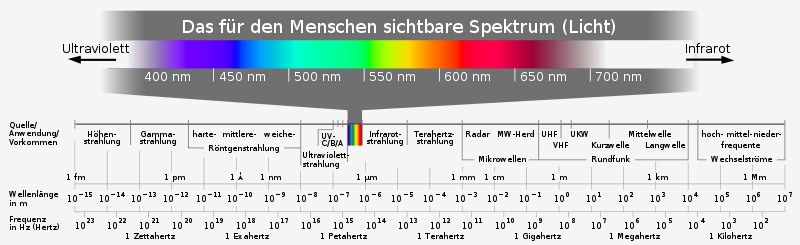
\includegraphics[width=\columnwidth]{pics/elektromagnetisches_Spektrum.png}
 \caption{Elektromagnetisches Spektrum mit dem für den Menschen sichtbaren Bereich des Spektrums.  \cite{elektromagnetisches_Spektrum}}
 \label{dsafigure:beispiel}
\end{dsafigure}

Das Sonnenlicht enthält alle Farben dieses Farbspektrums und erscheint deshalb weiß. Wenn die Lichtquelle ausgeschaltet ist, sehen wir schwarz, da kein Licht ausgestrahlt wird. Wird bei diesem additiven Farbsystem zum Beispiel das Licht von einer blauen und einer roten Lampe addiert, entsteht die Farbe Magenta (siehe Abbildung \ref{dsafigure:farbkreis}). Im Gegensatz dazu wird das Licht einer Lichtquelle (zum Beispiel der Sonne) von allen Gegenständen reflektiert. 
Bei diesem substraktivem Farbsystem ergibt sich die Farbe Schwarz aus der gemeinsamen Absorption von Wellenlängen aller Farben (siehe Abbildung \ref{dsafigure:farbkreis}).

Den Zusammenhang zwischen der Wellenlänge und der Energie lässt sich mit folgender Formel erklären:

\begin{equation}
E = \frac{h \cdot c}{\lambda} 
= h \cdot \nu
\end{equation}

$E$ beschreibt die Energie des Photons, $h$ das Plancksches Wirkungsquantum, $c$ die Lichtgeschwindigkeit, $\lambda$ die Wellenlänge, und $\nu$ die Frequenz.
Bei einer höheren Energie hat das Licht eine höhere Frequenz und dementsprechend ist die Wellenlänge kürzer. Umgekehrt bedeutet es auch, dass das Licht bei einer niedrigeren Energie eine niedrigere Frequenz und somit auch eine längere Wellenlänge hat.

\begin{dsafigure}
 \centering
 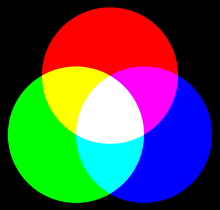
\includegraphics[width=0.45\columnwidth]{Additives_Farbsystem.png}
  \hfill
 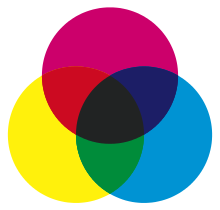
\includegraphics[width=0.45\columnwidth]{Substraktives_Farbsystem.png}
 \caption{Additives Farbsystem (links)\cite{Additives_Farbsystem} und Substraktives Farbsystem (rechts)\cite{Subtraktives_Farbsystem}}
 \label{dsafigure:farbkreis}
\end{dsafigure}


Der Zusammenhang zwischen Licht und Farbigkeit liegt an der Absorption und Reflexion von Licht. Dieses fällt durch die Pupille ins Auge und trifft dort auf die Netzhaut, die wiederum aus Stäbchen und Zapfen besteht. Die Stäbchen sind bei schwachen Lichteinfall aktiv und wir können damit nur schwarz-weiß sehen. Die Zapfen befinden sich im Zentrum der Netzhaut und sind besonders bei hohem Lichteinfall aktiv. Es gibt drei unterschiedliche Arten von Zapfen, die s-Zapfen, die als blaue Rezeptoren fungieren, die m-Zapfen, die als grüne Rezeptoren fungieren und die l-Zapfen, die als rote Rezeptoren fungieren. Jeder der Zapfen hat sein Maximum bei einer anderen Wellenlänge und zusammen decken sie somit den sichtbaren Bereich des elektromagnetischen Spektrums ab. 
Bei Anregung der Zapfen durch Licht, leiten sie einen Reiz an das Gehirn weiter. Durch die Kombination der verschiedenen angeregten Zapfen sehen wir Farbe.
Betrachten wir einen blauen Stift, der von der Sonne angeleuchtet wird, dann erscheint er uns blau. Was wir allerdings nicht sehen ist, dass die Elektronen im Stift vom Licht angeregt werden und vom Grundzustand in ein höheres Energieniveau angehoben werden (siehe Abbildung \ref{dsafigure:Grundzustand} ). Da dieser Zustand sehr instabil ist, fällt das Elektron wieder in seinen Grundzustand zurück. Dabei erfolgt die so genannten Relaxation über Schwingungen des Systems und es entsteht Wärme (siehe Abbildung \ref{dsafigure:Grundzustand}). Dass wir den Stift als blau wahrnehmen liegt daran, dass er die Komplementärfarbe zu Blau, also Gelb, absorbiert. Durch das fehlen der gelben Wellenlänge im reflektiertem Licht des Stiftes, interpretiert das Gehirn ihn als blau (siehe Abbildung \ref{dsafigure:farbkreis}, additives Farbsystem).
Wird blaues Licht durch einen Prozess emittiert, wird dieses ebenfalls als blau wahrgenommen.


\begin{dsafigure}
 \centering
 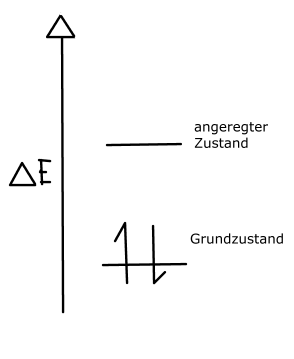
\includegraphics[width=0.45\columnwidth]{Grundzustand.png}
   \hfill
   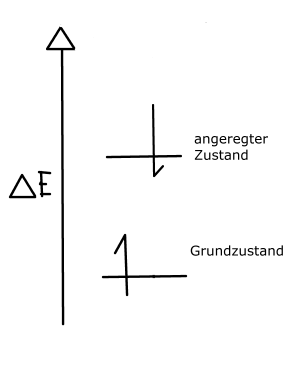
\includegraphics[width=0.45\columnwidth]{angeregter_Zustand.png}
 \caption{Elektronen im Grundzustand (links) und im angeregten Zustand (rechts)}
 \label{dsafigure:Grundzustand}
\end{dsafigure}


\section{Atomorbitale}
\authors{Johannes Wörsdörfer, Ali Serour}

Atomorbitale sind Einteilchen-Wellenfunktionen. Sie sind Lösungen der Schrödingergleichung für das Wasserstoffatom beziehungsweise für Ionen mit nur einem Elektron. Die Aufenthaltswahrscheinlichkeitsdichte der Elektronen ergibt sich aus dem Betragsquadrat der Funktion. Demnach erwies sich die Vorstellung, dass sich die Elektronen eines Atoms in Schalen bewegen, als unvollständig. Darauf wird im Kapitel Schrödingergleichung  näher eingegangen.

Atomorbitale werden mithilfe von vier Quantenzahlen klassifiziert. Die Hauptquantenzahl $n$ definiert das Energieniveau des Elektrons. Die Nebenquantenzahl $l$ bestimmt die Geometrie der Orbitale. Sie kann die Werte $l = 0, 1, ..., n-1$ annehmen. Die magnetische Quantenzahl $m$ beschreibt den Drehimpuls eines Elektrons und somit die Ausrichtung des Orbitals im Raum. Es gibt die magnetischen Quantenzahlen $m = -l,...,l$. Die vierte Zahl ist die Spinquantenzahl $s$. Diese kann die Werte $s = -\frac{1}{2}, \frac{1}{2}$ annehmen \cite{Riedel07}. 

Um größere Atome beschreiben zu können, bedienen wir uns einer Näherung: Wir konstruieren die Vielteilchenwellenfunktion mithilfe von Einteilchenwellenfunktionen, die mit Elektronen besetzt werden. Dabei müssen drei Regeln beachtet werden: Das Aufbauprinzip besagt, dass zuerst alle energieärmeren Niveaus besetzt werden, bevor das darüber liegende Orbital besetzt wird. Die Hundsche Regel schreibt vor, dass bei einer Entartung eines Orbitals zuerst alle Orbitale mit gleicher Nebenquantenzahl $l$ mit dem gleichen Spin besetzt werden. Das Pauli-Prinzip gibt an, dass ein Orbital nur mit zwei Elektronen mit entgegengesetztem Spin besetzt werden kann, da es nicht zwei Elektronen mit exakt den selben Quantenzahlen innerhalb eines Atoms geben darf.

Im Folgenden wird dieses Modell anhand des Kohlenstoffatoms mithilfe eines Energieniveaudiagramms illustriert (siehe Abb. \ref{fig:Energieniveaudiagramm}). Kohlenstoff hat die Ordnungszahl 6. Es besitzt somit 6 Elektronen. Die Orbitale werden von unten nach oben mit Elektronen aufgefüllt, da Elektronen die energetisch günstigste Anordnung anstreben.  Die Elektronenkonfiguration für Kohlenstoff lautet $1s^{2} 2s^{2} 2p^{2}$. Die vorderen Zahlen geben die Hauptquantenzahl an. Der Buchstabe bezeichnet die Nebenquantenzahl der Orbitale mit $s$ für $l = 0$ und $p$ für $l=1$ und der Exponent definiert die Anzahl der Elektronen im jeweiligen Orbital.

\begin{dsafigure}
 \centering
 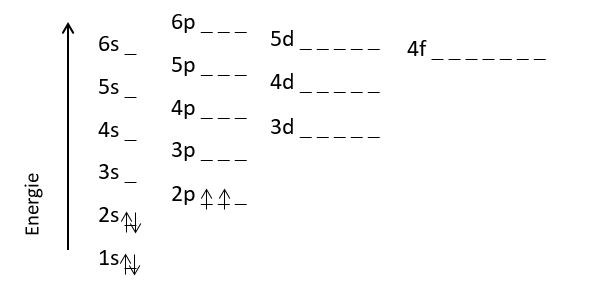
\includegraphics[width=8cm]{Energieniveaudiagramm.png}
 \caption{Die Besetzung der Orbitale nach dem Aufbauprinzip, der Hunschen Regel und dem Pauli-Prinzip ist anhand des Kohlenstoffatoms mithilfe eines Energieniveaudiagramms illustriert.}
 \label{fig:Energieniveaudiagramm}
\end{dsafigure}

Zum besseren Verständnis betrachten wir nun die räumliche Gestalt der Orbitale. Das s-Orbital hat die Form einer Kugel (siehe Abb. \ref{fig:s}). Die Nebenquantenzahl beträgt $0$. Außerdem hat es keine Knotenebene. Das p-Orbital hat die Nebenquantenzahl 1. Es gibt genau drei Magnetquantenzahlen $m = -1, 0, 1$. Das Orbital mit der magnetischen Quantenzahl $0$ hat die Form einer Hantel entlang der $z$-Achse. Es wir auch als $p_{z}$ bezeichnet (siehe Abb. \ref{fig:pz}). Aus den Zuständen $m = -1$ und $1$ werden die Linearkombinationen $p_{x} = \frac{1}{\sqrt{2}} (p_{+1} - p_{-1})$ (siehe Abb. \ref{fig:px}) und $p_{y} = \frac{i}{\sqrt{2}}(p_{+1}+p_{-1})$ (siehe Abb. \ref{fig:py} ) gebildet. Gleiches lässt sich auch auf d-Orbitale übertragen (siehe Abb. \ref{fig:dz2} - \ref{fig:dyz}).

\begin{dsafigure}
 \centering
 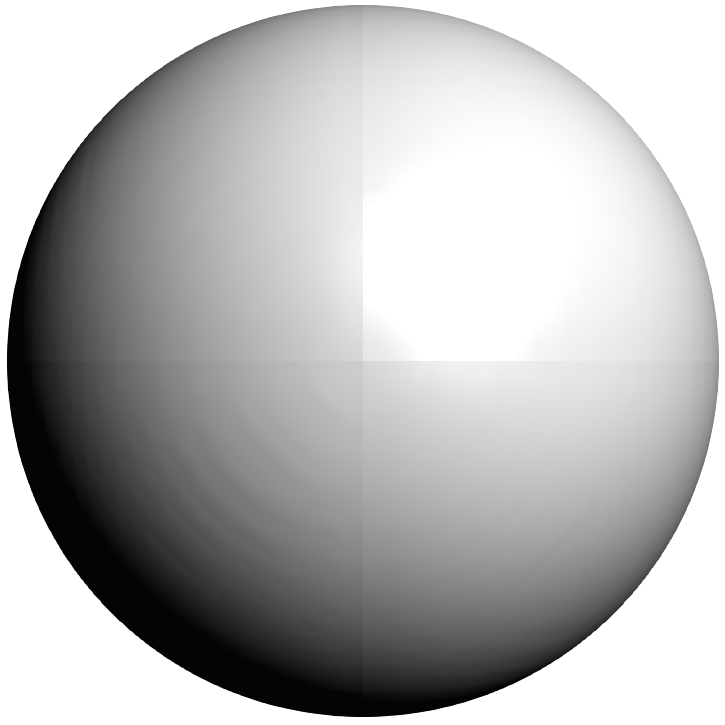
\includegraphics[width=8cm]{s.png}
 \caption{Darstellung eines s-Orbitals \cite{ADF2017authors}.}
 \label{fig:s}
\end{dsafigure}

\begin{dsafigure}
 \centering
 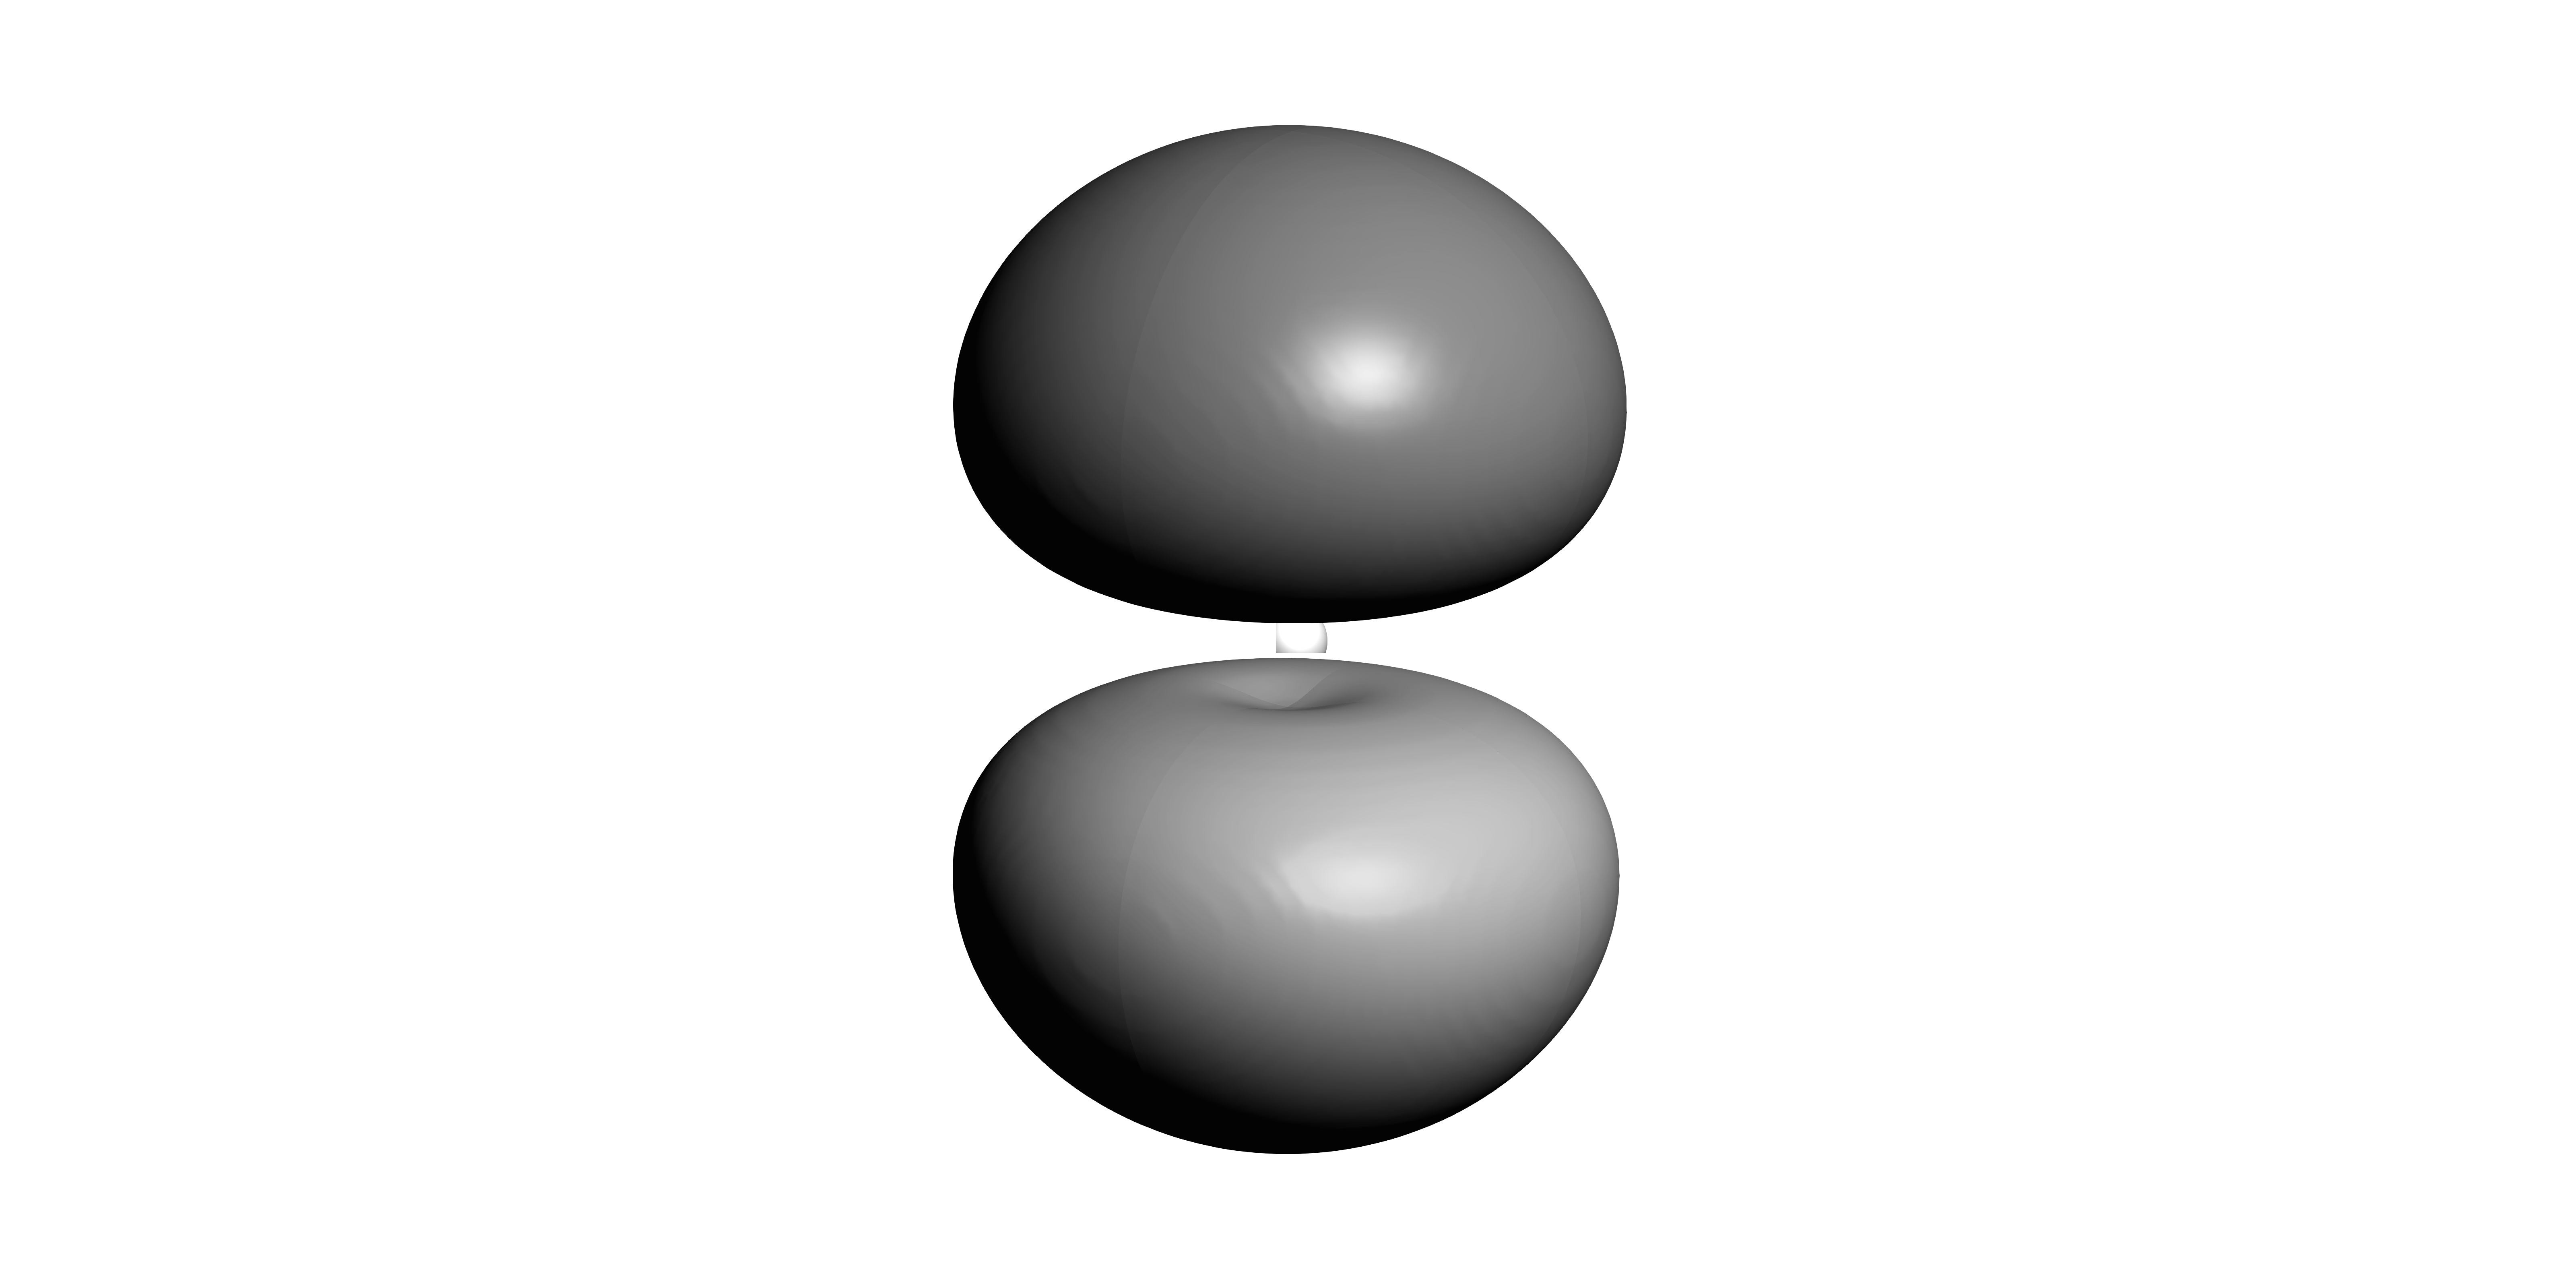
\includegraphics[width=8cm]{pz.png}
 \caption{Darstellung eines p$_{z}$-Orbitals \cite{ADF2017authors}.}
 \label{fig:pz}
\end{dsafigure}

\begin{dsafigure}
 \centering
 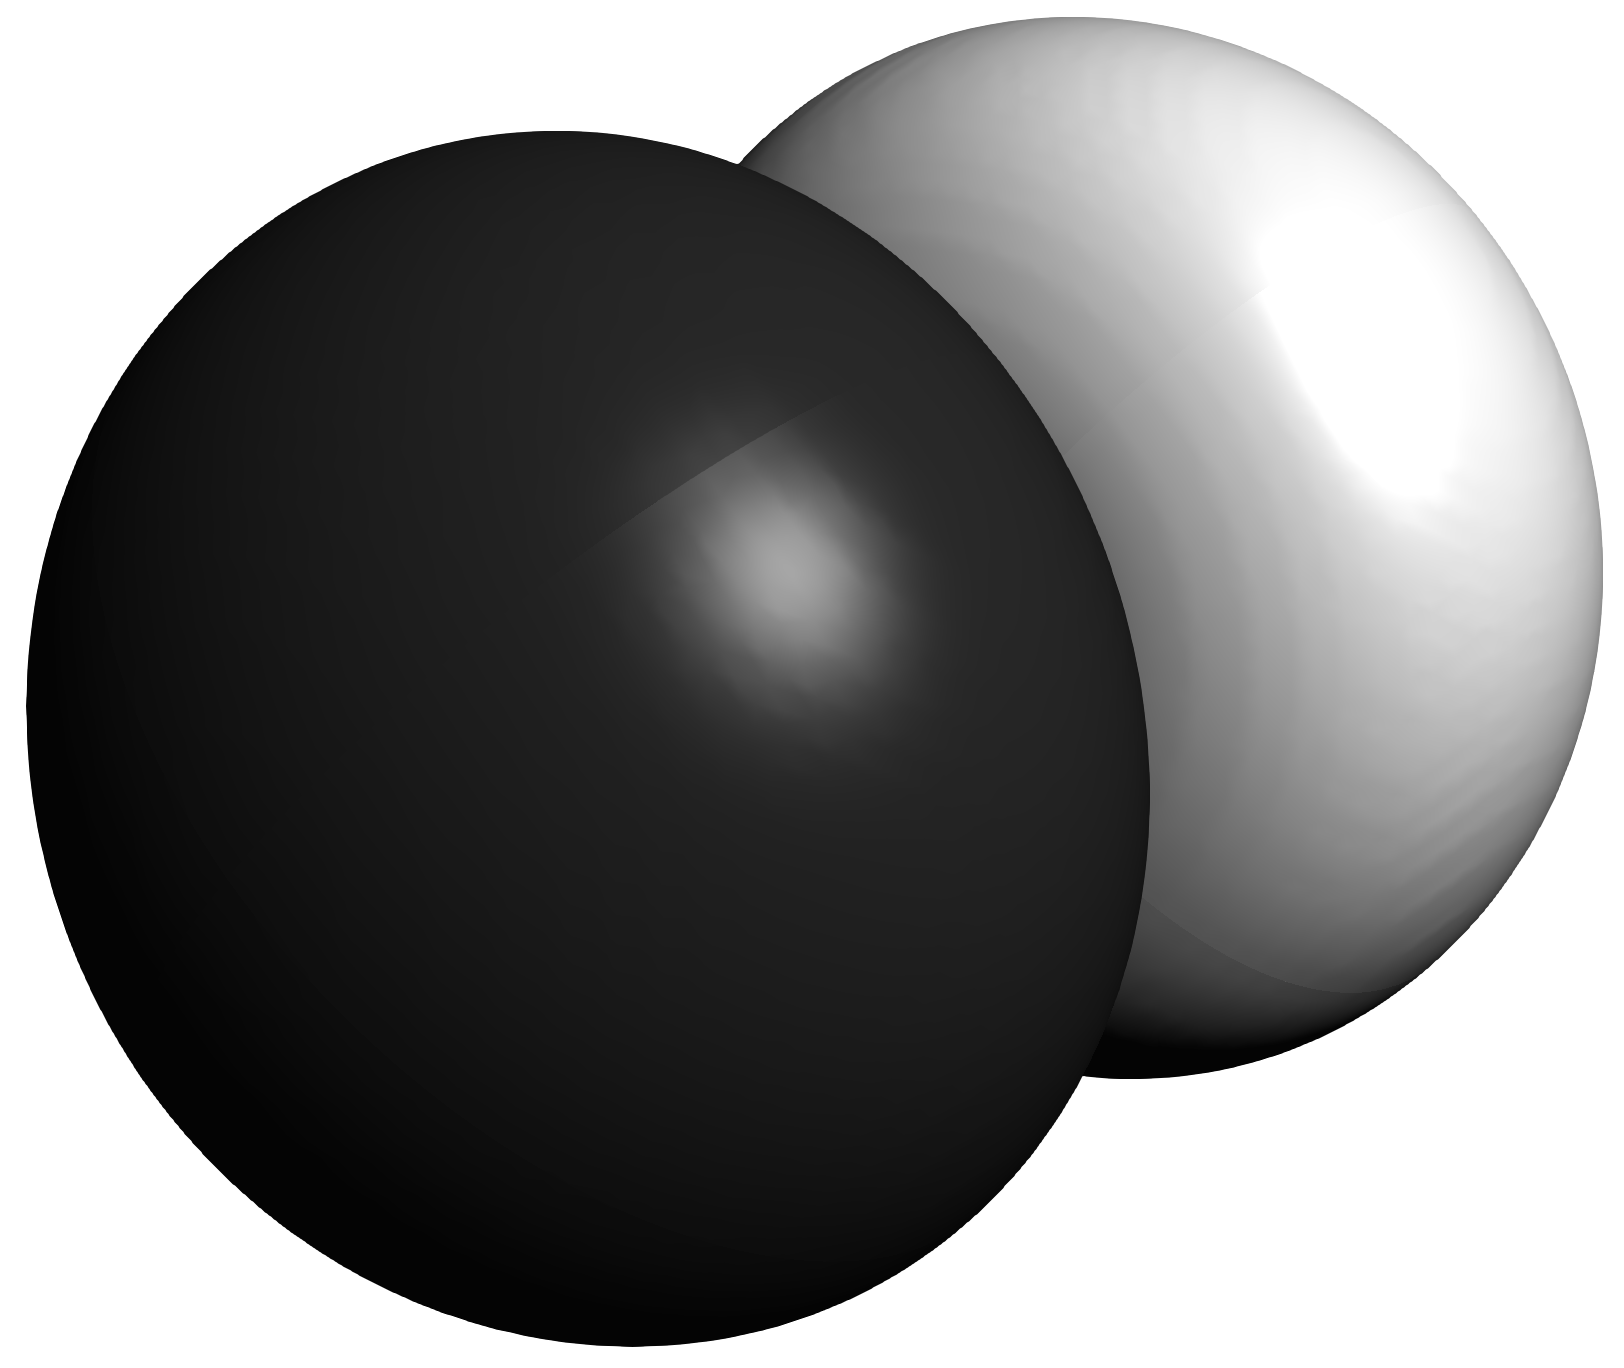
\includegraphics[width=8cm]{px.png}
 \caption{Darstellung eines p$_{x}$-Orbitals \cite{ADF2017authors}.}
 \label{fig:px}
\end{dsafigure}

\begin{dsafigure}
 \centering
 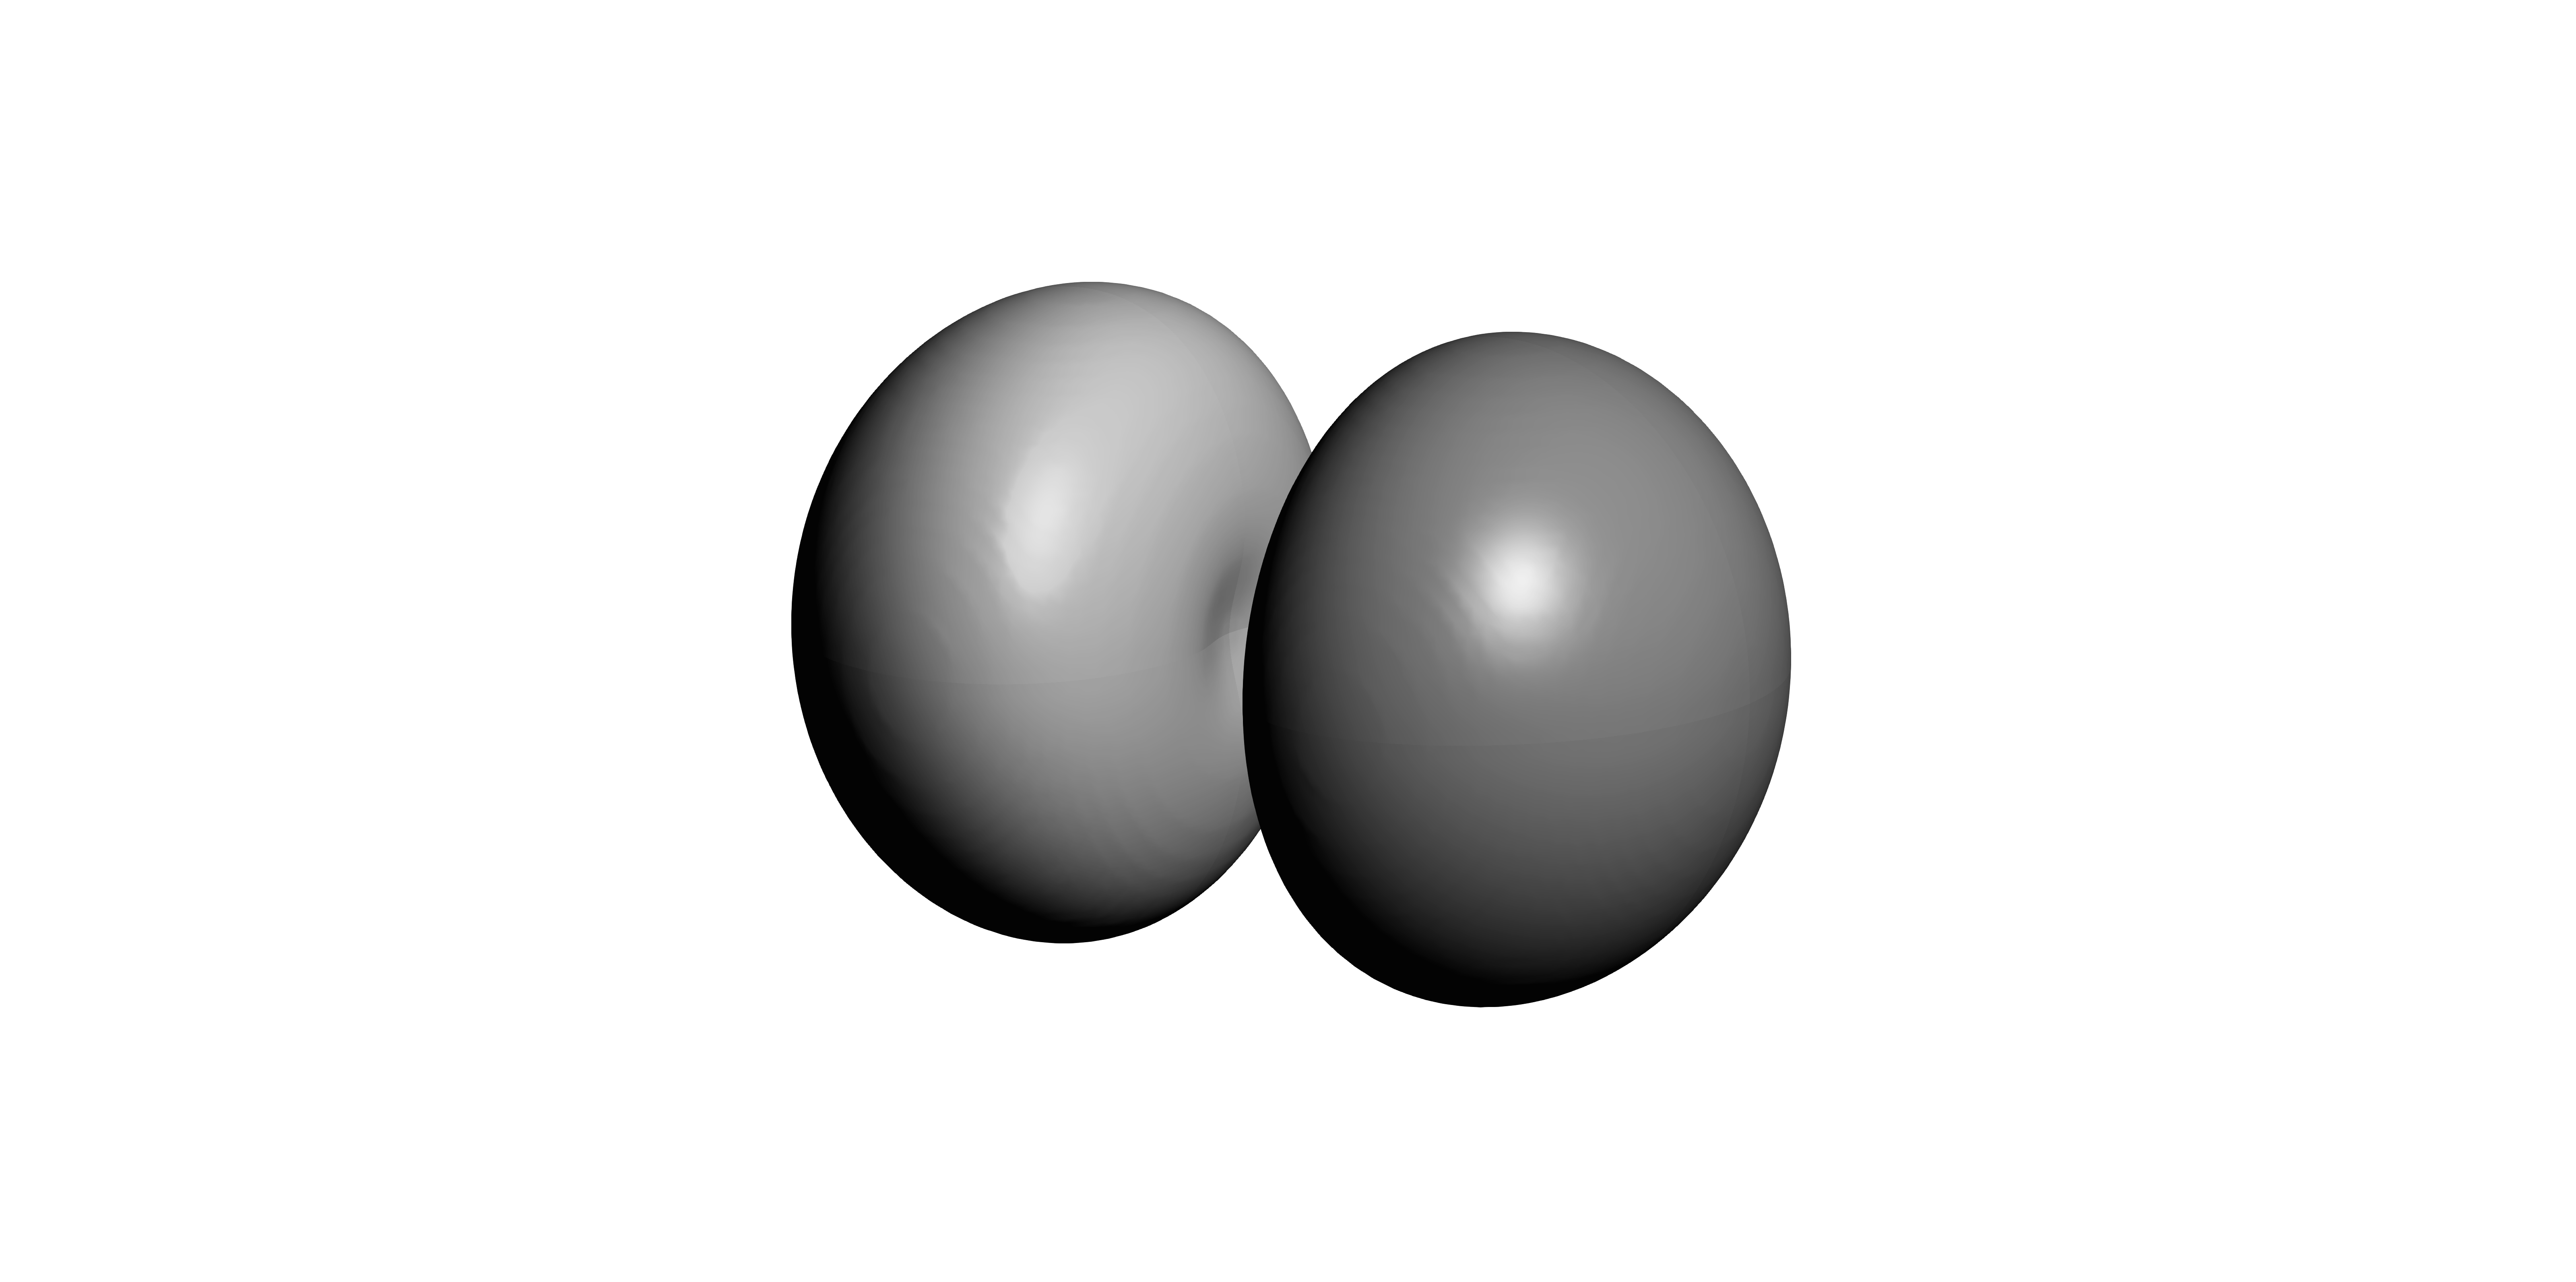
\includegraphics[width=8cm]{py.png}
 \caption{Darstellung eines p$_{y}$-Orbitals \cite{ADF2017authors}.}
 \label{fig:py}
\end{dsafigure}

\begin{dsafigure}
 \centering
 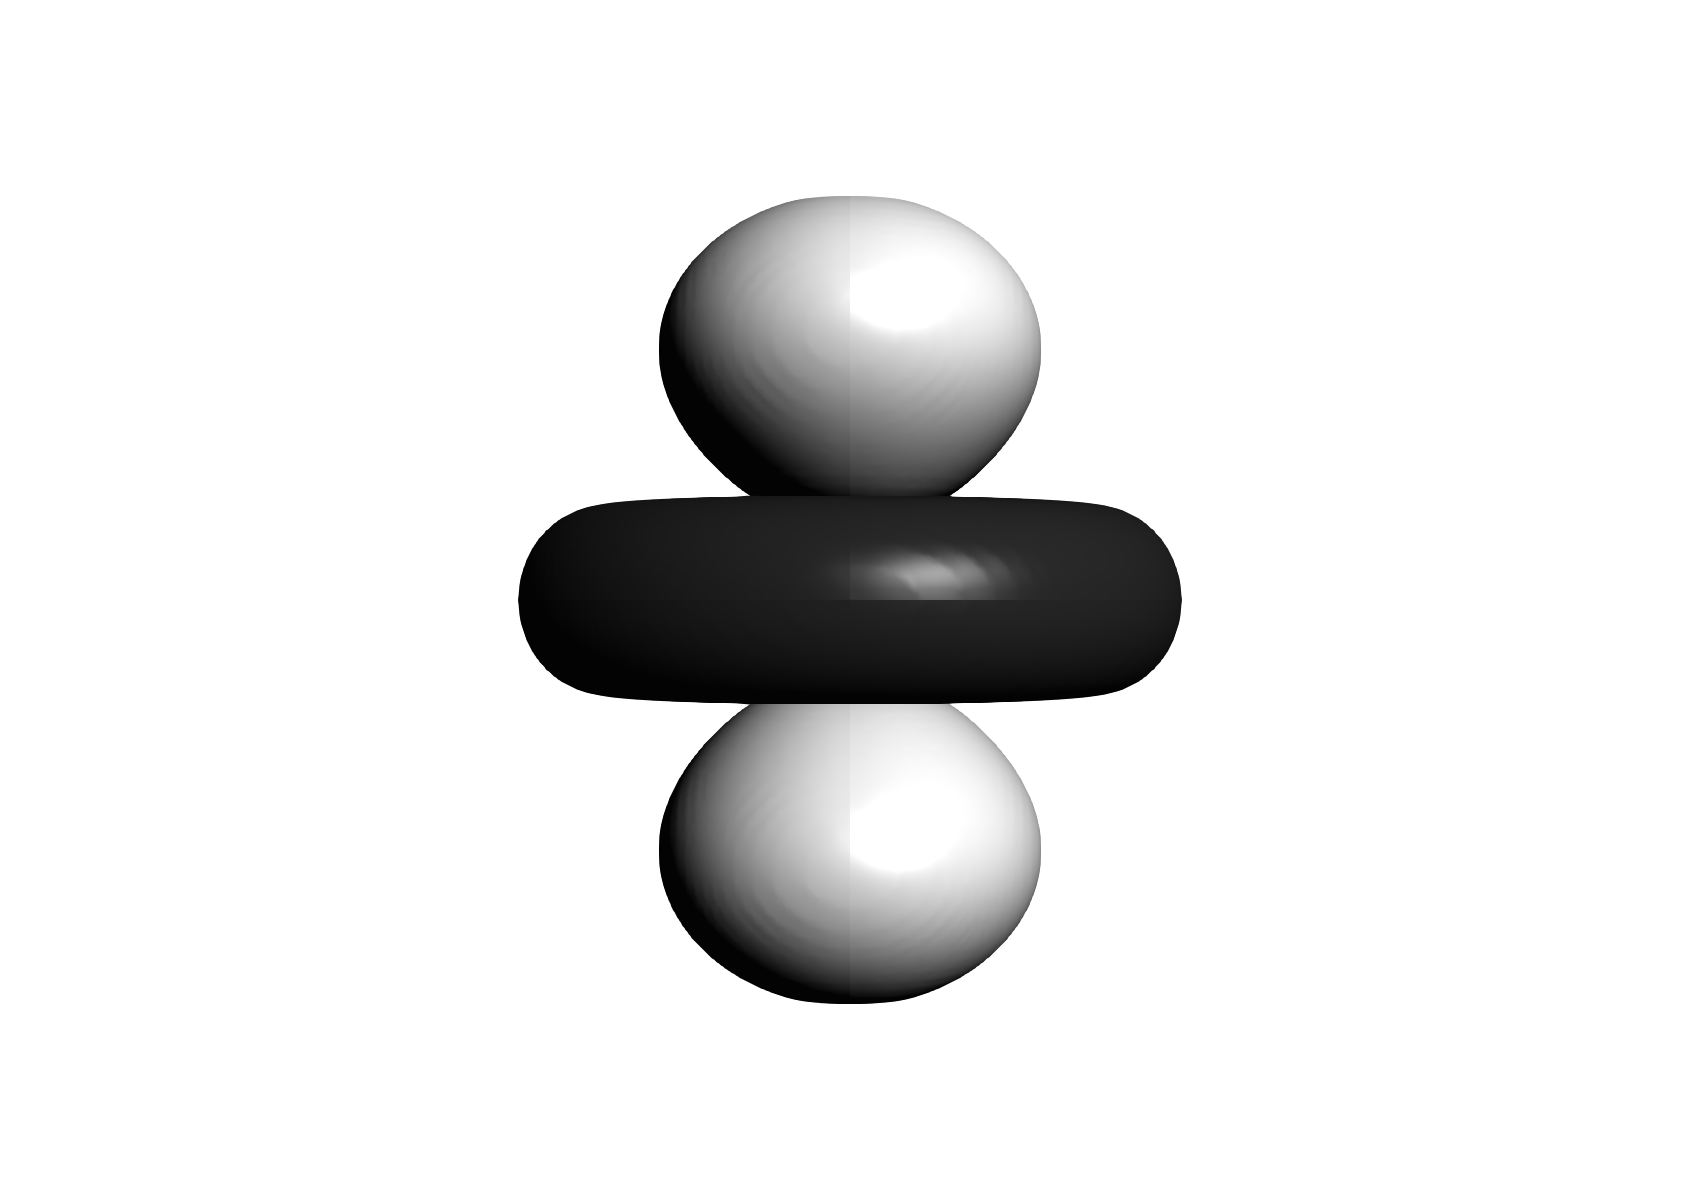
\includegraphics[width=8cm]{dz2.png}
 \caption{Darstellung eines d$_{z^{2}}$-Orbitals \cite{ADF2017authors}.}
 \label{fig:dz2}
\end{dsafigure}

\begin{dsafigure}
 \centering
 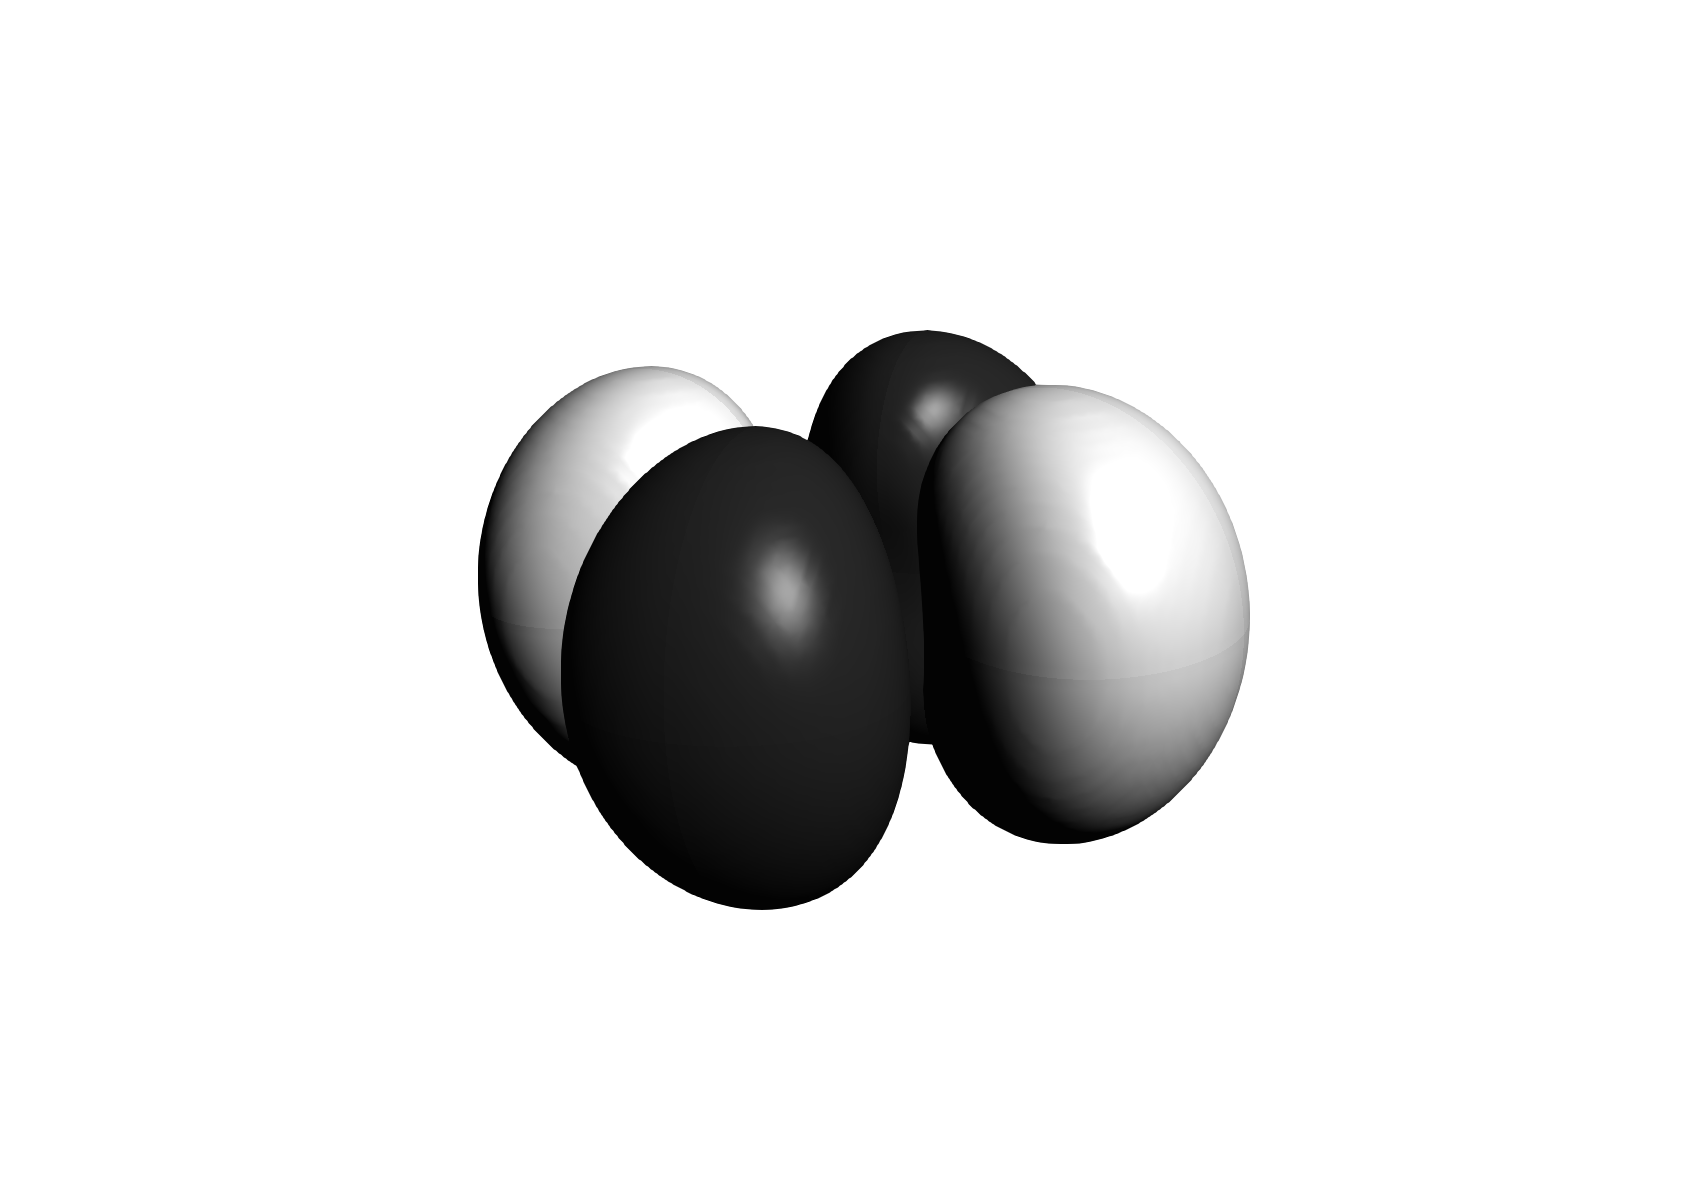
\includegraphics[width=8cm]{dx2-y2.png}
 \caption{Darstellung eines d$_{x^{2}-y^{2}}$-Orbitals \cite{ADF2017authors}.}
 \label{fig:dx2-y2}
\end{dsafigure}

\begin{dsafigure}
 \centering
 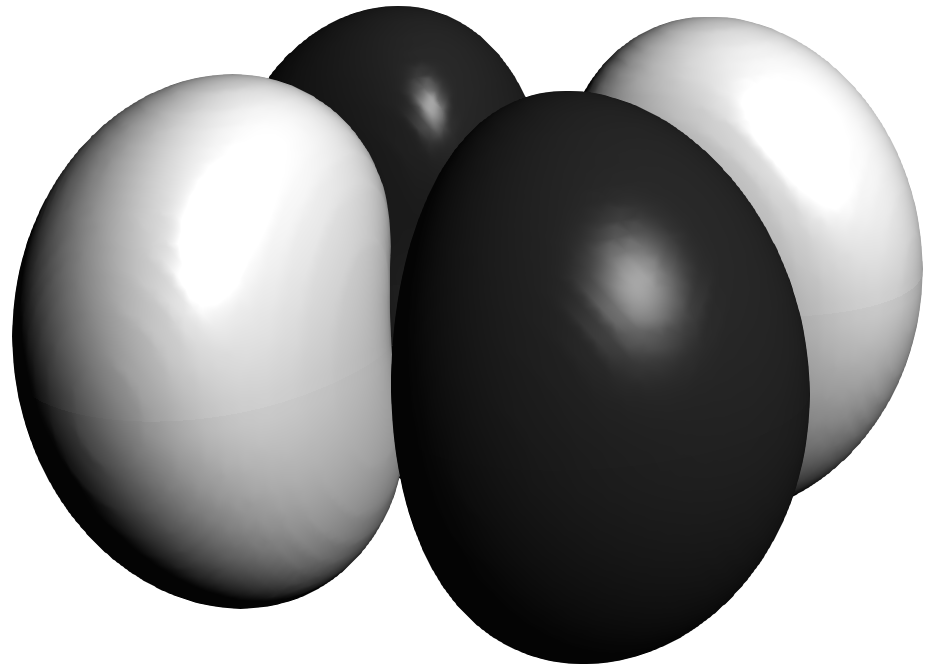
\includegraphics[width=8cm]{dxy.png}
 \caption{Darstellung eines d$_{xy}$-Orbitals \cite{ADF2017authors}.}
 \label{fig:dxy}
\end{dsafigure}

\begin{dsafigure}
 \centering
 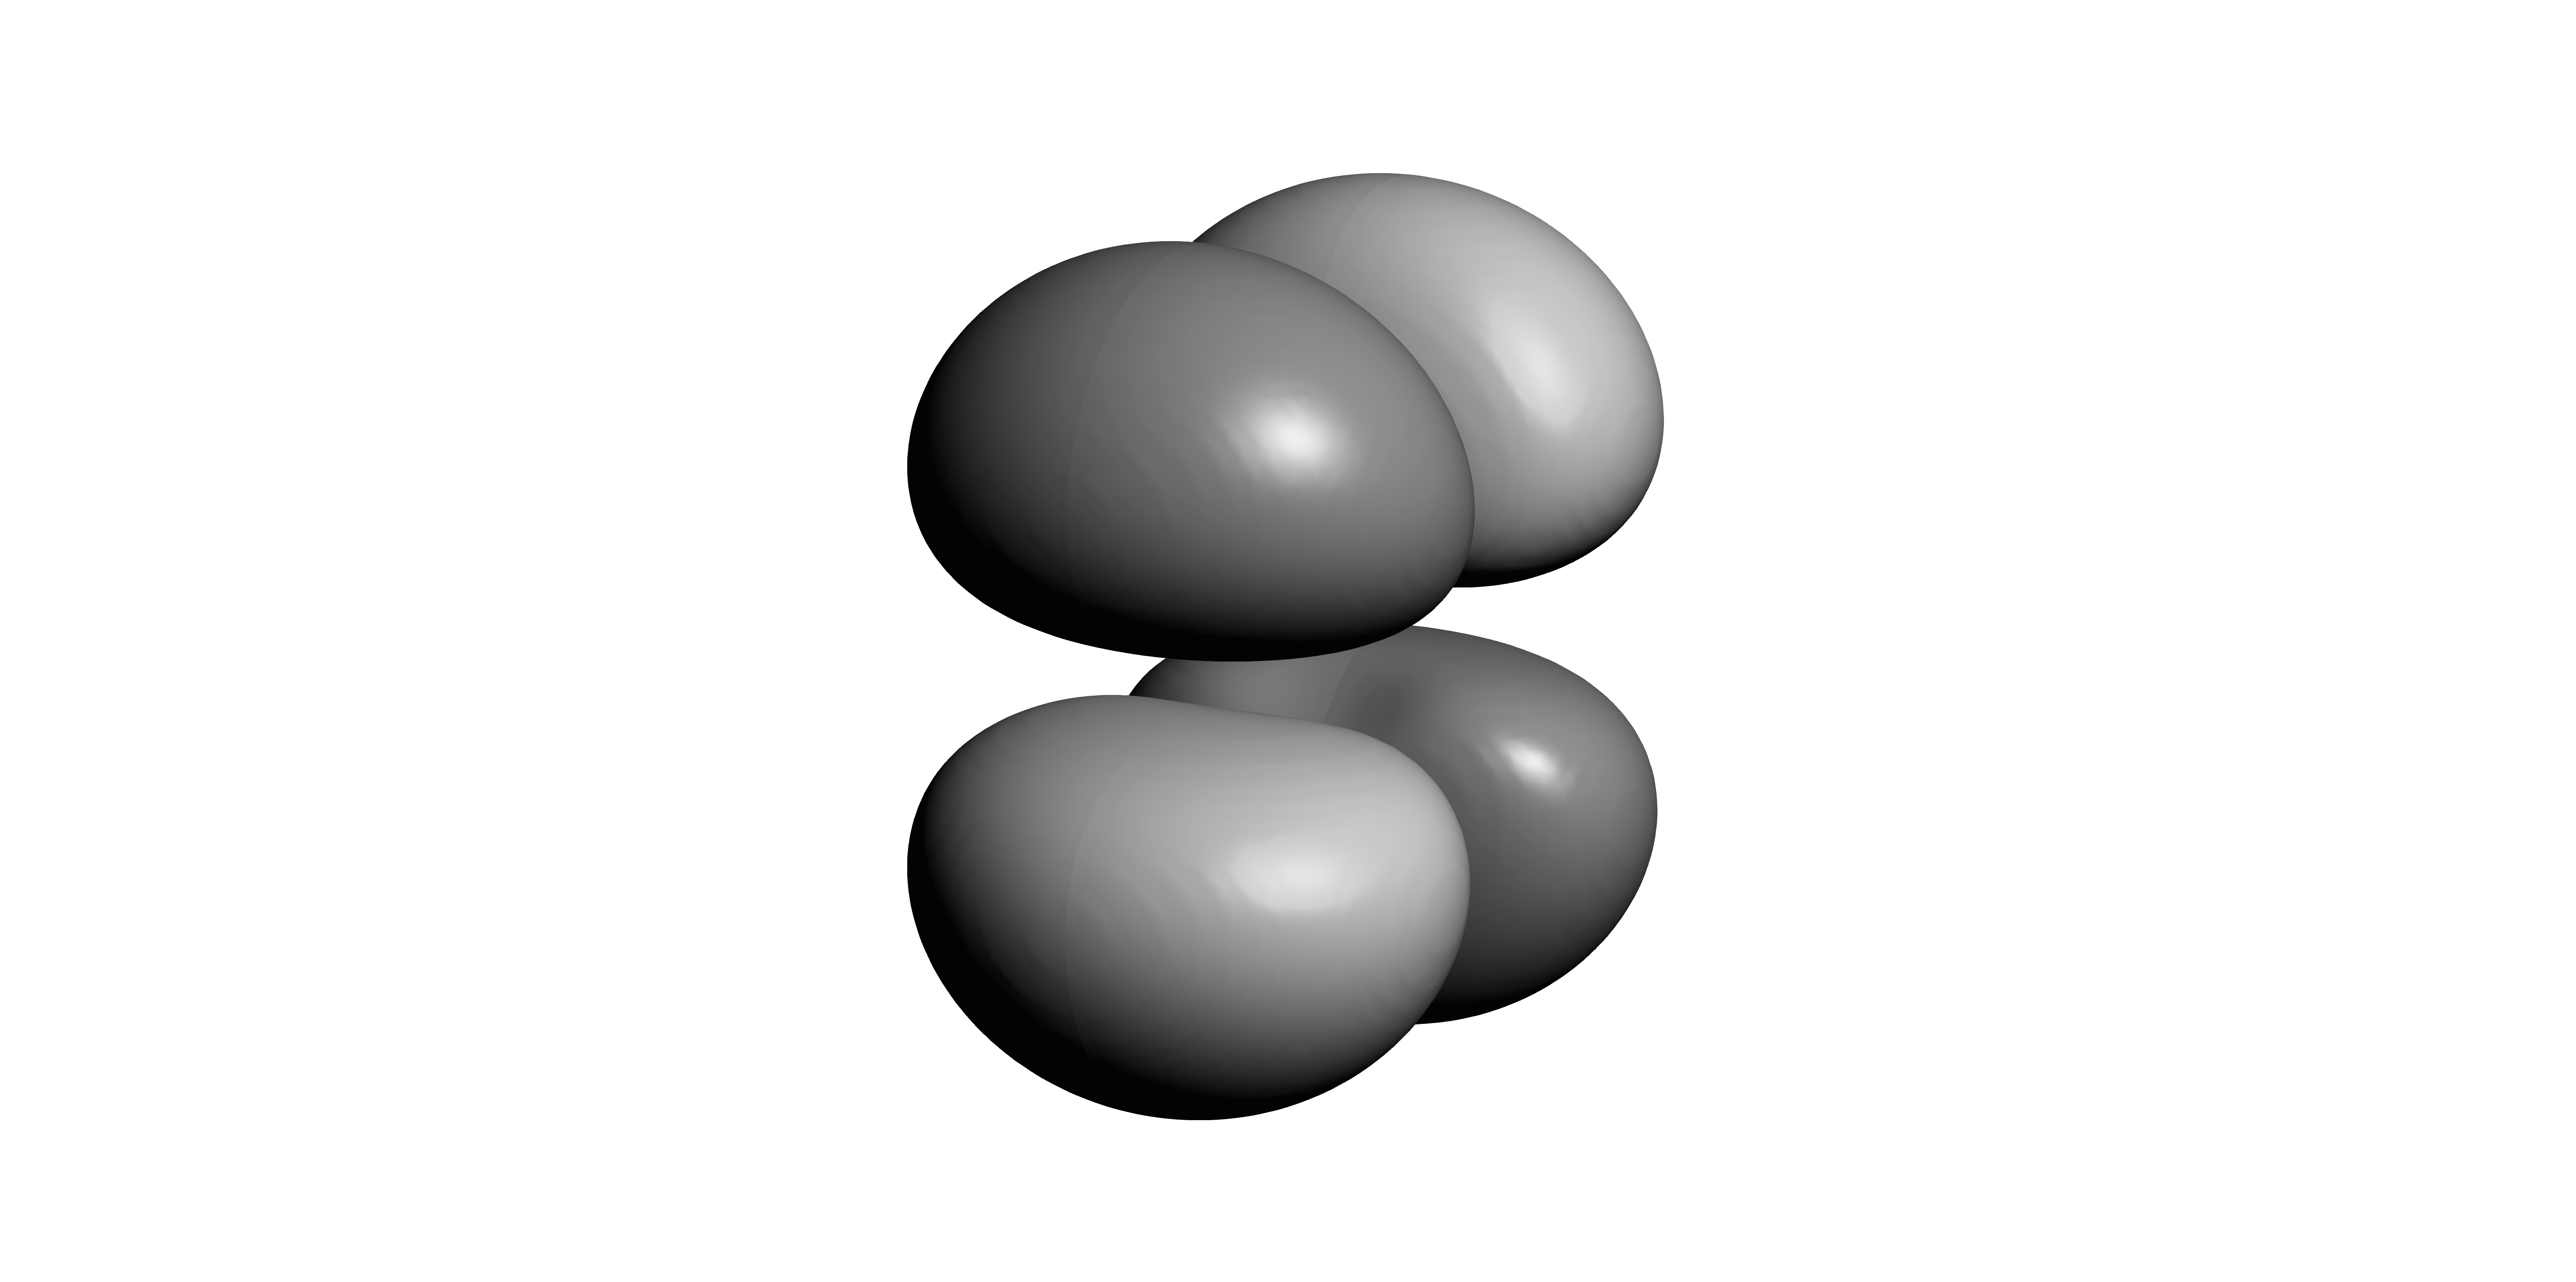
\includegraphics[width=8cm]{dxz.png}
 \caption{Darstellung eines d$_{xz}$-Orbitals \cite{ADF2017authors}.}
 \label{fig:dxz}
\end{dsafigure}

\begin{dsafigure}
 \centering
 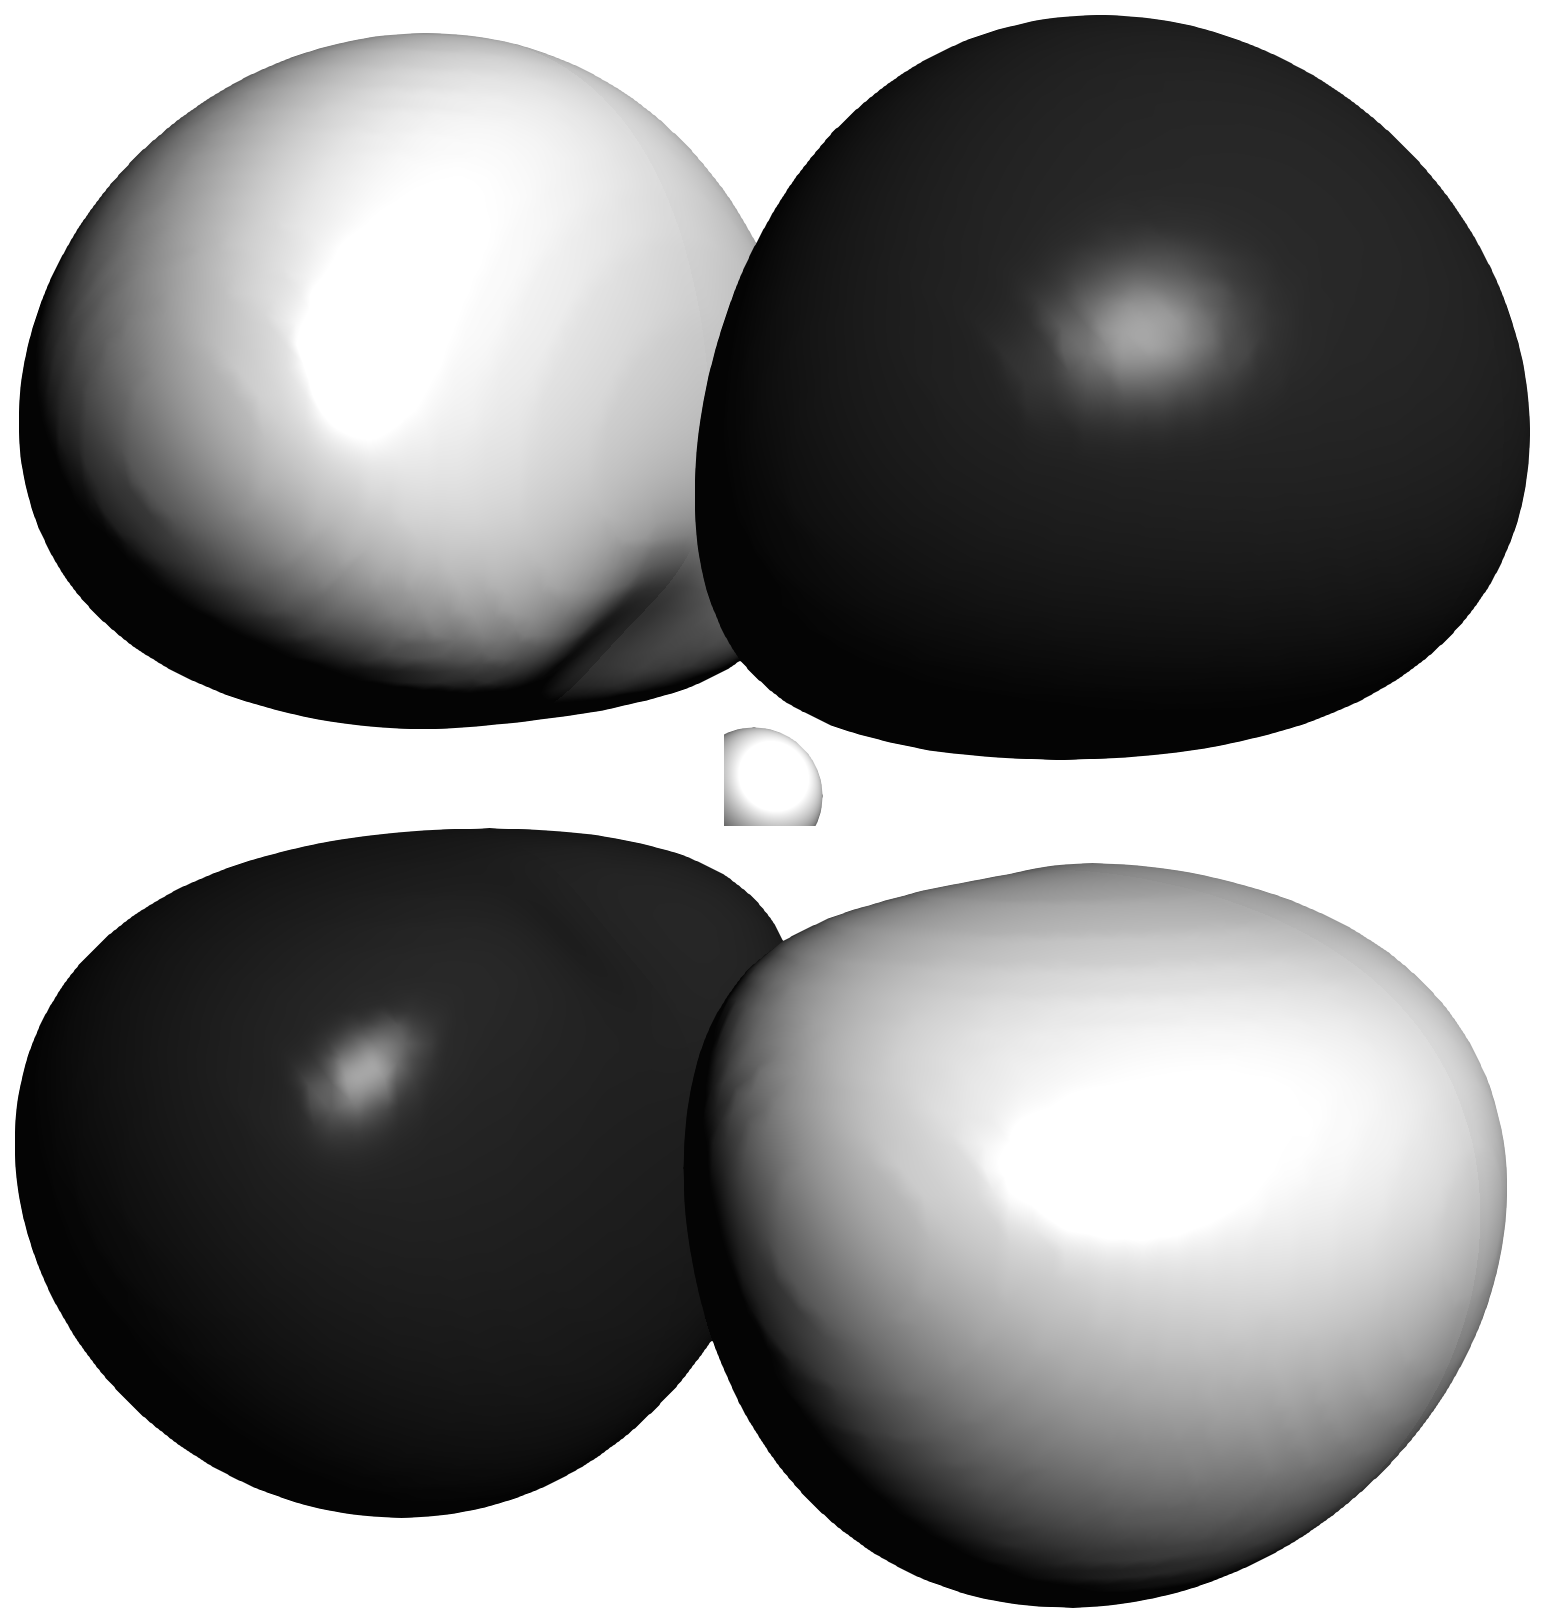
\includegraphics[width=8cm]{dyz.png}
 \caption{Darstellung eines d$_{yz}$-Orbitals \cite{ADF2017authors}.}
 \label{fig:dyz}
\end{dsafigure}


\section{Welle-Teilchen-Dualismus}

Autoren: Patricia Mühren, Kristina Heuser

Das Doppelspaltexperiment mit Photonen und Elektronen sowie der photoelektrische Effekt zeigen auf, dass Licht und Elektronen sowohl Wellen- als auch Teilchencharakter haben.

Zunächst kann das Doppelspaltexperiment mit Kugeln veranschaulicht und theoretisch betrachtet werden. Dabei werden Kugeln von einer Quelle ausgesendet und passieren zwei schmale, parallele Spalten. Auf einem Beobachtungsschirm in einiger Entfernung kann man daraufhin erkennen, dass die Verteilung beziehungsweise die Ankunftswahrscheinlichkeit für klassische Teilchen der Summe der beiden Einzelspaltverteilungen entspricht (vergleiche Abbildung \ref{dsafigure:beispiel1}). Im nächsten Schritt wird das Gedanken-Doppelspaltexperiment mit Wellen ausgeführt. Hier weist die Verteilung ein Interferenzmuster auf. Dies lässt sich dadurch erklären, dass die Maxima der Verteilungsfunktion genau an den Orten konstruktiver Überlagerung liegen (vergleiche Abbildung \ref{dsafigure:beispiel2}). 

\begin{dsafigure}
\centering
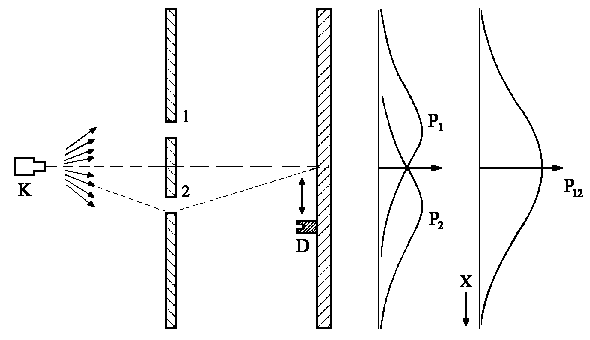
\includegraphics[scale=0.5]{Kugeln.png}
\caption{Das Doppelspaltexperiment mit Kugeln. \cite{Doppelspalt}}
\label{dsafigure:beispiel1}
\end{dsafigure}

\begin{dsafigure}
\centering
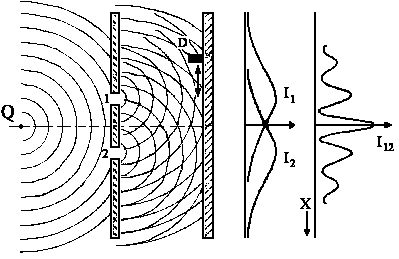
\includegraphics[scale=0.5]{Wellen.png}
\caption{Das Doppelspaltexperiment mit Wellen. \cite{Doppelspalt}}
\label{dsafigure:beispiel2}
\end{dsafigure}

Die Durchführung des Experimentes mit Elektronen zeigt, dass die Verteilungsfunktion der Elektronen nicht der Summe der beiden Einzelspaltverteilungen entspricht, wie sich Abbildung \ref{dsafigure:beispiel3} entnehmen lässt. Daher weisen Elektronen Welleneigenschaften auf. Ebenso zeigt Licht im Doppelspaltexperiment Interferenzen und, einhergehend damit, auch die Eigenschaften einer Welle. 

\begin{dsafigure}
\centering
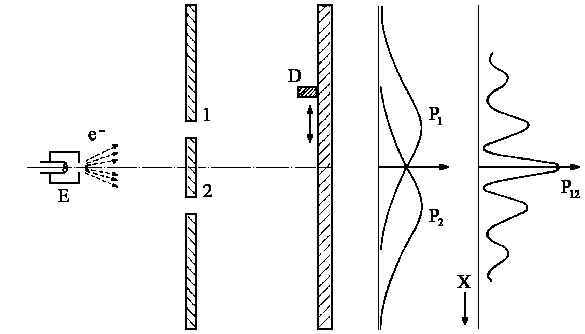
\includegraphics[scale=0.5]{Elektronen.png}
\caption{Das Doppelspaltexperiment mit Elektronen. \cite{Doppelspalt}}
\label{dsafigure:beispiel3}
\end{dsafigure}

Paradoxer Weise illustriert der photoelektrische Effekt, bei dem durch Auftreffen von Licht auf eine Metalloberfläche Elektronen emittiert werden, dass Licht ebenso Teilchencharakter aufweist, der der Wellennatur zuwider zu laufen scheint. Die Beobachtung gleichbleibender Energie der emittierten Elektronen bei zunehmender Intensität des Lichtes widerspricht der aus der klassischen Wellenbeschreibung abgeleiteten Folgerung, dass eine Zunahme der Intensität zu einem Anstieg der kinetischen Energie des herausgelösten Elektrons führen müsste. Dieser Umstand kann mit Teilchencharakter von Elektronen erklärt werden. Analog dazu wird derselbe Versuch mit Elektronen realisiert -- mit dem gleichen Ergebnis wie bei Licht.
Die Tatsache, dass Licht und Elektronen sowohl Wellen-, als auch Teilchencharakter besitzen, wird mit dem Welle-Teilchen-Dualismus addressiert. Sie ist aus einer rein klassischen Anschauung heraus nicht zu erklären und fordert eine neue Theorie \cite{Feynman_lectures70}.



\section{Die Schrödingergleichung}
\authors{Lena Trahe, Lynn Meeder}

Um die Struktur, Energie und Eigenschaften von Atomen und Molekülen zu beschreiben, bedient man sich der Quantenmechanik \cite{Reinhold}.

\subsection{Operatoren und Eigenwertprobleme}

Wendet man einen Operator $\hat{A}$ auf eine Funktion $f(x)$ an, so erhält man eine neue Funktion $g(x)$. Ein bekannter Operator ist zum Beispiel der Differentialoperator  $\frac{d}{dx}$.

Für einen solchen Operator lässt sich eine Eigenwertproblem formulieren, in dem $g(x)= af(x)$ und somit folgende Gleichung gilt:

\begin{equation}
\hat{A}f(x)=af(x)
 \label{OperatorEigenwert}
\end{equation}

Gesucht sind nun die Eigenfunktionen $f(x)$ und die Eigenwerte a, die Gleichung \ref{OperatorEigenwert} genügen.

\subsection{Zeitunabhängige Schrödingergleichung}

Die zeitunabhängige Schrödingergleichung ist das Eigenwertproblem des Hamilton-Operators $\hat{H}$:

\begin{equation}
\hat{H} \psi = E \psi
\end{equation}

Der Hamilton-Operator ist der Operator der Gesamtenergie $E$. Die Gesamtenergie ist die Summe aus kinetischer Energie $T$, die vom Impuls $\vec{p}$ abhängt, und potentieller Energie $V$, die vom Ort $\vec{x}$ abhängt. Analog ist der Hamilton-Operator die Summe aus den Operatoren für die kinetische und die potentielle Energie:

\begin{equation}
\hat{H}(\hat{\vec{p}}, \hat{\vec{x}}) = \hat{T} (\hat{\vec{p}}) + \hat{V} (\hat{\vec{x}})
\label{HamiltonOperatorTV}
\end{equation}

$\hat{\vec{p}}$ ist somit der Impulsoperator und $\hat{\vec{x}}$ der Ortsoperator. Die kinetische Energie $T$ wird in der klassischen Mechanik als $\frac{\vec{p}^2}{2m}$ beschrieben. Den Impulsoperator $\hat{\vec{p}}$ stellt man in der Quantenmechanik nun dar als 

\begin{equation}
\hat{\vec{p}} = -i\hbar \left( 
\begin{array}{c}
\frac{\partial}{\partial x} \\ \frac{\partial}{\partial y} \\ \frac{\partial}{\partial z}
\end{array} \right)
\end{equation}

Durch Einsetzen in den Ausdruck $\hat{T}=\frac{\hat{\vec{p}}^2}{2m}$ erhält man:

\begin{equation}
\hat{T}=-\frac{\hbar^2}{2m}  \left( \frac{\partial ^2}{\partial  x^2}+\frac{\partial ^2}{\partial  y^2}+\frac{\partial ^2}{\partial  z^2}\right)
\end{equation}

Die potentielle Energie hängt nur vom Ort $\vec{x}$ ab und ist deshalb in der Ortsdarstellung ein multiplikativer Operator: $\hat{V}(\hat{x})=\hat{V}(x)$. Die potentielle Energie eines Elektrons mit der Ladung $-e$ im Feld eines Protons mit der Ladung $+e$ beträgt $\hat{V}(x) = -\frac{1}{4 \pi \epsilon_0}\frac{e^2}{r}$. r bezeichnet die Entfernung des Elektrons zum Kern. Für das Wasserstoffatom lautet Gleichung \ref{HamiltonOperatorTV} also:

\begin{equation}
\left[ - \frac{\hbar^2}{2m}  \hat{\vec{\nabla}}^2 -\frac{1}{4 \pi \epsilon_0}\frac{e^2}{r} \right] \psi = E\psi
\end{equation}

Wobei der Operator $\hat{\vec{\nabla}}^2$ gegeben ist als:

\begin{equation}
\hat{\vec{\nabla}}^2 = \frac{\partial ^2}{\partial  x^2}+\frac{\partial ^2}{\partial  y^2}+\frac{\partial ^2}{\partial  z^2}
\end{equation}

Die diskreten Energieeigenwerte $E$ sind hier:

\begin{equation}
E_n=-\frac{m_e e^4}{2\hbar^2}\frac{1}{n^2} \:mit \: n\in \mathbb{N}
\end{equation}

\section{Das Teilchen im Kasten}
\authors{Atousa Seyedian, Ole Simmering}

\subsection{Allgemein}

Das Modell des Teilchens im Kasten ist ein eindimensionales Modell, welches als Näherung einer chemischen Bindung aufgefasst werden kann. In dem Kasten wird die potentielle Energie für $ 0 \leq x \leq L $ mit null gleich gesetzt.
Hier gilt also $ V_x = 0 $. 
Der Kasten ist begrenzt von Wänden an den $ x $-Werten $ x = 0 $ und $ x=L $. Außerhalb des Kastens ist das Potential unendlich (siehe Abbildung \ref{Potential im Kasten}).


\begin{dsafigure}
 \centering
 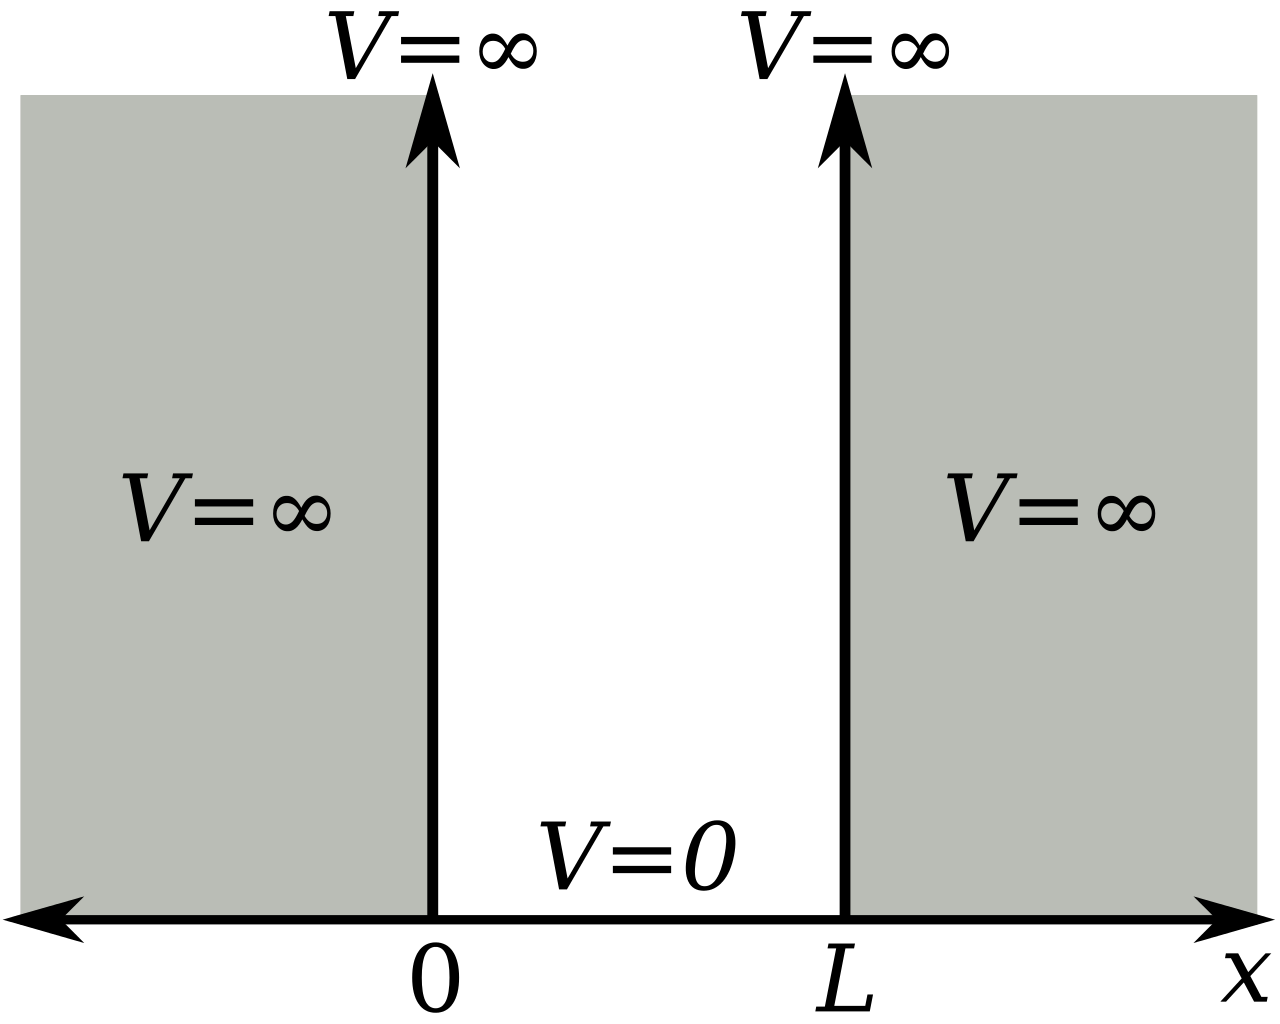
\includegraphics[width=8cm]{potential_kasten.png}
 \caption{Darstellung des Potentials im Modell des Teilchens im Kasten.
\cite{wikiKastenpot}}
 \label{Potential im Kasten}
\end{dsafigure} 

Die allgemeine Form der Schrödinger Gleichung lautet $ E\psi=\hat{H}\psi $. Der Hamilton-Operator $ \hat{H} $ ist der Operator für die kinetische und potentielle Energie eines Teilchens $ \hat{H}=\hat{T}+\hat{V} $. Da im Modell die potentielle Energie innerhalb des Kastens verschwindet, lässt sich der Hamilton Operator mit dem Operator der kinetischen Energie gleich setzen: $ \hat{H}=\hat{T} $. Damit lautet die Schrödingergleichung \cite{Atkins2001}:
\begin{equation}
E \psi = - \dfrac{\hbar ^2}{2m} \dfrac{d^2}{dx^2}\psi  
\end{equation}
 

Ein möglicher Ansatz für die Wellenfunktion ist $ \psi (x) = A \cdot \sin (kx) + B \cdot \cos (kx) $. Da die Wellenfunktion stetig sein muss und die Randbedingungen besagen, dass die Wellenfunktion bei $ x=0 $ und $ x=L$  den Wert $0$ annehmen muss, muss der Parameter $ B $ gleich $0$ gesetzt werden, sodass die Formel nach Einsetzen der Randbedingungen auf $ \psi (x) = A \cdot \sin (kL) $ reduziert werden kann. Dabei muss $ kL $ aufgrund der Randbedingungen ein ganzzahliges Vielfaches von $ n\cdot\pi $ sein. Die Wellenlänge $\lambda $ muss abhängig von der Länge $ L $ des Kastens sein. Es gilt: $ \lambda = n\pi/L $ mit $ n \in \mathbb{N} $. Somit muss $ k=n\pi/L $ sein. Die Wellenfunktion ist nun:
 
\begin{equation}
\psi (x) = A \sin \left(\dfrac{n \pi}{L} x\right)
\end{equation}
    
und nach Normierung:

\begin{equation}
\psi(x)=\sqrt{\dfrac{L}{2}}\sin \left(\dfrac{n \pi x}{L}\right). 
\end{equation}


Damit kann nun die Schrödingergleichung gelöst werden. Die Energien der verschiedenen Niveaus sind: 

\begin{equation}
E_n = \frac{\hbar^2 \pi^2 n^2}{2m L^2} = \frac{h^2 n^2}{8m L^2}
\end{equation}



\subsection{Farbigkeit von Molekülen}

Das Teilchen im Kasten ist eine grobe Näherung, die zur Berechnung von Anregungsenergien von Molekülen genutzt werden kann. Die dafür benötigte Energiedifferenz beträgt $ \Delta E = E_{n+1}-E_n $, wobei $ n $ das obersten besetzten Energieniveau ist. Diese Energie muss der des eingestrahlten Lichtes entsprechen, um das Molekül anzuregen.

\section{Vielteilchensysteme}
\authors{Joes Biburger, Sophia Ivaschuk}
Vielteilchensysteme, also Systeme, die aus vielen Elektronen (und Kernen) bestehen, sind komplex, da in diesen Wechselwirkungen zwischen mehr als zwei Teilchen berücksichtigt werden müssen. Daraus ergibt sich der folgende Hamilton-Operator:

\begin{equation}
\label{Aufgespalten}
\hat{H} = \hat{T}_{K} + \hat{T}_{e} + \hat{V}_{eK} + \hat{V}_{ee} + \hat{V}_{KK}
\end{equation}
$\hat{T}_{K}$ ist der Operator der kinetischen Energie der Kerne;
$\hat{T}_{e}$ ist der Operator der kinetischen Energie der Elektronen;
$\hat{V}_{eK}$ ist der Operator der Wechselwirkungen zwischen den Elektronen und den Kernen;
$\hat{V}_{KK}$ ist der Operator der Wechselwirkungen zwischen den Kernen
und $\hat{V}_{ee}$ ist der Operator der Wechselwirkungen zwischen den Elektronen.

Um die einzelnen Wechselwirkungen beschreiben zu können, ersetzen wir die Operatoren in Gleichung \ref{Aufgespalten} durch die Terme:

\begin{align}
\begin{split}
\hat{H} =& -\sum^{N}_{i} \frac{\hbar^2}{2m_e} \Delta_{i} + \sum^{N}_{\alpha<\beta}\frac{1}{4\pi \epsilon_0}\,\frac{Z_\alpha Z_\beta e^2}{|\hat{\vec{R}}_\alpha-\hat{\vec{R}}_\beta|}\\
& - \sum^{n}_{i}\sum^{N}_{\alpha}\frac{1}{4\pi \epsilon_0}\,\frac{Z_\alpha e^2}{|\hat{\vec{x}}_i-\hat{\vec{R}}_\alpha|}\\
& + \sum^{n}_{i<j} \frac{1}{4\pi\epsilon_0}\,\frac{e^2}{|\hat{\vec{x}}_i-\hat{\vec{x}}_j|}
\end{split}
\end{align}

In dieser Gleichung steht $Z_{Kern}$ für die Kernladungszahl des betrachteten Kerns; $\Delta_i$ ist der Laplace-Operator; $i$ und $j$ stehen für die jeweils betrachteten Elektronen; $\alpha\,$und$\,\beta$ stehen für die jeweils betrachteten Kerne; $\vec{R}_{Kern}$ und $\vec{x}_{Elektron}$ sind die Raumkoordinaten der betreffenden Teilchen und $e$ ist der Betrag der Ladung eines Protons und eines Elektrons.

Wenn wir die Gesamtenergie des Systems als Summe der kinetischen und potentiellen Energie aller Elektronen mit Ausnahme der Beiträge darstellen, die sich auf andere Elektronen oder nur auf Kerne beziehen, definieren wir eine Näherung, die das System ohne die genannten Wechselwirkungen beschreibt und mit der sich ein erster Ansatz für die Wellenfunktion finden lässt:

\begin{align}
\label{Näherung}
\hat{H}=\sum^{N}_{i=1}\hat{h}(i)
\end{align}

$\hat{h}(i)$ ist hier der Operator für die Energie eines einzelnen Elektrons mit Index $i$. Er vernachlässigt jedoch die Elektron-Elektron-Wechselwirkungen, sowie die kinetische Energie und die Repulsion der Kerne.

Als Lösung der Schrödingergleichung in dieser Näherung des Hamilton-Operators erhalten wir das Hartree-Produkt:
\begin{align}
\psi = \prod^{N}_{i=1} \chi_i
\end{align}
Das Hartree-Produkt wird aus den Spin-Orbitalen $\chi_i, \chi_j,\dots,\chi_N$ konstruiert, für die der Ortsanteil der Einteilchen-Wellenfunktion mit den Spinfunktionen $\alpha(\omega)\,$und$\,\beta(\omega)$ multipliziert wird.


%Die Vielteilchenwellenfunktion $\psi$ wurde nun als Hartree-Produkt, das heißt als das Produkt der Spin-Orbitale $\chi_i$ dargestellt. 
%Zusätzlich zu dieser Näherung muss die Wellenfunktion $\psi$ so aufgestellt werden, dass sie bei der Vertauschung von zwei Elektronen antisymmetrisch ist, um die Ununterscheidbarkeit von Elektronen zu berücksichtigen.

Die Elektronen sind bei diesem Ansatz unterscheidbar und die Wellenfunktion ist unter Vertauschung zweier Elektronen nicht antisymmetrisch. Betrachten wir beispielsweise zwei Elektronen $e_1$ und $e_2$, wobei sich $e_1$ in $\chi_i$ und $e_2$ in $\chi_j$ befindet. Dann lautet das Hartree-Produkt:
\begin{align}
\psi(x_1,x_2)=\chi_i(x_1)\chi_j(x_2)
\end{align} 
Wenn man jetzt die Elektronen vertauscht, erhält man folgenden Ausdruck:
\begin{align}
\psi(x_1,x_2)=\chi_i(x_2)\chi_j(x_1)
\end{align}
Hier sind die Elektronen noch unterscheidbar und $\psi(x_1,x_2)$ ist nicht antisymmetrisch. Deswegen bilden wir eine Linearkombination aus beiden Hartree-Produkten:

\begin{align}\label{eq:lincomb}
\begin{split}
\psi(x_1,x_2)=&2^{-\frac{1}{2}}[\chi_i(x_1)\chi_j(x_2)\\&-\chi_i(x_2)\chi_j(x_1)]
\end{split}
\end{align}

$2^{-\frac{1}{2}}$ ist der Normierungsfaktor.
Hier sind die Elektronen nicht mehr unterscheidbar und $\psi$ ist durch die Subtraktion antisymmetrisch. Außerdem verschwindet die Wellenfunktion, wenn zwei Elektronen im selben Spin-Orbital sind, sodass auch das Pauli-Prinzip befolgt wird. Allgemein lässt sich der Ansatz in Gleichung (\ref{eq:lincomb}) als Determinante einer Matrix schreiben: \cite{Szabo_Ostlund96}
%(siehe Abb.\ref{dsafigure:beispiel}).\\\\\\

\begin{align}
\label{slatermatrix}
\begin{split}
& \psi(x_1,x_2,\dots,x_N) =\\
& \frac{1}{\sqrt{N!}}\left|\begin{matrix}
\chi_i(x_1) & \chi_j(x_1) & \dots & \chi_N(x_1)\\
\chi_i(x_2) & \chi_j(x_2) & \dots & \chi_N(x_2)\\
\vdots&\vdots&\ddots&\vdots\\
\chi_i(x_N) & \chi_j(x_N) & \dots & \chi_N(x_N)\\
\end{matrix}\right|
\end{split}
\end{align}

In Gleichung (\ref{slatermatrix}) ist der antisymmetrische Ansatz für die Vielteilchenwellenfunktionen als Matrix von Einteilchenwellenfunktionen geschrieben. 
Die Zeilen stehen für einzelne Elektronen und die Spalten für einzelne Spin-Orbitale. Diese Determinante wird als Slaterdeterminante bezeichnet.

%\begin{dsafigure}
% \centering
% \includegraphics[width=\columnwidth]{Slaterdeterminante2.png}
% 
% \label{dsafigure:beispiel}
%\end{dsafigure}

\section{Ultramarinblau}
\authors{Sophia Ivaschuk, Gala Gottschalg}

Ultramarinblau ist ein 5000 Jahre altes, anorganisches Farbpigment. Es ist ein Mineral, welches in den Farben Blau, Violett, Pink und Grün vorkommt. Wegen seiner Seltenheit war es früher teurer als Gold. Heute werden pro Jahr 20000 t synthetisch hergestelltes Ultramarinblau verwendet.
Besonders beliebt und geeignet für vielfältige Anwendungen ist Ultramarin durch seine chemischen beziehungsweise physikalischen Eigenschaften. Je nach Pigment ist es bei Temperaturen bis zu 400$^{\circ}C$ und einem pH-Wert zwischen 6 und 9 stabil. Zusätzlich besitzt das geruchlose Ultramarin eine hohe Lichtechtheit, das heißt, die Farbe verblasst auch bei intensiver Bestrahlung nicht. Durch  seine hohe Oberflächenenergie ist der Farbstoff kohäsiv. Er ist nicht mutagen. Somit geht kein Gefahrenpotential von ihm aus, sodass Ultramarin sogar in Kinderspielzeug und Kosmetika verwendet wird. Außerdem findet man ihn  in Seifen und Waschmitteln. 
Früher wurde Ultramarin vor allem in der Kunst verwendet. Besonders beliebt war es bei Malern wegen seiner Lichtechtheit. So verwendeten auch schon die alten Ägypter die Farbe in Totenmasken, bei der Bemalung von Tierfiguren und in Mosaiken.

Um die chemischen und physikalischen Eigenschaften zu verstehen, muss die chemische Struktur des Ultramarins näher beleuchtet werden.
Es besteht aus einem Sodalithkäfig, in welchem die Polysulfidanionen $S_2^{-}$, $S_3^{-}$ und $S_4^{-}$ eingeschlossen sind [Abb.\ref{fig:Ultramarin}].
Der Sodalithkäfig ist ein dreidimensionales Aluminiumsilikatgitter. Dieses besteht aus $SiO_{4}^{-}$- und $AlO_{4}^{-}$-Tetraedern mit zusätzlichen Natrium- und Chloridionen. Die Verhältnisformel des Kristallgitters ist somit $[Na_{8}Al_{6}Si_{6}O_{24}]^{2+}$.
Verantwortlich für die Farbigkeit sind die eingeschlossenen Polysulfidanionen. Diese absorbieren Licht unterschiedlicher Wellenlängen. Je nach dem, wie viele und welche Polysulfidanionen vorliegen, variiert die Farbe. So kommt es zu den unterschiedlichen Farben der Pigmente. 

\begin{dsafigure}
 \centering
 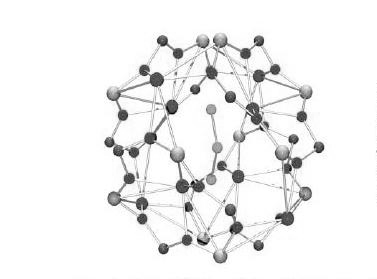
\includegraphics[width=8cm]{Sodalithkaefig.png}
 \caption{Struktur des Ultramarins.}
 \label{fig:Ultramarin}
\end{dsafigure}

Lange Zeit konnte Ultramarin nicht synthetisch hergestellt werden. Die Gewinnung aus den Lagerstätten in Chile und Afghanistan war bei geringer Ausbeute sehr zeitintensiv und aufwändig. Erst 1826 gelang Guimet die Synthese des ersten künstlichen Ultramarins. 1834 wurde die erste Fabrik eröffnet. Zur Herstellung werden Porzellanerde, Feldspat, wasserfreies Natriumcarbonat, Schwefel und ein reduzierendes Mittel verwendet. Zunächst wird die Porzellanerde bei 700$^{\circ}C$ aktiviert. Die Mischung findet danach bei 750$^{\circ}C$ statt. Dabei reagiert das Natriumcarbonat mit Schwefel und dem reduzierenden Mittel zu Natriumpolysulfid, eingelagert in die sodalithische Struktur. Damit ist die Produktion heute relativ kostengünstig und mit einer Ausbeute von 75\% blauem Ultramarin im Rohprodukt recht ertragreich. 
\cite{Buxbaum} 
\cite{Seel}

\section{Molekül- und Hybridorbitale}
\authors{Ali Serour, Johannes Wörsdörfer}
\subsection{Molekülorbitale}

Die Molekülorbitaltheorie ist eine Näherung zur quantenchemischen Beschreibung von Molekülen. Man nähert die Gesamtwellenfunktion mithilfe der Molekülorbitale an. Molekülorbitale sind Einteilchenwellenfunktionen beziehungsweise Linearkombinationen von Atomorbitalen $\chi_k$ (\ref{Linearkombination zweier Atomorbitale}):

\begin{equation}
 \label{Linearkombination zweier Atomorbitale}
 	\psi_i = \sum \limits_{k=1}^{n} c_{ik} \chi_k
\end{equation}

Dieses Verfahren wird LCAO (linear combination of atomic orbitals) genannt. Die Koeffizienten $c_{ik}$ geben an, wie stark die einzelnen Atomorbitale zu den jeweiligen Molekülorbitalen beitragen.
Es wird angenommen, dass eine chemische Bindung durch konstruktive Interferenz von Atomorbitalen beschrieben werden kann. Diese Interferenz führt zu bindenden Molekülorbitalen. Analog dazu resultieren antibindende Molekülorbitale aus destruktiver Interferenz der Atomorbitalbasis (siehe Abbildung \ref{fig:LCAO}). Die Energie bindender MOs ist niedriger als die antibindender \cite{Reinhold}.

\begin{dsafigure}
  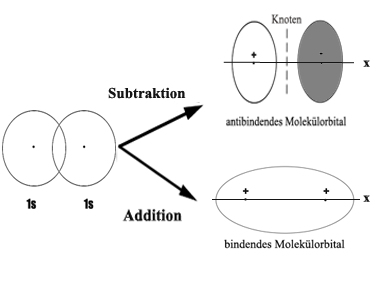
\includegraphics[width=\columnwidth]{LCAO3.png}
  \caption{Links: Linearkombination von 1$s$-Orbitalen zu $\sigma$-Molekülorbitalen. Unten rechts: Linearkombination der Atomorbitale, die zu einem bindenden Molekülorbital führt. Oben rechts: Linearkombination der Atomorbitale, die zu einem antibindenden Molekülorbital führt. }
  \label{fig:LCAO}
\end{dsafigure}

Zur Veranschaulichung bedienen wir uns des Molekülorbital-Diagramms des Wasserstoffmoleküls (siehe Abbildung \ref{fig:MO-Diagramm}).
Die beiden 1$s$-Atomorbitale der Wasserstoffatome bilden ein bindendes und ein antibindendes Molekülorbital. Die Anzahl der Molekülorbitale entspricht immer der Anzahl der Atomorbitale. Beim Besetzen der Molekülorbitale mit Elektronen werden die selben Regeln eingehalten wie im Falle von Atomorbitalen (Aufbauprinzip, Pauli-Verbot, Hundsche Regel). Die Bindungsordnung (BO) lässt sich mit der Formel
\begin{equation}
 \label{Bindungsordnung}
 	BO = \frac{n_b-n_a}{2}
\end{equation}

darstellen, wobei $n_b$ die Zahl der Elektronen in bindenden und $n_a$ die Zahl der Elektronen in antibindenden Orbitalen bezeichnet. Für das Wasserstoffmolekül ergibt sich demzufolge: $(2-0)/(2) = 1$. Somit sind die beiden Wasserstoffatome durch eine Einfachbindung gebunden.

 \begin{dsafigure}
  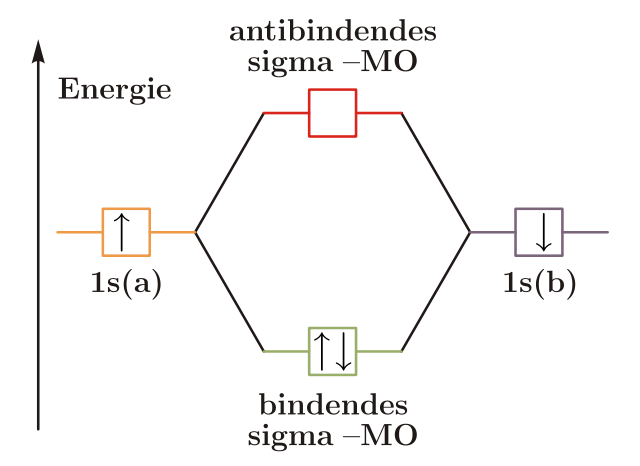
\includegraphics[width=\columnwidth]{MO-Diagramm.png}
  \caption{Molekülorbital-Diagramm des Wasserstoffmoleküls \cite{WasserstoffMO}.}
  \label{fig:MO-Diagramm}
\end{dsafigure}

Diese Einfachbindung wird als $\sigma$-Bindung bezeichnet. $\sigma$-Bindungen beziehungsweise $\sigma$-Orbitale sind rotationsymmetrisch. Das heißt, sie ändern sich durch eine Rotation um die Bindungsachse nicht (siehe Abbildung \ref{fig:LCAO}). Neben den $\sigma$-Bindungen gibt es auch $\pi$-Bindungen. Diese Bindungen beziehungsweise Orbitale sind nicht rotationssymmetrisch. Eine Rotation um 180$^\circ$ um die Bindungsachse ändert ihr Vorzeichen.

\subsection{Hybridorbitale}

Eine alternative Beschreibung der Bindungsverhältnisse bieten die Hybridorbitale. Sie können ohne großen Recheneinsatz ermittelt werden und geben ein einfaches, qualitatives Bild.
Methan hat die Form eines Tetraeders, in dem alle Wasserstoffatome den gleichen Abstand vom Kohlenstoffatom aufweisen \cite{Riedel04}. Kohlenstoff hat die Elektronenkonfiguration $2s^2 2p^2$. In der Hybridorbital-Beschreibung wird das $s$-Orbital mit den drei $p$-Orbitalen linear kombiniert, wobei vier tetraedrisch angeordnete $sp^3$-Hybridorbitale entstehen (siehe Abbildung \ref{fig:Methan}).
Die tetraedrische Geometrie des Methanmoleküls wird erzeugt, indem die 1$s$-Orbitale der Wasserstoffatome mit den $sp^3$-Hybridorbitale konstruktiv interferieren. Jedoch sind die Energien der Orbitale in diesem Modell im Gegensatz zur Molekülorbitaltheorie (siehe Abbildung \ref{fig:MO-Diagramm}) nicht definiert. 



 \begin{dsafigure}
  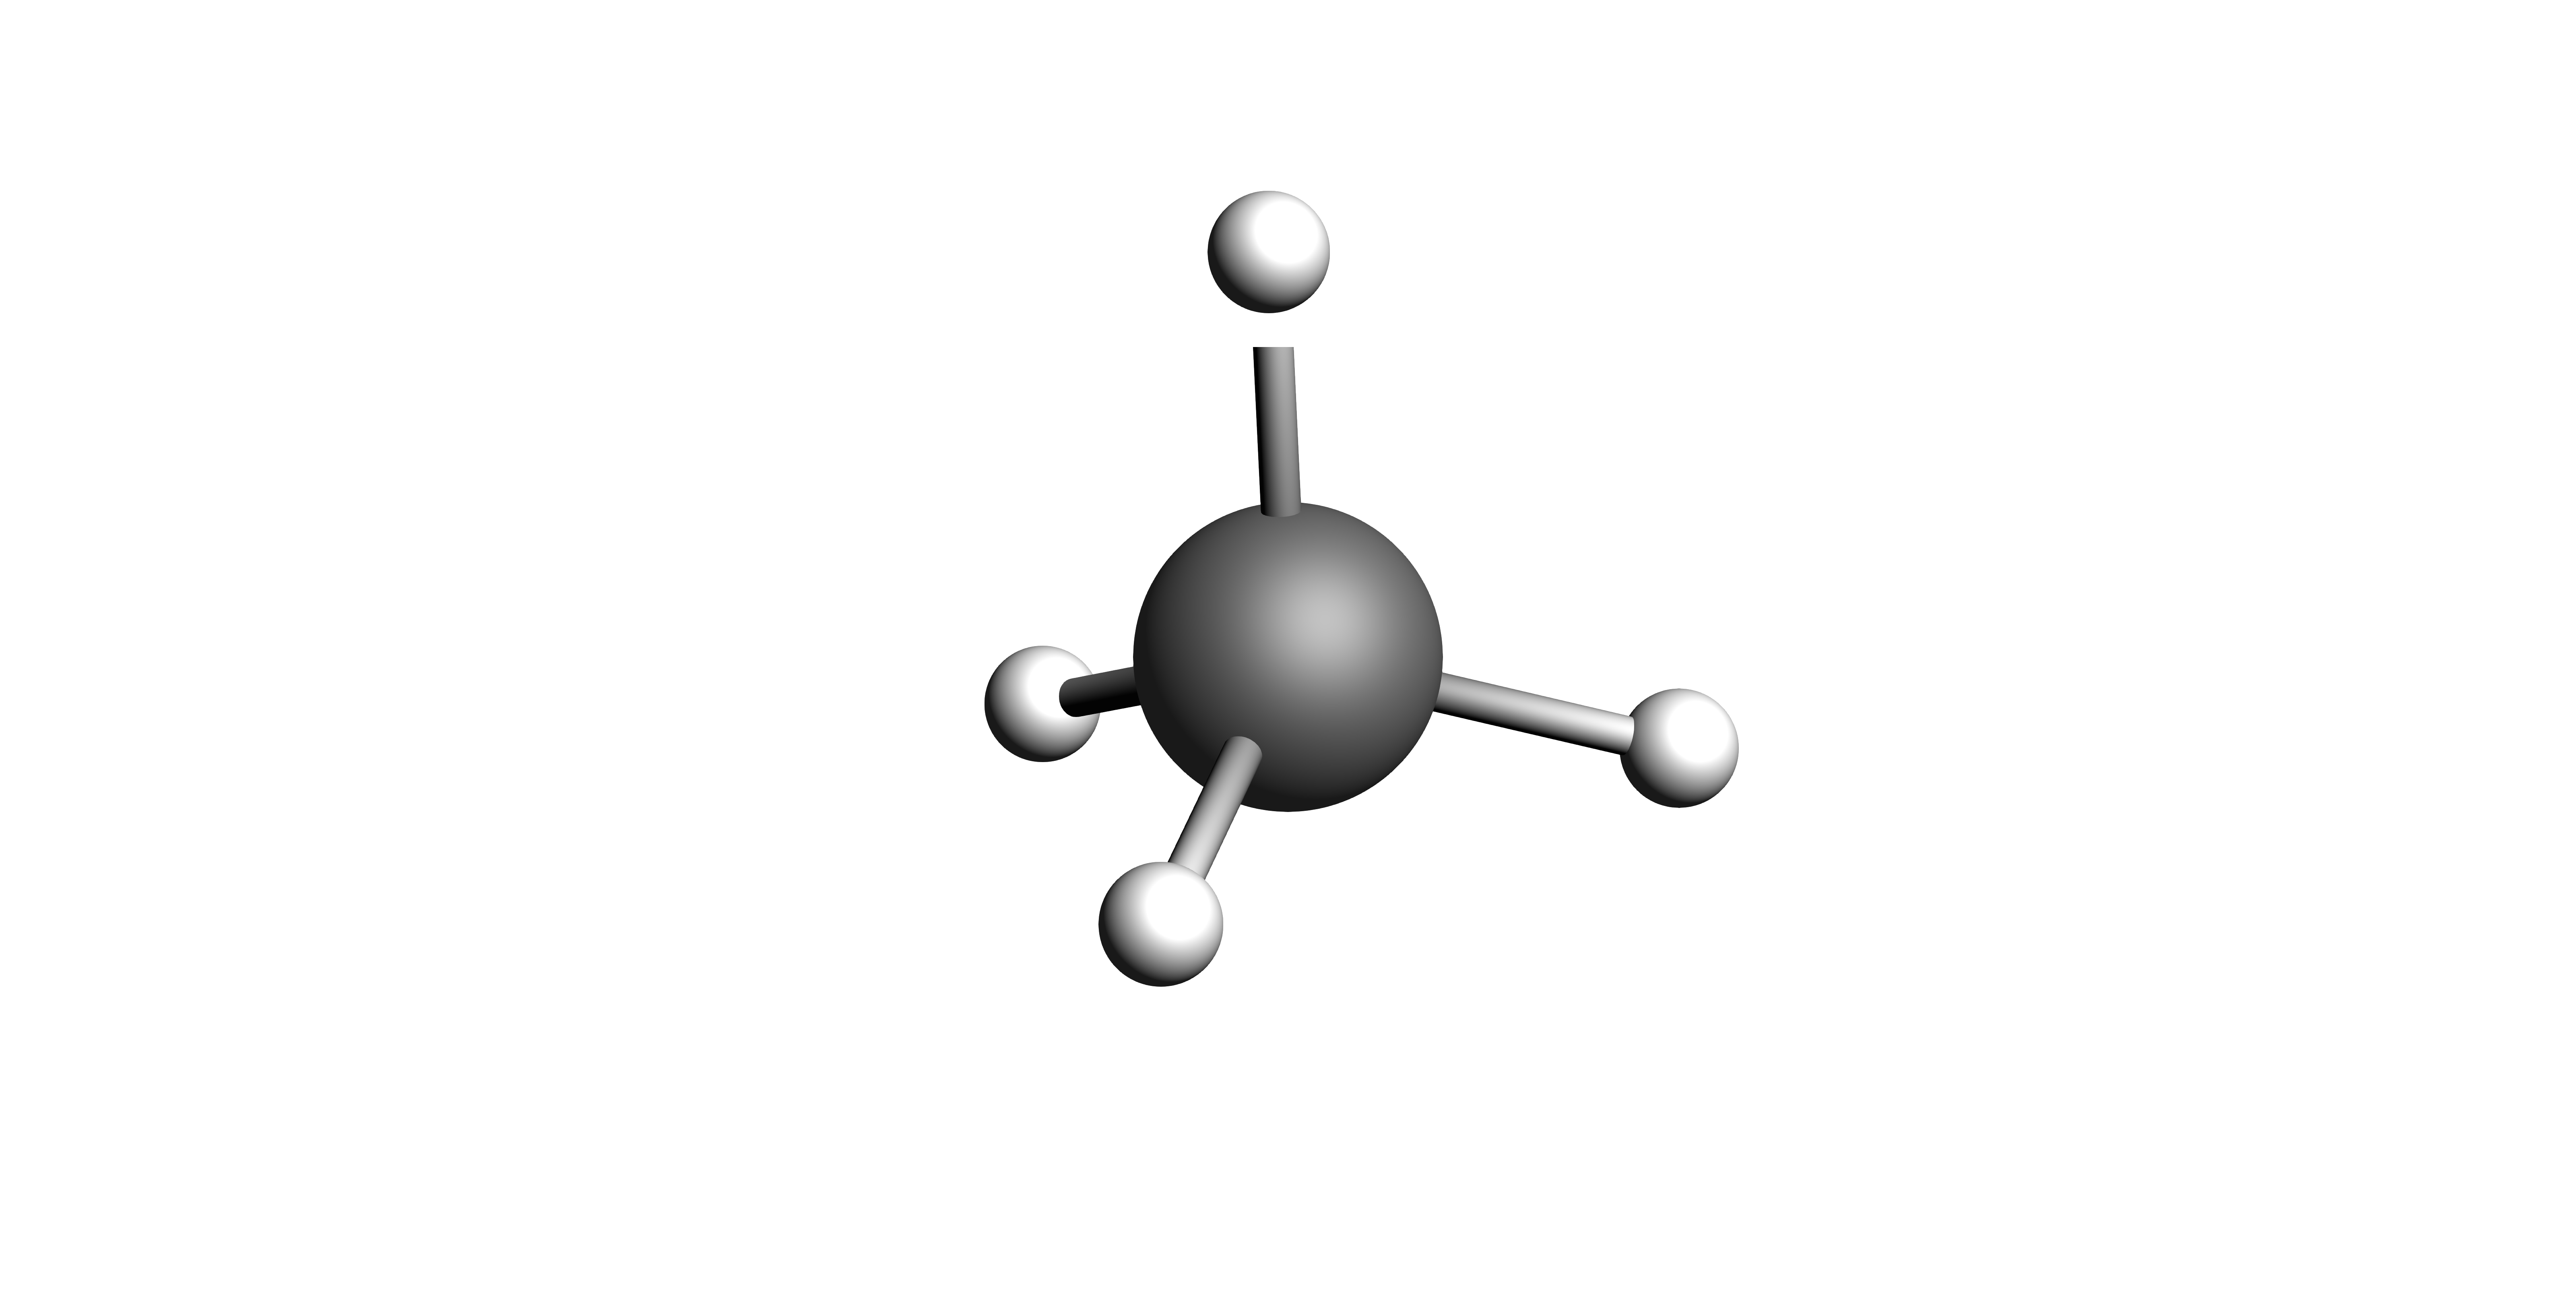
\includegraphics[width=\columnwidth]{Methan.jpg}
  \caption{3D-Modell des Methans \cite{ADF2017authors}. }
  \label{fig:Methan}
\end{dsafigure}

Des Weiteren führen die Linearkombinationen von einem $s$-Orbital und zwei $p$-Orbitalen zu drei $sp^2$-Hybridorbitalen, mit denen man die Bindungsverhältnisse im Ethen beschreiben kann. Außerdem führt eine Linearkombination von einem $s$-Orbital und einem $p$-Orbital zu zwei $sp$-Hybridorbitalen, mit denen man die Bindungsverhältnisse im Ethin beschreiben kann.

\section{Sauerstoff und Stickstoff Molekülorbitale}
\authors{David Bürg, Ole Simmering}

Im Folgenden betrachten wir das Sauerstoff- und das Stickstoffmolekül im Lichte der Molekülorbitaltheorie. Bei dieser Betrachtung fällt auf, dass die Elektronenkonfigurationen der Moleküle sich darin unterscheiden, dass die antibindenden-$ \pi $-Orbitale beim Sauerstoffmolekül [Abb. \ref{MO des O2}] einfach und beim Stickstoff [Abb. \ref{MO des N2}] unbesetzt sind. Dadurch ist das Sauerstoffmolekül paramagnetisch, hat Radikalcharakter und befindet sich zudem im Triplettzustand. Bei Stickstoff ist dies nicht der Fall. Dieser Umstand ist darauf zurück zu führen, dass das Sauerstoffatom ein Valenzelektron pro Atom mehr aufweist als das Stickstoffatom. Die gerade genannten Eigenschaften können durch eine Berechnung der Elektronenkonfiguration mit dem quantenchemischen Programm ADF \cite{ADF2017authors} feststellt werden. Die Berechnung wurde mit unrestricted DFT (DZ/B3LYP) für Sauerstoff und restricted DFT (DZ/B3LYP) für Stickstoff durchgeführt. Zuletzt wurde zur Optimierung der Struktur eine Kraftfeldoptimierung der Molekülgeometrie vorgenommen. Die Berechnung liefert die Molekülorbitaldiagramme von Sauerstoff [Abb. \ref{MO_O2_levels}] beziehungsweise Stickstoff [Abb. \ref{MO_N2_levels}].

\begin{dsafigure}
	\centering
	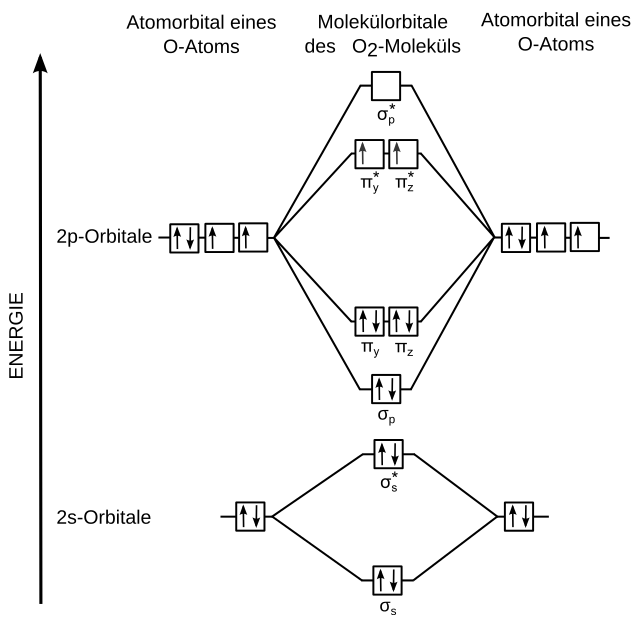
\includegraphics[width=\columnwidth]{MO_O2.png}
	\caption{Molekülorbitaldiagamm eines Sauerstoffmoleküls \cite{MOO2}.}
	\label{MO des O2}
\end{dsafigure}

\begin{dsafigure}
	\centering
	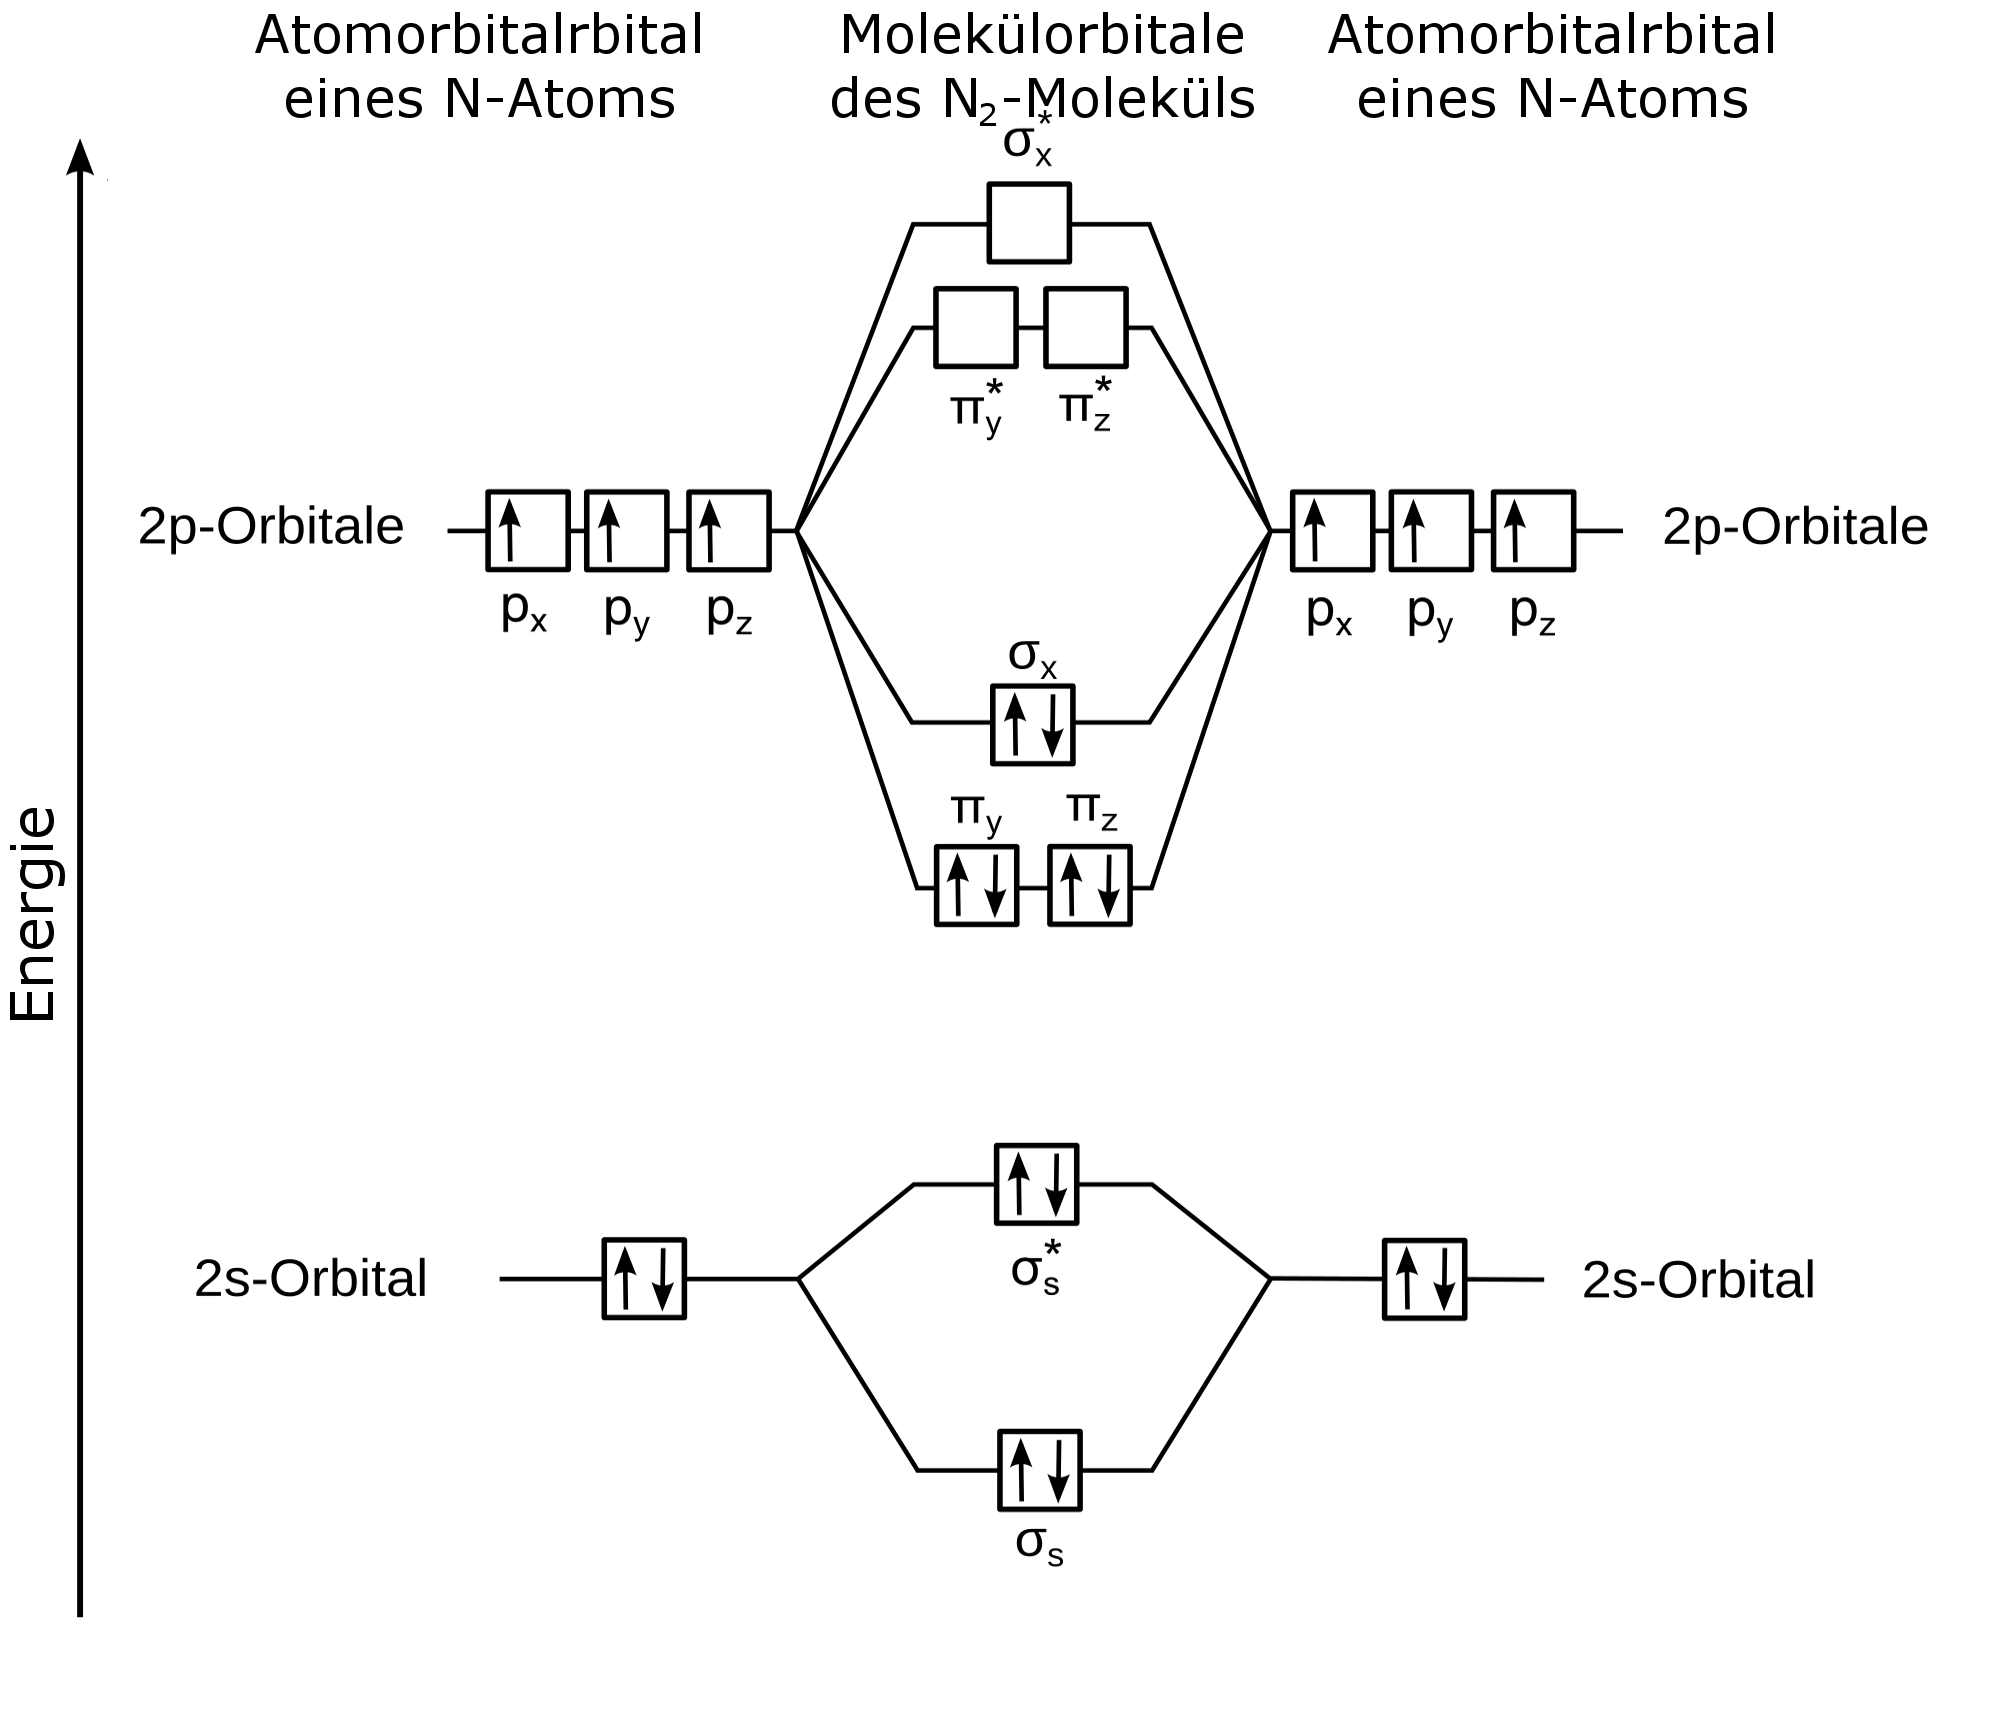
\includegraphics[width=\columnwidth]{MO_stickstoff.png}
	\caption{Molekülorbitaldiagramm eines Stickstoffmoleküls \cite{MON2}.}
	\label{MO des N2}
\end{dsafigure}

\begin{dsafigure}
	\centering
	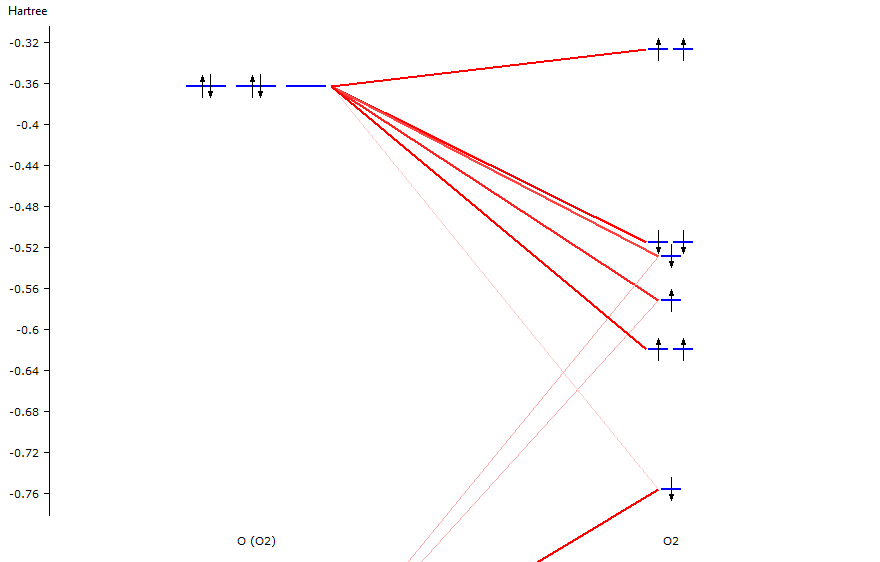
\includegraphics[width=\columnwidth]{MO_O2_levels.png}
	\caption{Mit ADF berechnetes Molekülorbitaldiagramm des Sauerstoffmoleküls.}
	\label{MO_O2_levels}
\end{dsafigure}

\begin{dsafigure}
	\centering
	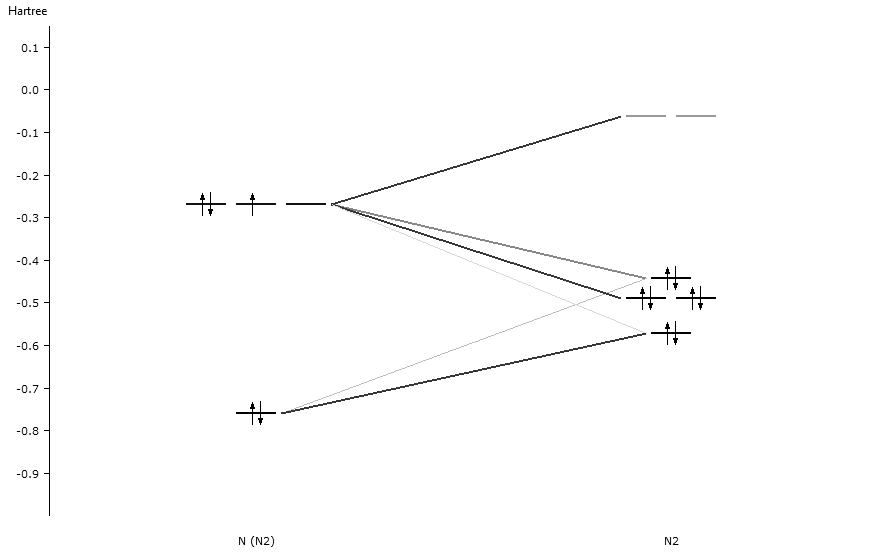
\includegraphics[width=\columnwidth]{MO_N2_levels.png}
	\caption{Mit ADF berechnetes Molekülorbitaldiagramm des Stickstoffmoleküls.}
	\label{MO_N2_levels}
\end{dsafigure}

\section{Molekülorbitale}
\authors{Isabelle Schulte-Herbrüggen, Lena Trahe, Lynn Meeder, Selin Güler}

Die Molekülorbitaltheorie wird genutzt, um die Bindungen innerhalb eines Moleküls quantenmechanisch zu beschreiben. Im Folgenden wird die Theorie auf das Ammoniak- und das Methan-Molekül angewandt.

\subsection{HOMO und LUMO -- freie Elektronenpaare}

Farbigkeit entsteht durch die Absorption von Licht bestimmter Wellenlängen. Diese Wellenlänge wiederum hängt von der Differenz der Energien der verschiedenen Zustände, die man mit den Molekülorbitalen in Näherung beschreiben kann, ab. 
Die Absorption des Lichtes kann man sich als Anregung eines Valenzelektrons in das nächsthöhere Energieniveau vorstellen. Dabei bezeichnet HOMO (Highest Occupied Molecular Orbital) das höchstgelegene besetzte Energieniveau und LUMO (Lowest Unoccupied Molecular Orbital) das nächsthöher gelegene, erste unbesetzte Energieniveau vor der Absorption. Mithilfe des ADF-Programms können sowohl Moleküle gezeichnet als auch Energien berechnet werden. Die Moleküle wurden mit DFT (DZ/B3LYP) berechnet und die Molekülgeometrie wurde mit einem Kraftfeld optimiert.

\begin{dsafigure}
	\centering
	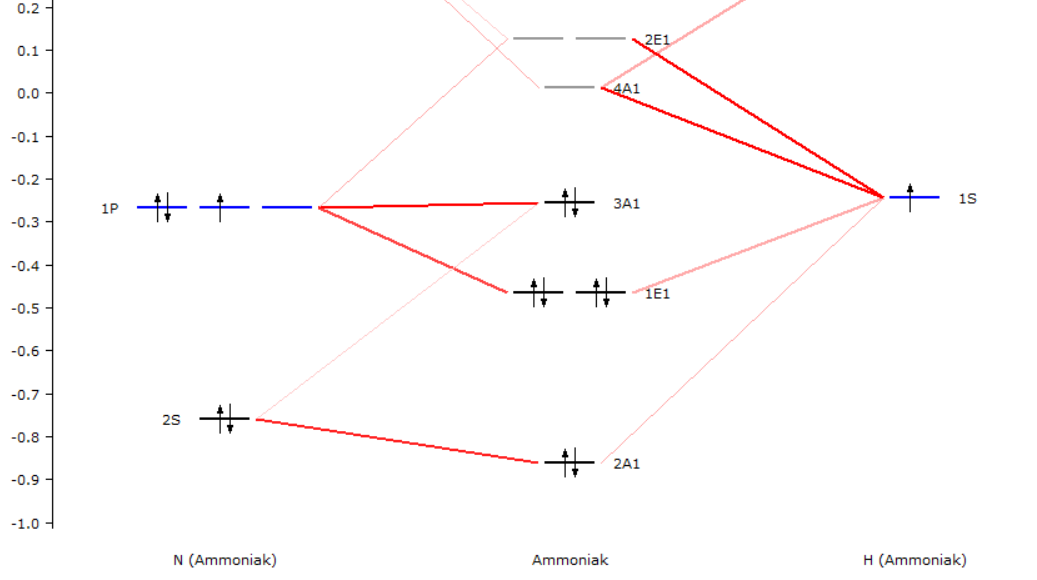
\includegraphics[width=\columnwidth]{AmmoniakLevels.png}
	\caption{Die Energieniveaus der Molekülorbitale von $NH_3$ \cite{ADF2017authors}.}
	\label{levels}
\end{dsafigure}

In Abbildung \ref{levels} sind die verschiedenen Energieniveaus der Molekülorbitale von Ammoniak dargestellt. Links sieht man die Atomorbitale des Stickstoffs, rechts sieht man die Atomorbitale des Wasserstoffs und in der Mitte befinden sich die Molekülorbitale des Ammoniaks. Abbildung \ref{homo} zeigt das höchste besetzte Orbital (HOMO), welches in diesem Fall eine $A_1$-Symmetrie aufweist. Es beschreibt das freie, nicht bindende Elektronenpaar des Ammoniaks. Das erste unbesetzte, energetisch über dem HOMO liegende Orbital ist das beim Ammoniak das ebenfalls $A_1$-Symmetrie aufweisende LUMO, welches in Abbildung \ref{lumo} dargestellt ist.

\begin{dsafigure}
	\centering
	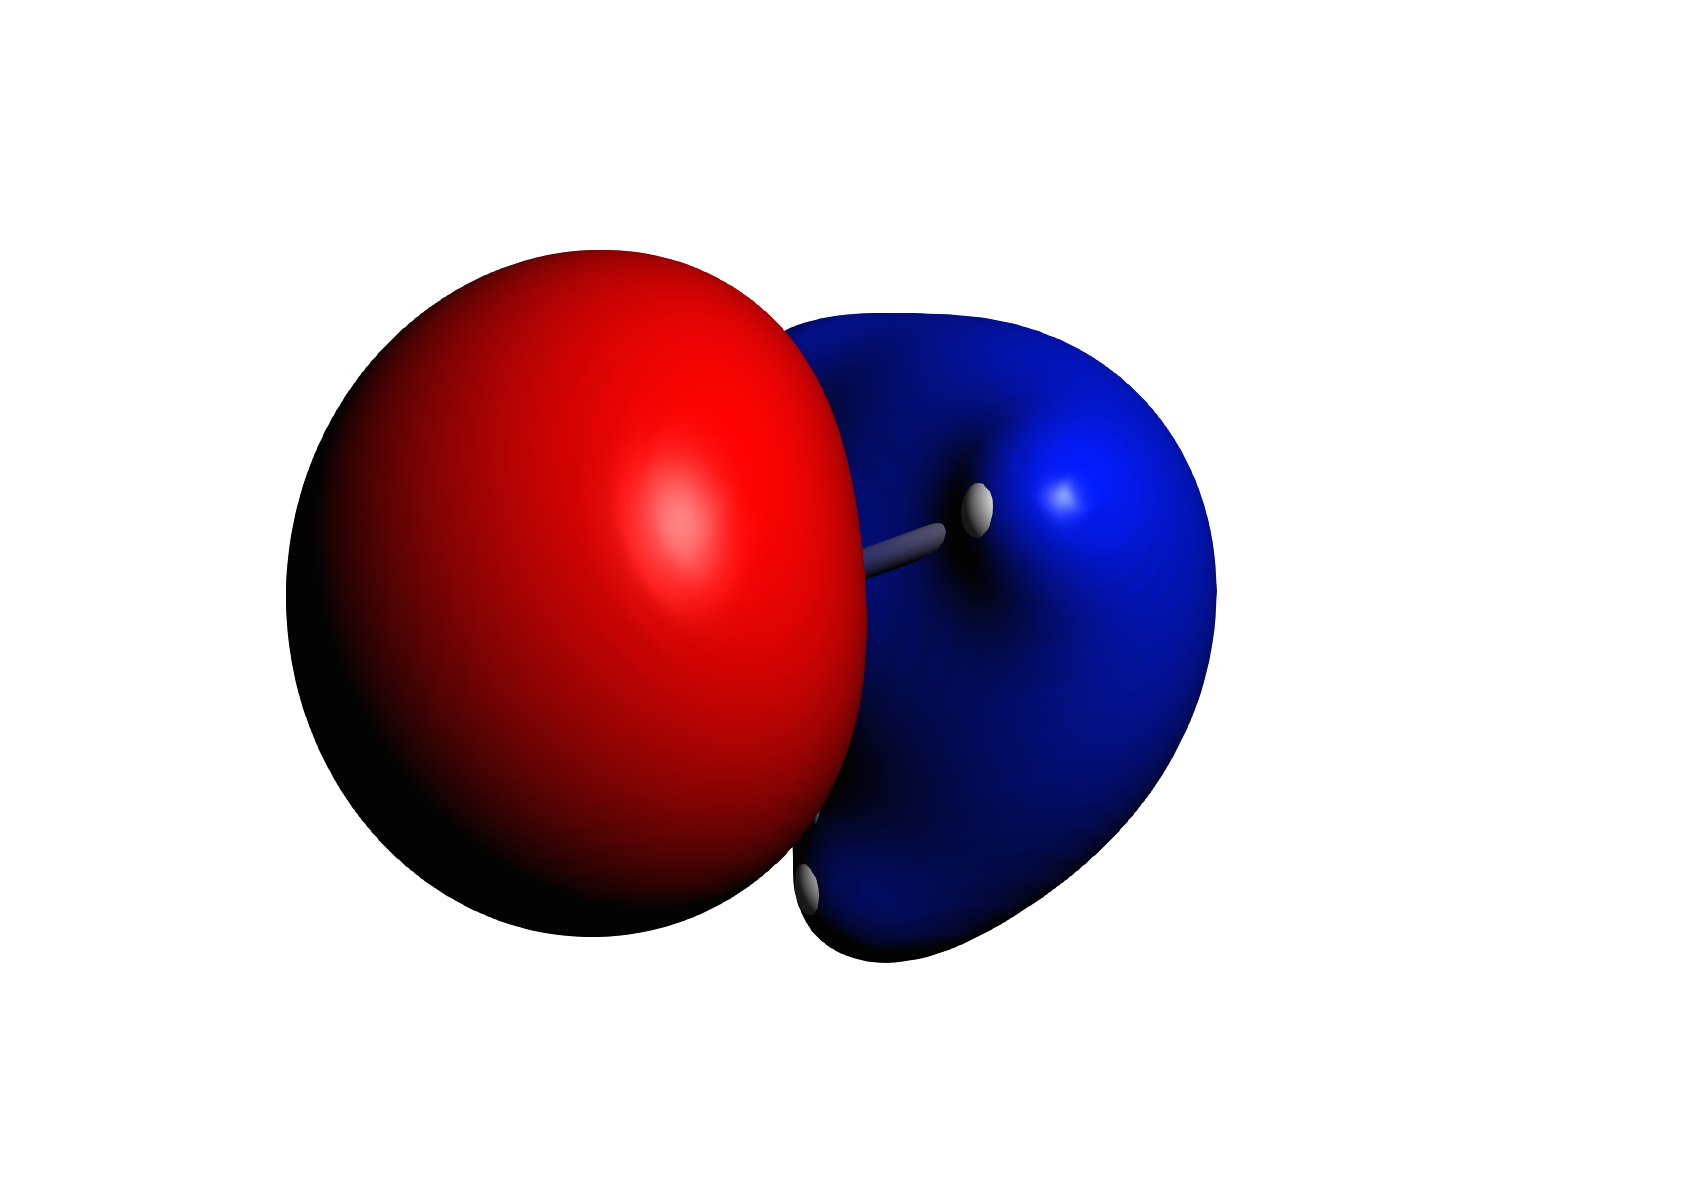
\includegraphics[width=4cm]{Orbital_3A1.png}
	\caption{HOMO des $NH_3$ \cite{ADF2017authors}.}
	\label{homo}
\end{dsafigure}

\begin{dsafigure}
	\centering
	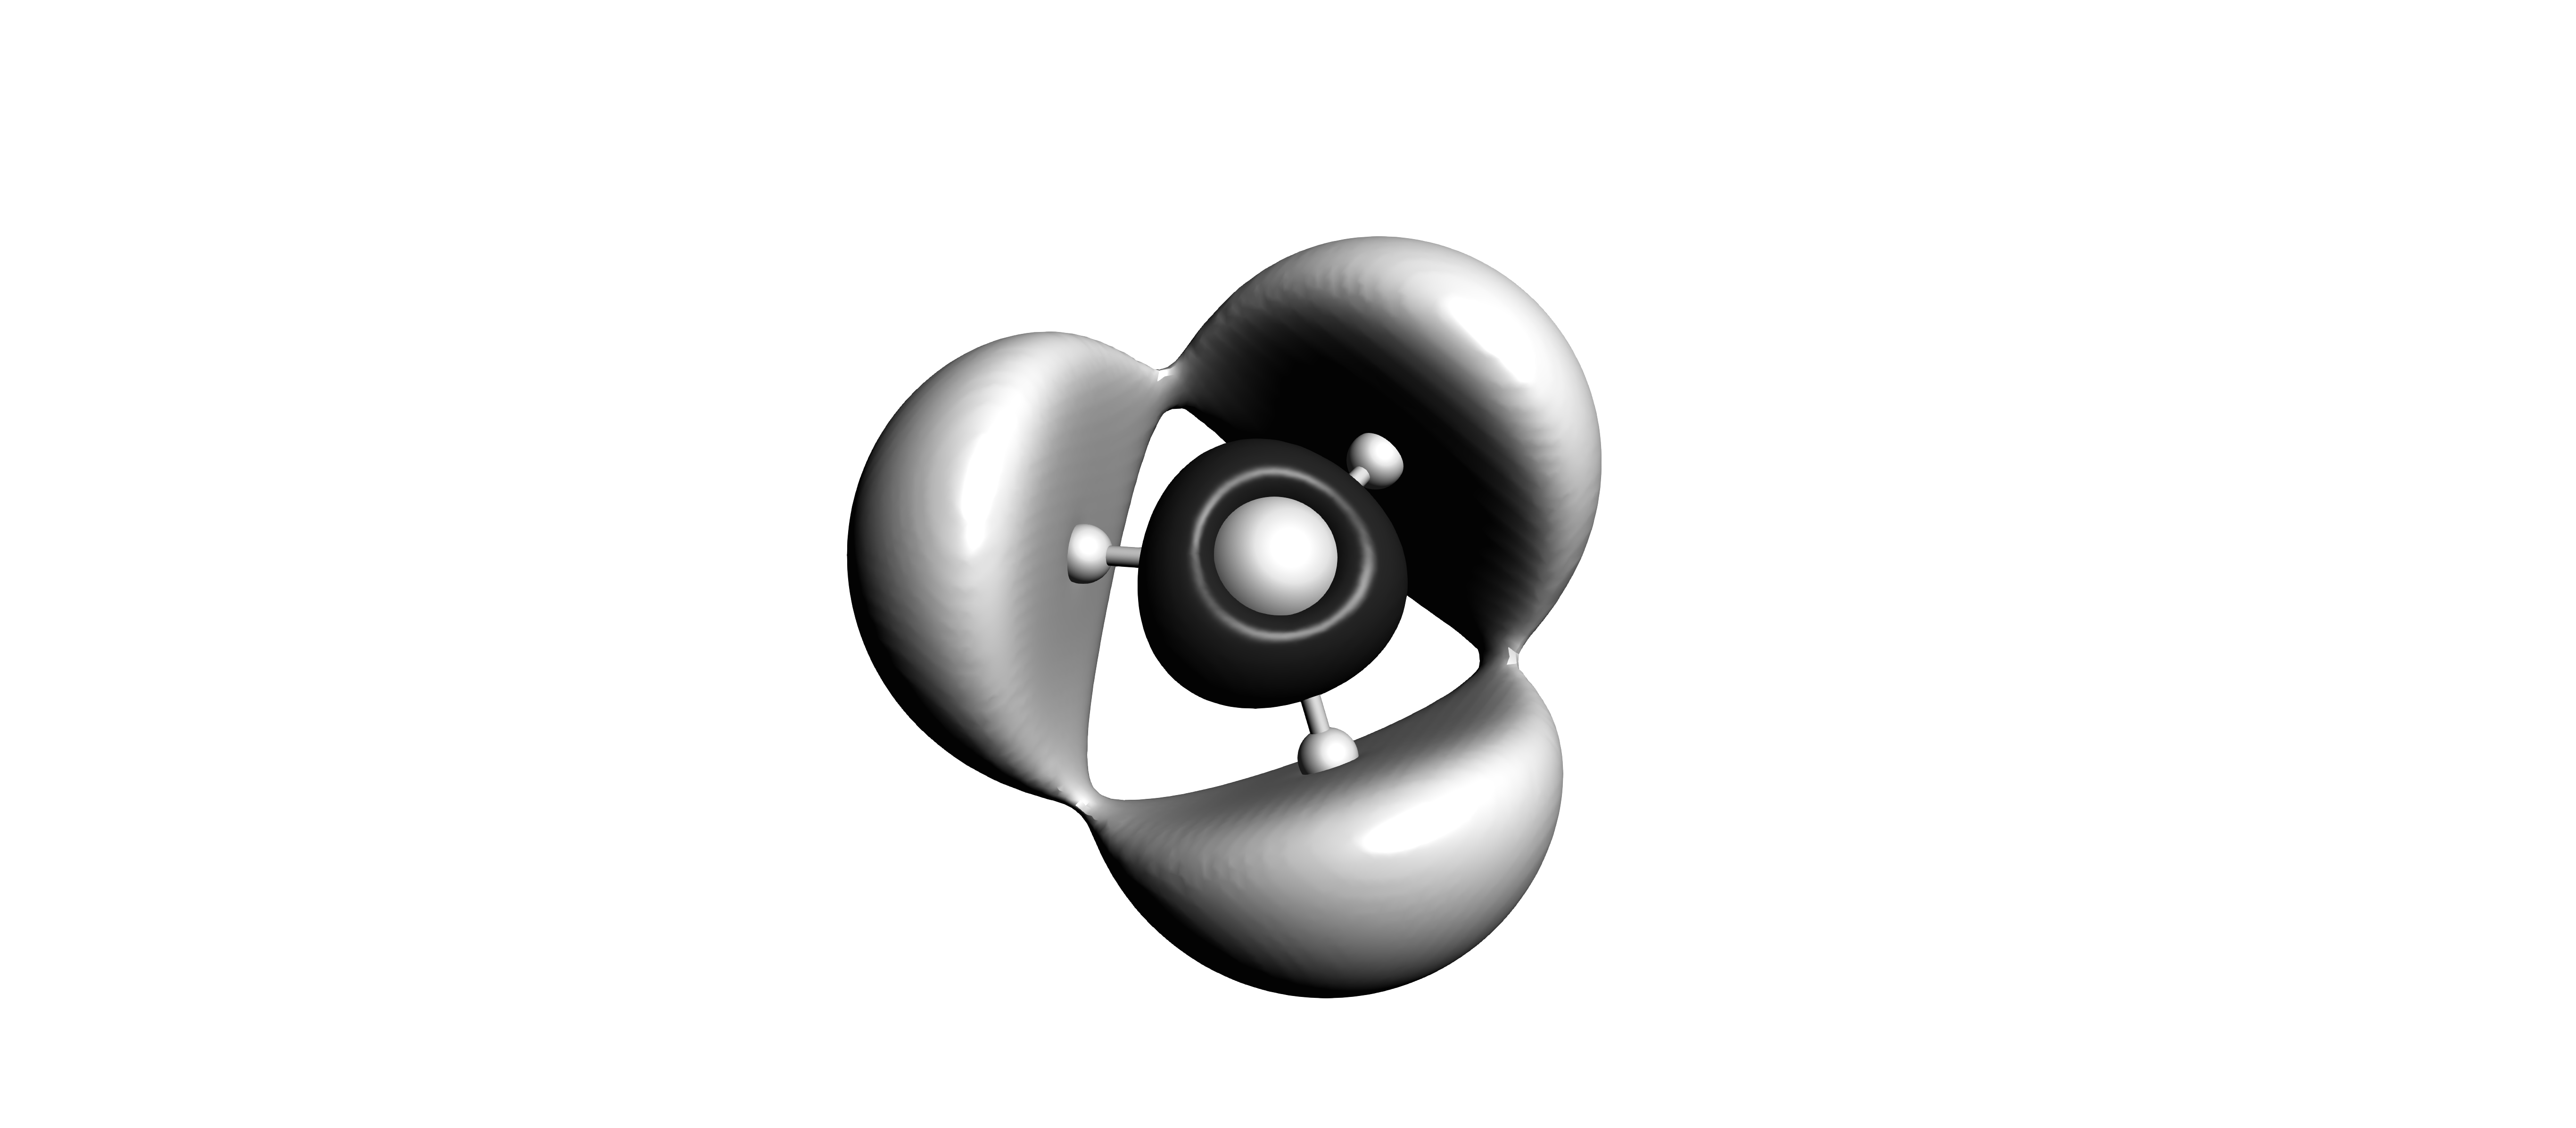
\includegraphics[width=4cm]{Orbital_4A1.png}
	\caption{LUMO des $NH_3$ \cite{ADF2017authors}.}
	\label{lumo}
\end{dsafigure}

\subsection{Hybridisierung versus Molekülorbitaltheorie}

In zahlreichen Experimenten zur Bestimmung von Winkeln und Bindungsabständen wurde belegt, dass ein Methanmolekül die Form eines Tetraeders besitzt. Alle Bindungen sind somit identisch.
Die Berechnung eines Methanmoleküls zeigte einen Unterschied zwischen den Energieniveaus der vier höchsten besetzten Molekülorbitale. Die Abbildung \ref{EnergieniveausMethan} verdeutlicht dies.

\begin{dsafigure}
 \centering
 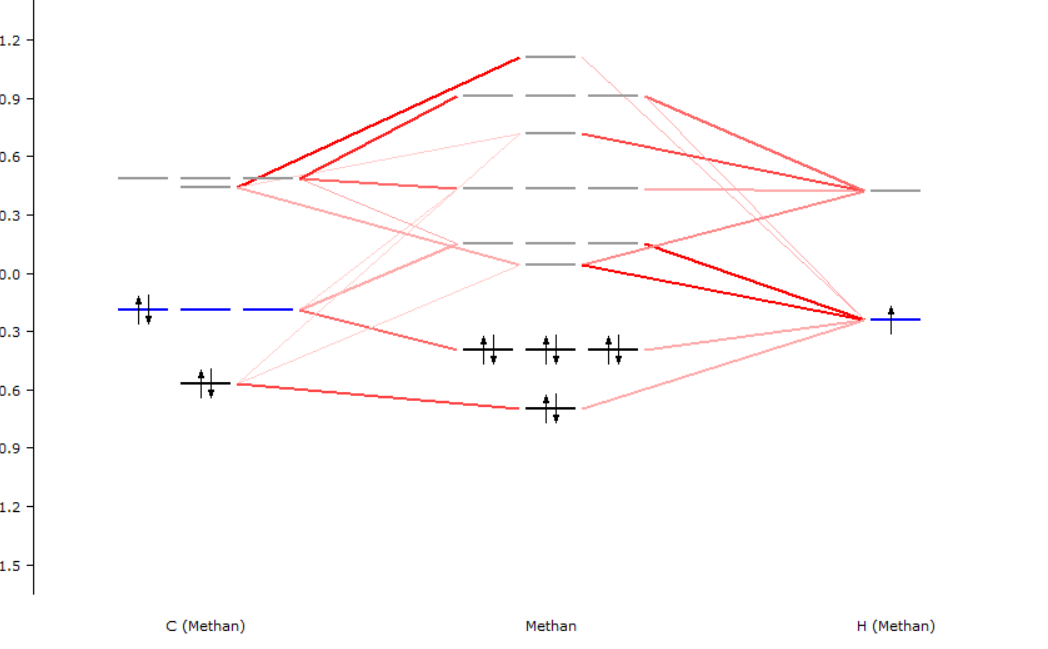
\includegraphics[width=\columnwidth]{LevelsMethan.png}
 \caption{Energieniveaus des Methanmoleküls \cite{ADF2017authors}.}
 \label{EnergieniveausMethan}
\end{dsafigure}

Links sind die Atomorbitale eines Kohlenstoffatoms und rechts die Atomorbitale eines Wasserstoffatoms abgebildet. In der Mitte sind dann die Molekülorbitale des Methanmoleküls dargestellt. Die horizontalen Linien repräsentieren die Energieniveaus der verschiedenen Orbitale. Dabei wird deutlich, dass ein Molekülorbital eine geringere Energie als die übrigen drei der vier höchsten besetzten Molekülorbitale besitzt. 
Es zeigt sich ein Unterschied zwischen dem Modell der Hybridorbitale und der von ADF genutzten Molekülorbitaltheorie, durch die man auch quantitative Informationen wie die Energien erhält. Das Modell der Hybridorbitale hingegen definiert die Energien nicht, sondern liefert qualitative Aussagen zur Geometrie und Bindungsverhältnissen. Hybridorbitale resultieren bloß aus der Anpassung der Atomorbitalbasis an die Tertaederstruktur des Moleküls. Für die Molekülorbitale werden hingegen die Energien einzelner Elektronen optimiert. 
Es handelt sich also um zwei unterschiedliche Betrachtungsweisen.
Insgesamt beschreiben beide Modelle die Struktur des Methanmoleküls als Tetraeder. In Abbildung \ref{OrbitalMethan} ist eins der drei HOMOs dargestellt.

\begin{dsafigure}
 \centering
 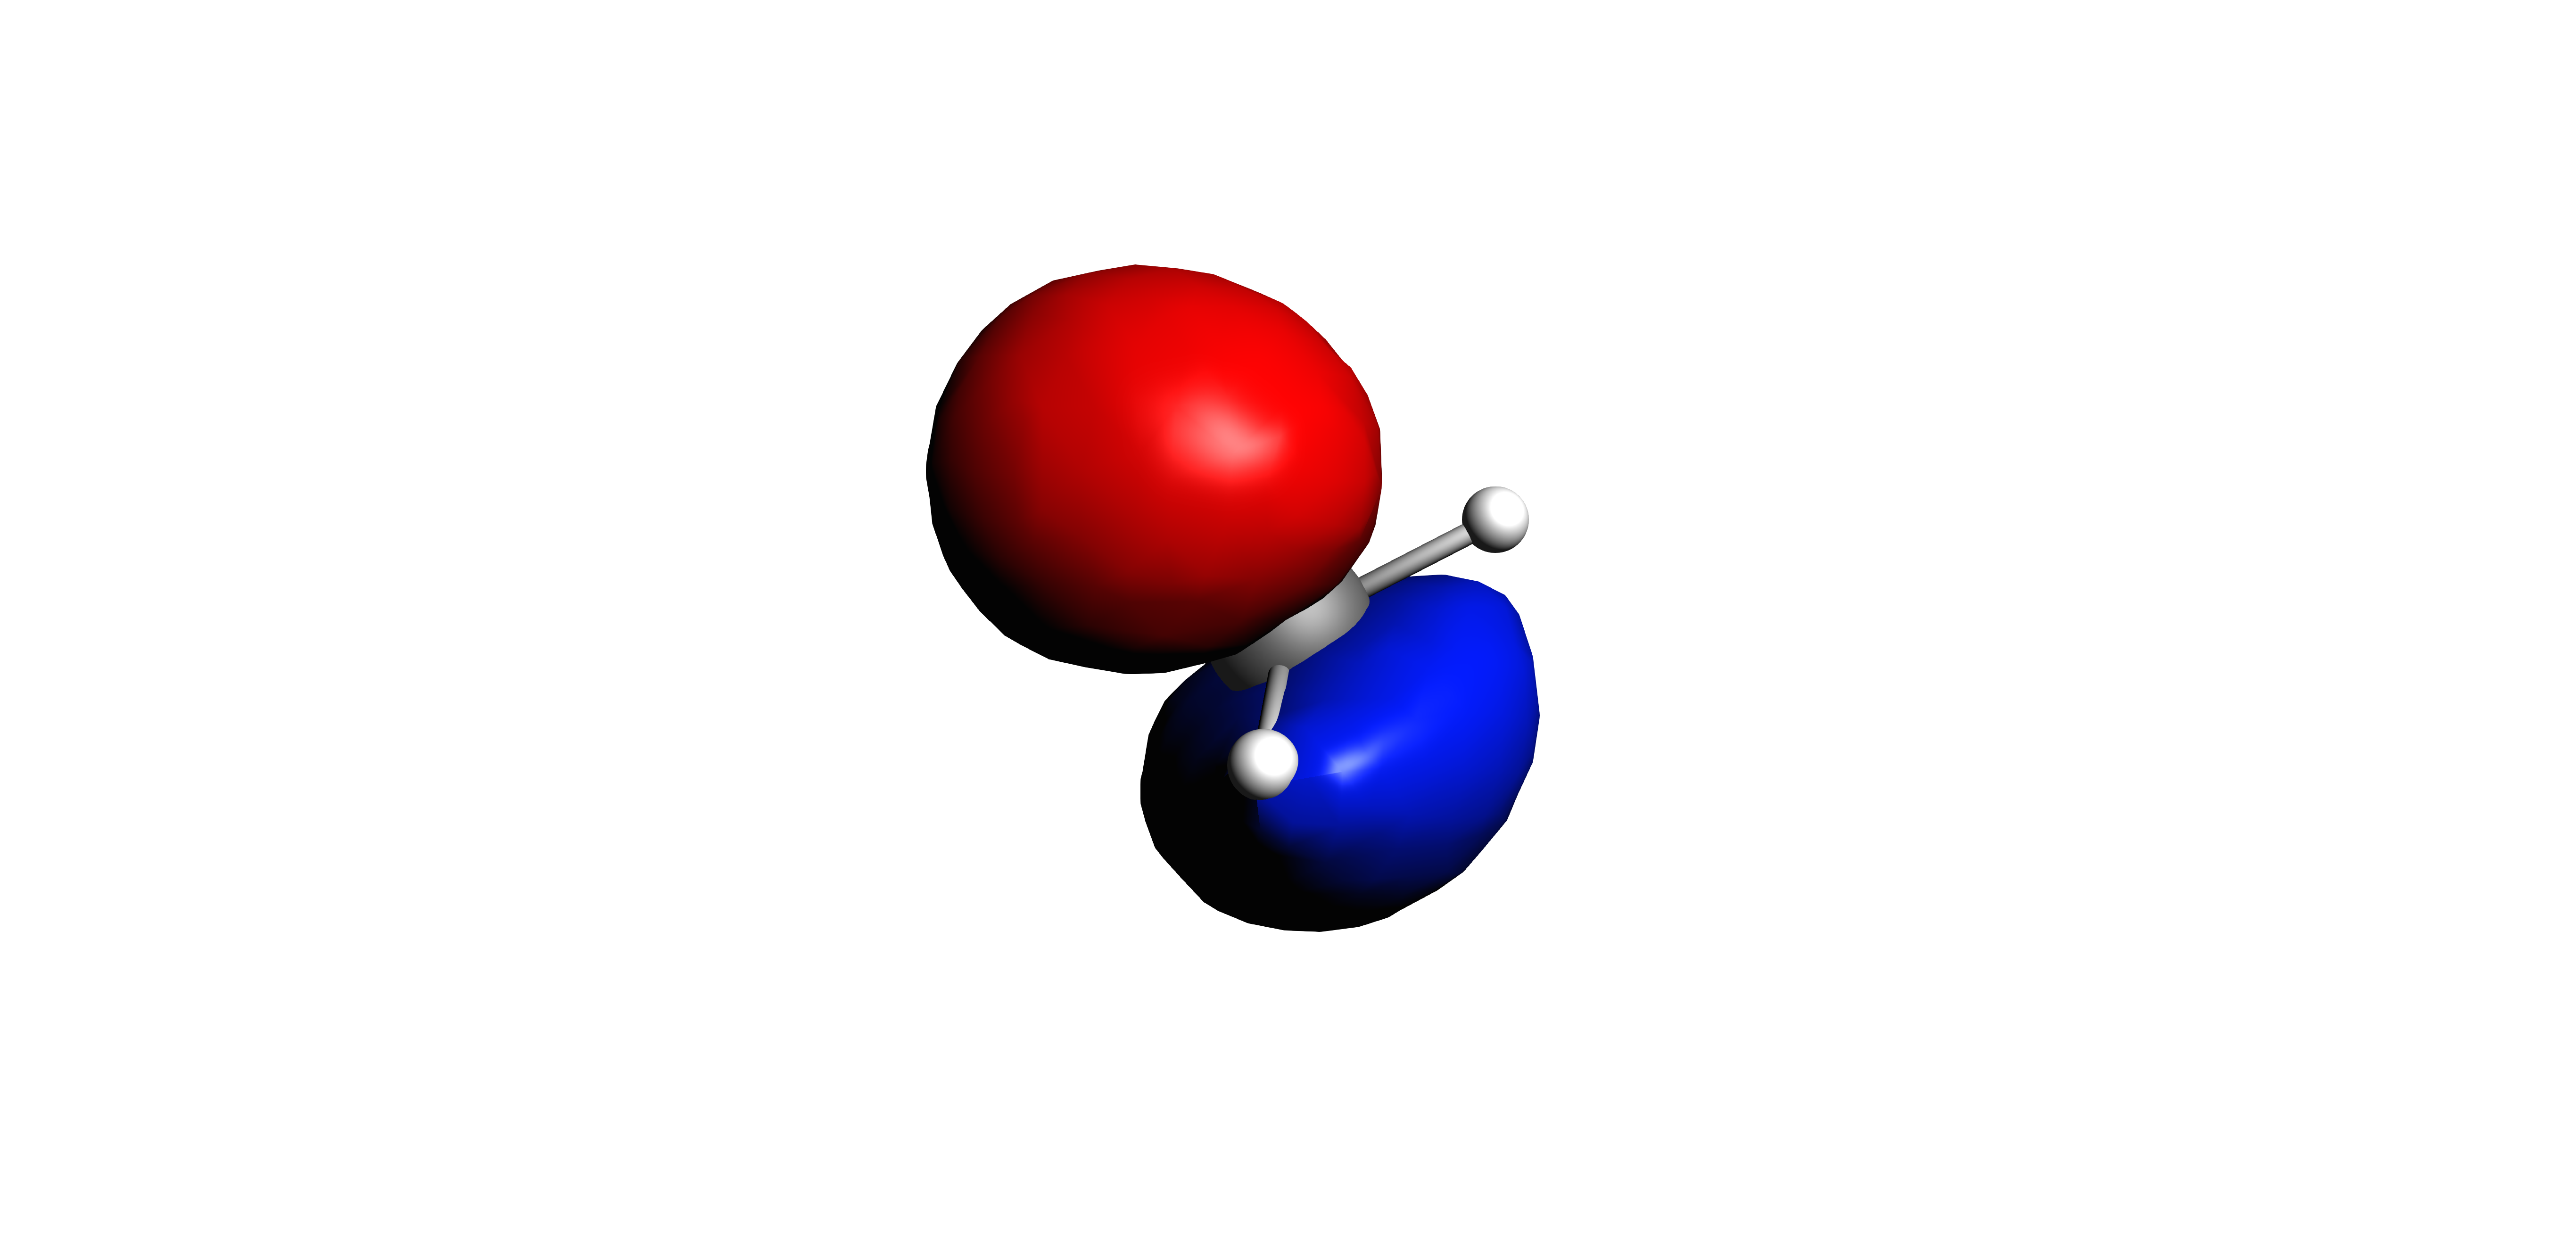
\includegraphics[scale=0.04]{MethanA5.png}
 \caption{Eines der drei HOMOs eines Methanmoleküls \cite{ADF2017authors}.}
 \label{OrbitalMethan}
\end{dsafigure}


\section{Farbe von Sulfidradikalanionen}
\authors{Johannes Wörsdörfer, Jonas Stöckmann}

Für die blaue Farben des Stoffes Ultramarin sind die Polysulfidradikalanionen $S_3 ^{-}$ und $S_4 ^{-}$ verantwortlich (siehe Ultramarin). Um ihre Farben zu bestimmen, simulieren wir mithilfe des quantenchemischen Programmpaketes ADF \cite{ADF} das Spektrum des absorbierten Lichtes (siehe Abb. \ref{fig:3s-}). Dazu verwenden wir unrestricted TDDFT (DZ/B3LYP) und die Näherung TDA. Außerdem wird eine Kraftfeldoptimierung der Molekülgeomietrie durchgeführt. Das Ergebnis der Simulation ist, dass das $S_3^{-}$-Radikalanion bei 603 nm absorbiert. Dies wäre die Wellenlänge von orangem Licht. Der Mensch nimmt die Komplementärfarbe des absorbierten Lichtes wahr. Somit hätte der Stoff die Farbe blau. Beim $S_4^{-}$ ergibt die Simulation hingegen eine absorbierte Wellenlänge von 1025 nm (siehe Abb. \ref{fig:4s-}).
Auf Basis des Modells des Teilchens im Kasten erwarten wir, dass die Energiedifferenz sich antiproportional zum Quadrat der Länge des Kastens beziehungsweise des Moleküls $L$ verhält: $\Delta E \sim \frac{1}{L^2}$ (siehe Kapitel Teilchen im Kasten). Das heißt, je länger das Molekül ist, desto kleiner sollte die Anregungsenergie und desto größer die absorbierte Wellenlänge sein. Diese grobe Abschätzung stimmt mit unserer Simulation überein, da mit zunehmender Länge der Moleküle von $S_3^{-}$ zu $S_4^{-}$ die Anregungsenergie abnimmt.


\begin{dsafigure}
 \centering
 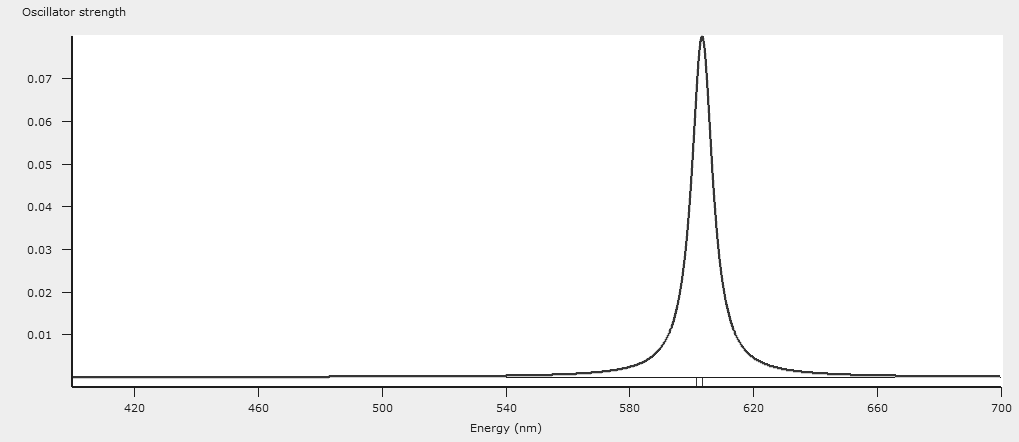
\includegraphics[width=8cm]{S3-.png}
 \caption{Spektrum eines $S_3^{-}$-Radikalanions im für den Menschen sichtbaren Bereich mit einem Peak bei ca. 603 nm.}
 \label{fig:3s-}
\end{dsafigure}

\begin{dsafigure}
 \centering
 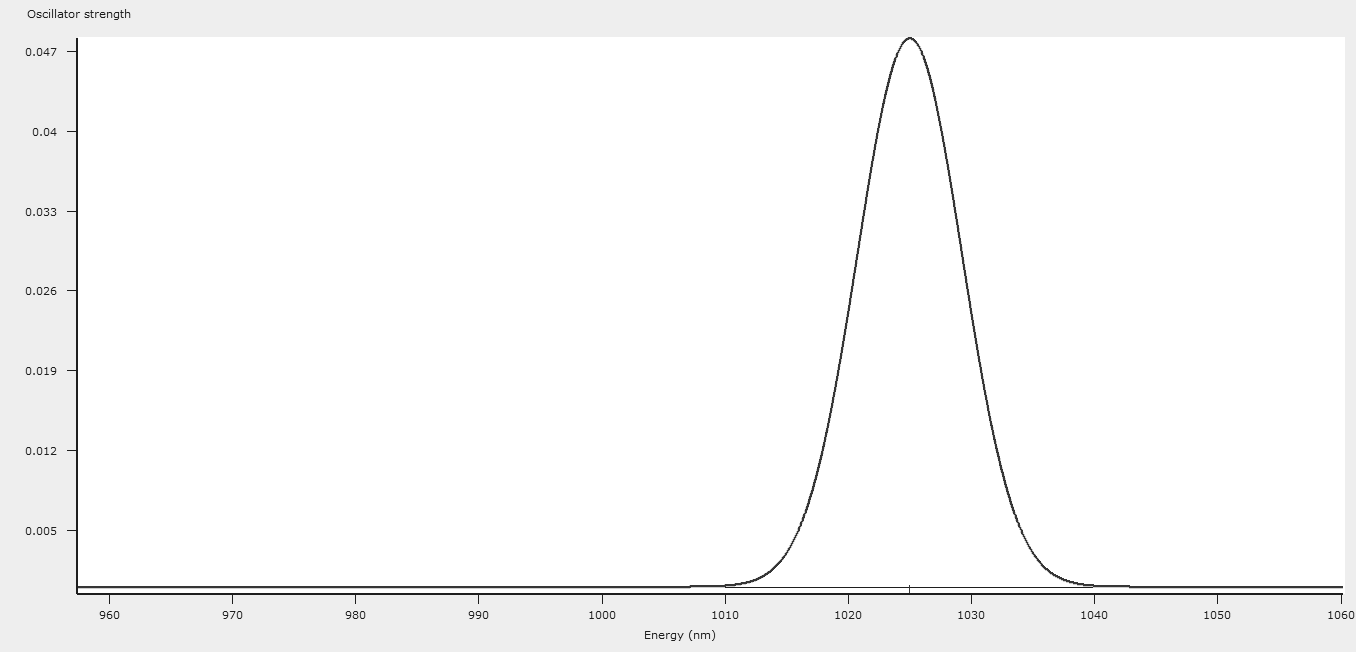
\includegraphics[width=8cm]{S4-.png}
 \caption{Spektrum eines $S_4^{-}$-Radikalanions im Bereich von 960 nm bis 1060 nm mit einem Peak bei ca. 1025 nm.}
 \label{fig:4s-}
\end{dsafigure}

\section{Ethinorbital}
\authors{Atousa Seyedian, Gala Gottschalg}
 
\begin{dsafigure}
 \centering
 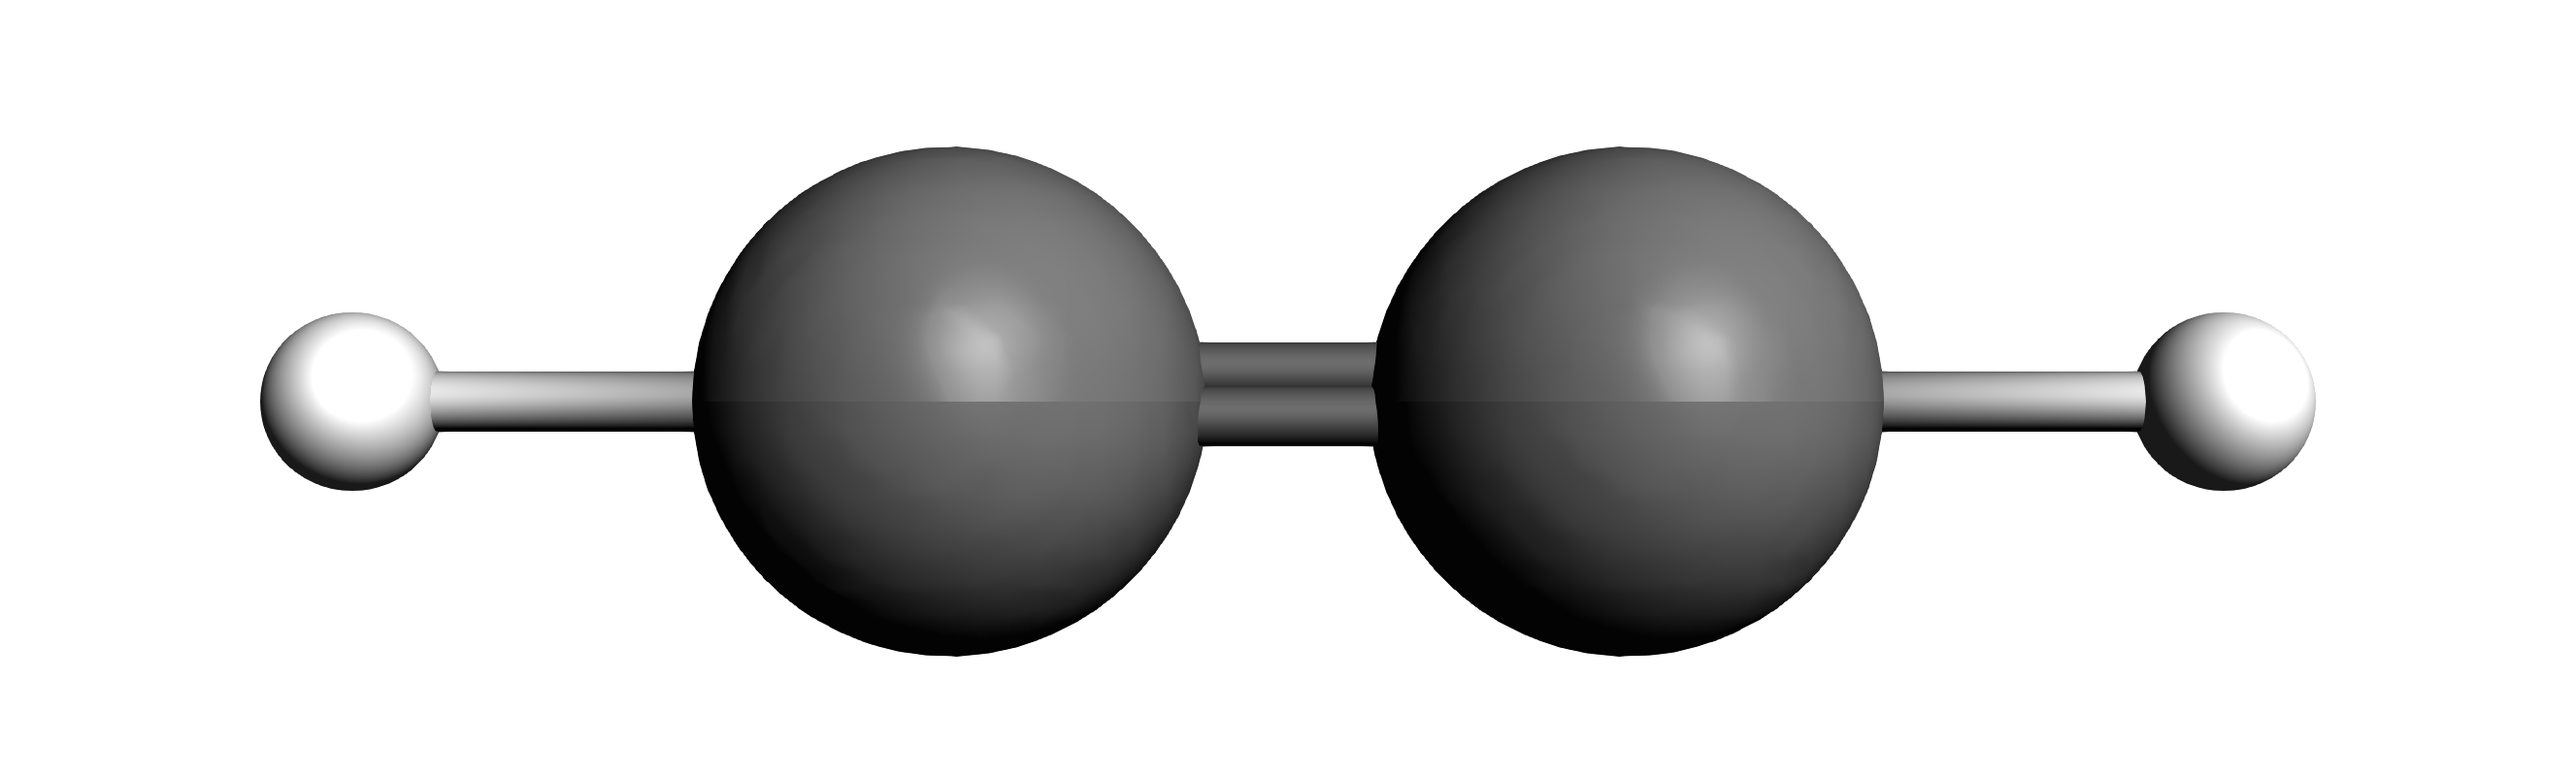
\includegraphics[width=\columnwidth]{ethin.png} 
 \caption{Molekülstruktur des Ethinmoleküls mit Dreifachbindung \cite{ADF2017authors}.}
 \label{dsafigure}
\end{dsafigure} 

Das Ethin-Molekül besitzt eine lineare Struktur. Die beiden 2$p_y$- und 2$p_z$-Orbitale stehen orthogonal zueinander und bilden zwei $\pi$-Bindungen.

\begin{dsafigure}
 \centering
 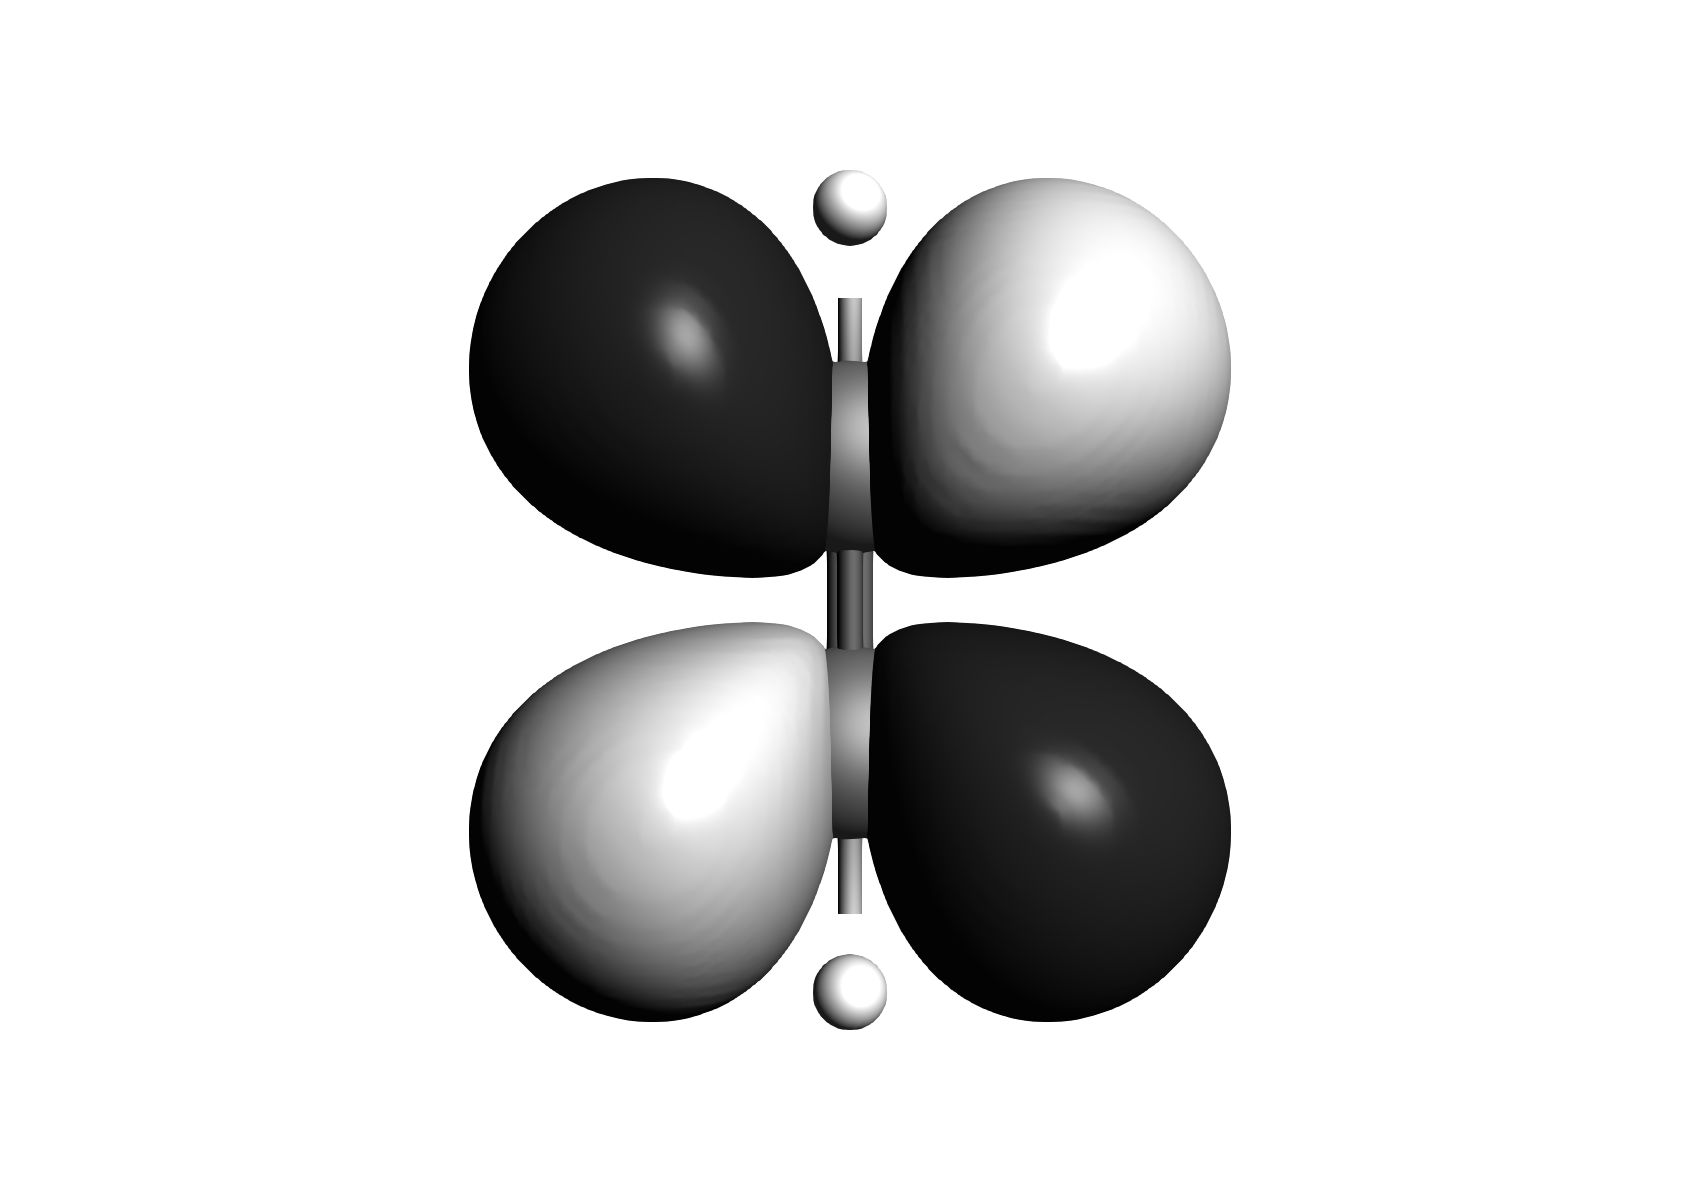
\includegraphics[width=\columnwidth]{ethin2.png}
 \caption{Ein LUMO des Ethins entlang der Bindungsachse \cite{ADF2017authors}.}
 \label{dsafigure:Ethinorbital1}
\end{dsafigure}
 
Wenn man nun die Abbildungen von HOMO und LUMO vergleicht, kann man erkennen, dass beim LUMO in Abbildung \ref{dsafigure:Ethinorbital1} eine Knotenebene orthogonal zur Bindungsachse zwischen den Kohlenstoffatomen vorhanden ist, wodurch sich das Vorzeichen ändert. Entsprechend folgt, dass das LUMO antibindend ist.

Im Modell der Molekülorbitale lässt sich die relative Bindungsstärke durch eine geringe Interferenz der $p$-Orbitale in der $\pi$-Bindung deuten.

\begin{dsafigure}
 \centering
 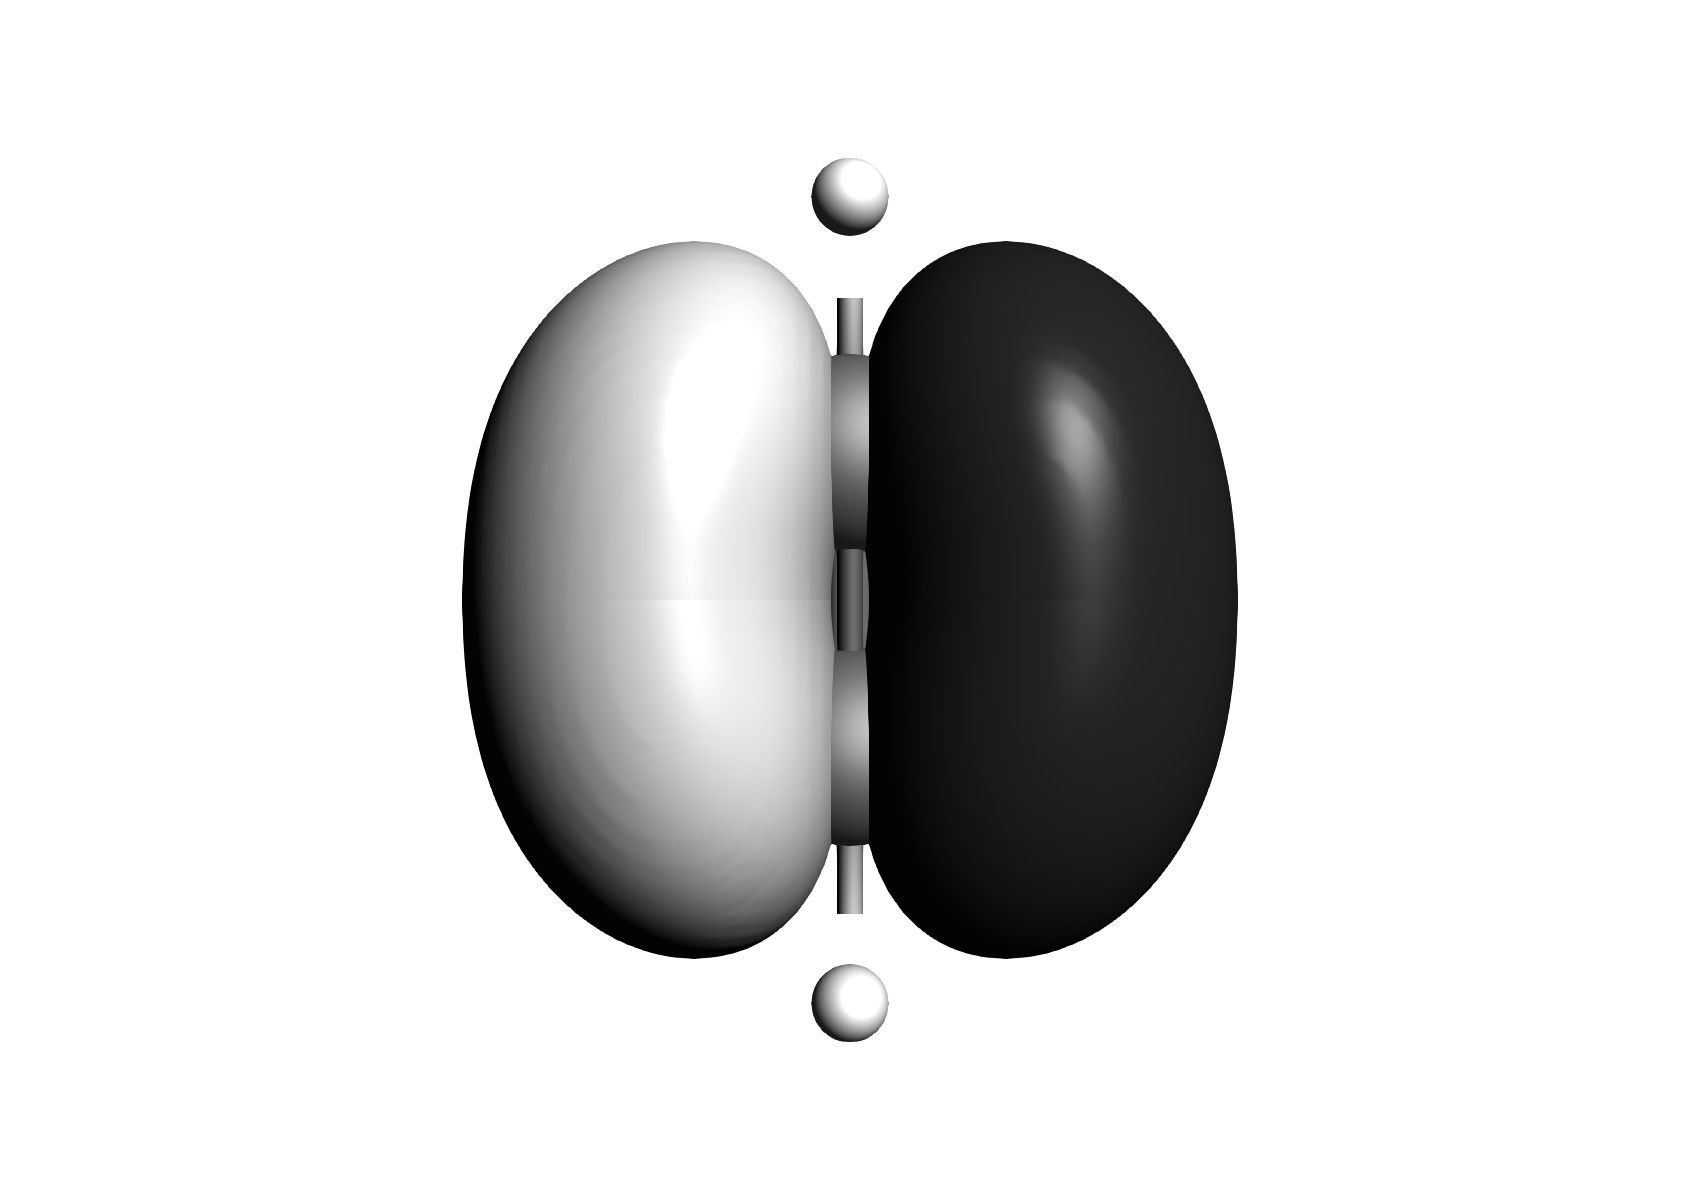
\includegraphics[width=\columnwidth]{help.png}
 \caption{Ein HOMOdes Ethins entlang derBindungsachse \cite{ADF2017authors}.}
 \label{dsafigure:Ethinorbital2}
\end{dsafigure}

Im Gegensatz dazu lässt sich beim HOMO in Abbildung \ref{dsafigure:Ethinorbital2} keine Knotenebene ausmachen, da sich das Vorzeichen nicht ändert und das HOMO bindend ist.
Alle Abbildungen wurden mit dem quantenmechanischen Programm ADF erstellt. Die Molekülorbitale sind mit DFT (DZ/B3LYP) berechnet worden, nachdem die Molekülgeometrie mit einem Kraftfeld optimiert wurde.

\section{Indigo}
\authors{Kristina Heuser, Lena Trahe}

Der Farbstoff Indigo, der in einem intensiven dunkelblau/violett erscheint, kann aus der indischen Indigofera Pflanze, dem Färbewaid oder dem Färbeknöterich, wie bereits im Altertum, natürlich oder mit Hilfe der Heumann-Synthesen auf künstliche Weise gewonnen werden \cite{Schmidt,Steingruber}. Die erste Totalsynthese des Indigos aus Isatin, welches aus Phenylessigsäure dargestellt wurde, gelang 1878 dem Chemiker Adolf von Baeyer. In zwei weiteren wirtschaftlichen Syntheseverfahren wird Phenylglycin, welches aus Anilin, oder Phenylglycin-o-carbonsäure, welches aus Anthranilsäure hergestellt wird, mit Kaliumhydroxid zu Indoxyl verschmolzen (siehe Abb. \ref{fig:HeumannSynthese}). Indoxyl oxidiert weiter zu Indigo.

\begin{dsafigure}
 \centering
 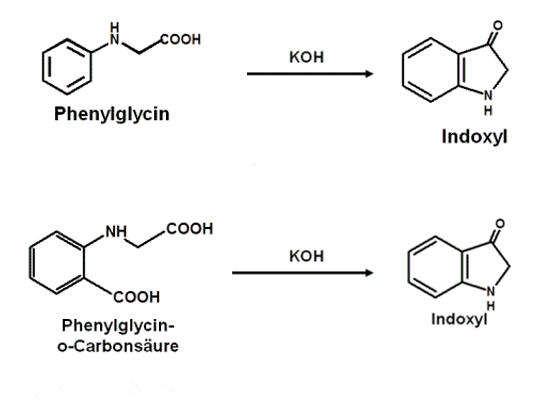
\includegraphics[width=\columnwidth]{HeumannSynthese.png}
 \caption{Heumann Synthesen des Indoxyls beziehungsweise Indigos \cite{HeumannSynthese}.}
 \label{fig:HeumannSynthese}
\end{dsafigure}

Der Farbstoff ist von wirtschaftlicher Bedeutung, da dieser in großen Mengen genutzt wird, um Textilien und Denim-Stoffe einzufärben. Dabei wird das zu verwebende Garn oder der Stoff in eine Leuko-Indigo-Lösung gegeben. Das Leuko-Indigo oxidiert an der Luft zum wasserunlöslichem, blauen Indigo (siehe Abb. \ref{fig:Reduktion}).

\begin{dsafigure}
 \centering
 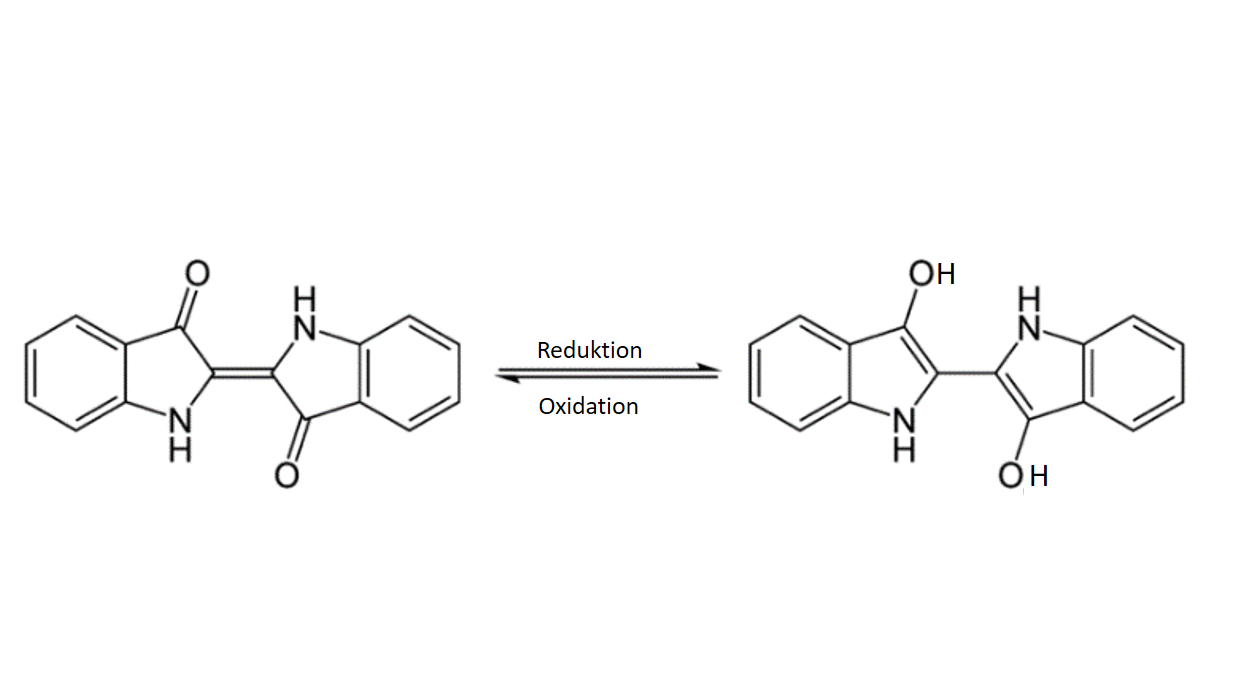
\includegraphics[width=\columnwidth]{Reduktion_Indigo.png}
 \caption{Reduktion des Indigos zu Leuko-Indigo und Oxidation des Leuko-Indigos zu Indigo \cite{Indigo_Reduktion}.}
 \label{fig:Reduktion}
\end{dsafigure}

Indigo hat die Summenformel $C_{16}H_{10}N_{2}O_{2}$ und besitzt zwei Carbonyl-Gruppen, welche durch die Reduktion protoniert und zu Hydroxyl-Gruppen werden.
Die Löslichkeit des Leuko-Indigos in Wasser lässt sich durch die entstandenen Hydroxyl-Gruppen erklären, da diese Wasserstoffbrückenbindungen eingehen können.
Der Wechsel der Farbe von gelb zu blau bei der Oxidation des Leuko-Indigos ist auf die Veränderung des $\pi$-Systems zurückzuführen.
 

\section{Hückeltheorie}

Autoren: David Bürg, Isabelle Schulte-Herbrüggen

Die Hückeltheorie wurde in den 1930er Jahren von Erick Hückel entwickelt. \cite{Reinhold} Sie erlaubt eine einfache Beschreibung von konjugierten Doppelbindungssystemen. Die Methode arbeitet mit vielen Näherungen. Daher ist sie zwar ungenau, aber einfach anzuwenden. Sie baut auf der Näherung von $\pi$-Molekülorbitalen und deren Energien über Linearkombinationen von p-Atomorbitalen auf. Die Linearkombinationen können mit:

\begin{align}
 \psi_{i} = \sum \limits_{k=1}^n c_{ik} \chi_k 
\end{align}

beschrieben werden. Der Koeffizient $c_{ik}$ gibt hierbei an, wie  stark die einzelnen Atomorbitale $\chi_k$ am Molekülorbital $\psi_i$ beteiligt sind. Die Koeffizienten $c_{ik}$ lassen sich über die Summen:

\begin{align}\label{eq:hueckel}
  \sum \limits_{k=1}^n (H_{jk}-\epsilon_i S_{jk}) c_{ik} = 0
\end{align}

bestimmen. $H_{jk}$ ist das Hamiltonmatrixelement, $S_{jk}$ das Überlappmatrixselement und $\epsilon_i$ ist die Energie des Molekülorbitals. Mit Gleichung (\ref{eq:hueckel}) kann nun die Hückelmatrix formuliert werden. Dabei wird angenommen, dass die Hamiltonmatrixelemente aller Kohlenstoffatome gleich sind, sowie dass die Wechselwirkungen aller nächsten Nachbarn gleich sind. Zusätzlich vereinfacht man die Beschreibung noch weiter, indem die Wechselwirkungen zwischen nicht-nächsten Nachbarn komplett vernachlässigt werden. Aufgrund dieser Vereinfachungen sind die Ergebnisse, die man durch Anwenden der Hückeltheorie erhält, grobe Näherungen.


Indem man fordert, dass die Determinante der Hückelmatrix verschwindet, erhält man einen Satz gekoppelter Gleichungen, deren Lösung die Koeffizienten $c_{ik}$ und die Orbitalenergien $\epsilon_i$ liefert. So kann nun die Energiedifferenz zwischen HOMO und LUMO mit:

\begin{align}
  \Delta E = \epsilon_{LUMO} - \epsilon_{HOMO}
\end{align}

berechnet werden. Diese Energiedifferenz erlaubt eine grobe Abschätzung der ersten Anregungsenergie des Moleküls.

Beschreibt man das 1,3-Butadien-Molekül mit der Hückelthoerie, erhält man die in Abbildung  \ref{fig:Hueckel_Butadiene} dargestellten Molekülorbitale.

\begin{dsafigure}
 \centering
 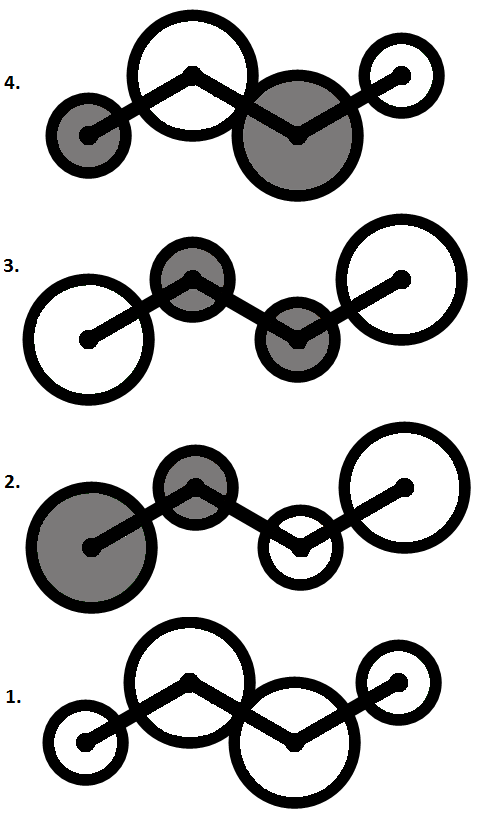
\includegraphics[width=8cm]{Hueckel_Butadiene.png}
 \caption{Aufsicht auf ein 1,3-Butadienmolekül. Schematische Darstellung der Hückelmolekülorbitale von 1,3-Butadien.}
 \label{fig:Hueckel_Butadiene}
\end{dsafigure}

Die Radien der Kreise entsprechen den Koeffizienten $c_{ik}$, während Weiß und Grau die Positivteile beziehungsweise Negativteile beschreiben. Das erste Orbital ist das energetisch günstigste Molekülorbital von Butadien, da es nur bindende Wechselwirkungen aufweist und keine Knotenebene besitzt; es ist ein bindendes Orbital. Das zweite Orbital hingegen weist zwei bindende Wechselwirkungen und eine Knotenebene auf. Es handelt sich auch hier um ein bindendes Orbital. Beim dritten un vierten Orbital handelt es sich um antibindende Orbitale. Das dritte Orbital zeigt zwei Knotenebenen und eine bindende Wechselwirkung und das vierte Orbital weist drei Knotenebenen und keine bindenden Wechselwirkungen auf. Sie haben also mehr Knotenebenen als bindende Wechselwirkungen. Die Energie vier Molekülorbitale nimmt in aufsteigender Reihenfolge zu.

\section{Koordinationsverbindungen I -- Kristallfeldtheorie}
\authors{Isabelle Schulte-Herbrüggen, Jonas R. Stöckmann}
\subsection{Allgemeines}

Die Koordinationsverbindungen wurden 1893 von Alfred Werner erstmals konsistent beschrieben. 
\cite{Werner1893}
Sie bestehen aus einem Zentralatom, welches sich in der Mitte des Komplexes befindet und von Liganden umgeben ist.
 Bei Liganden handelt es sich um Moleküle oder Anionen mit mindestens einem freien Elektronenpaar. Die Koordinationszahl des Komplexes gibt die Anzahl der Liganden beziehungsweise die Anzahl der an das Zentralatom koordinativ bindenden 
Haftatome der Liganden an. 
Diese Aussage konnte mithilfe experimentell ermittelter Werte der molaren Leitfähigkeit unterschiedlicher Komplexe getroffen werden.
So hat NaCl eine molare Leitfähigkeit von 123 $\frac{cm^3}{\Omega*mol}$, bei einem freien Chloridion. $CoCl_3\cdot5NH_3$ hat eine molare Leitfähigkeit von 261$\frac{cm^3}{\Omega*mol}$, was auf zwei freie Chloridionen schließen lässt. Daraus kann man folgern, dass anstatt des anfänglichen $CoCl_3\cdot5NH_3$ nur noch ein $ [Co(NH_{3})Cl]^{2+} $-Ion vorliegt, was zeigt, dass ein Chloratom gebunden sein muss.
\subsection{Kristallfeldtheorie}
In der Kristallfeldtheorie wird das Zentralatom quantenmechanisch betrachtet,
während das Radialfeld von Ladungsträgern, welches das Zentralatom umgibt, klassisch betrachtet wird. Auch die Wechselwirkungen werden klassisch elektrostatisch betrachtet.
Dabei ist das Zentralatom in einem kugelsymmetrischen Feld gleichmäßig verteilter Ladungen lokalisiert.
Die Liganden werden später als Punktladungen betrachtet.
Bei dem Zentralatom handelt es sich meist um ein Metallatom beziehungsweise -ion mit Valenz-$d$-Orbitalen.
Wenn sich ein Zentralteilchen mit 3$d$-Konfiguration in dieser geladenen, kugelsymmetrischen Umgebung  befindet, führt dies dazu, dass die Energien aller 3$d$-Orbitale auf gleiche Weise angehoben werden. Daraufhin erfolgt eine Aufspaltung der Energieniveaus, abhängig von der räumlichen Anordnung der Liganden.
\subsection{Oktaeder}
Bei der räumlichen Anordnung der Liganden in der Oktaeder-Symmetrie werden das $d_{z^2}$($e_g$-Orbital) und das $d_{x^2-y^2}$ ($t_{2g}$-Orbital) um $\frac{3}{5}\Delta_{O}$  angehoben, während das $d_{xy}$, $d_{yz}$ und das $d_{xz}$ ($t_{2g}$-Orbitale) um $\frac{2}{5}\Delta_{O}$ auf ein energetisch günstigeres Niveau gebracht werden. 
Dies kann durch die Abstoßung der $d$-Orbitale und Punktladungen begründet werden.
Dabei ist $\Delta_{O}$ von verschiedenen Faktoren abhängig. Dazu gehören die jeweiligen Liganden, das Zentralatom, die Koordinationszahl, die Koordinationsgeometrie und der Abstand von Zentralatom und Ligand zueinander.

Im Spezialfall der $ d^{8} $- und $ d^{9} $-Systeme sind die beiden HOMOs, wie in Abbildung 1.1 dargestellt, jeweils  einfach besetzt.
Der Zustand ist somit entartet und instabil. Diese Entartung wird aufgehoben, indem die Bindungslängen entlang der $z$-Achse deutlich verlängert und die ursprüngliche Symmetrie des Komplexes aufgehoben wird.
Entfernt man die Liganden, welche auf der $z$-Achse liegen, unendlich weit voneinander, entsteht im Grenzfall eine quadratisch planare Struktur.

Durch diesen Vorgang werden die HOMOs in zwei verschiedene Energieniveaus aufgespalten. Das $d_{z^2}$-Orbital ist nun ein voll besetztes und energetisch günstigeres HOMO, während das $d_{x^2-y^2}$ nun unbesetzt ist (siehe Abbildung 1.1). Durch die Veränderungen dieser energetisch ungünstigeren Energieniveaus ändern sich auch die Energieniveaus des $d_{xy}$, welches angehoben wird. $d_{xz}$ und $d_{yz}$ werden hingegen stabilisiert.
Dies bezeichnet man als Jahn-Teller-Effekt.

\begin{dsafigure}
\centering
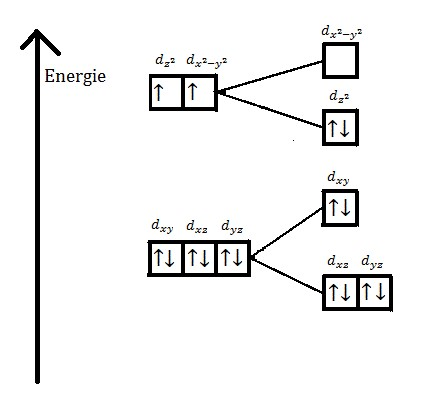
\includegraphics[scale=0.567]{Energieniveauskristallfeldtheorie.jpg}
\caption{Links ist die Aufspaltung der Orbitale im Oktaederfeld dargestellt, rechts die Aufspaltung durch Elongation der Bindungen in z-Richtung.}
\label{dsafigure:beispiel}
\end{dsafigure}

\subsection{Tetraeder}
Die Tetraeder Symmetrie ist äquivalent zur Würfelsymmetrie, da gilt: $\Delta_{t}=\frac{1}{2}\Delta_{w}$.
\cite{Koordinationsverbindung}
Bei einem Tetraeder geht die $z$-Achse durch zwei gegenüberliegende Kanten. Die größte Abstoßung findet auf Grund von elektrostatischer Wechselwirkung zwischen zwei Achsen statt. Aus diesem Grund werden in diesem Fall das $d_{xy}$, $d_{xz}$ und das $d_{yz}$-Orbital um $\frac{2}{5}\Delta$t angehoben, während das $d_{z^2}$ und das $d_{x^2 - y^2}$ Orbital um $\frac{3}{5} \Delta_t$ stabilisiert werden. In diesem Fall ist $\Delta _{t}$ allerdings größer als bei einem Oktaeder.

\section{Koordinationsverbindungen II - Ligandenfeldtheorie}
\authors{Lynn Meeder, Patricia Mühren}

Die Kristallfeldtheorie beschreibt Koordinationsverbindungen, wobei die Liganden klassisch betrachtet werden und das Zentralatom/-ion quantenmechanisch beschrieben wird. Ein genaueres Modell ist die Ligandenfeldtheorie, in der sowohl das Zentralatom/-ion als auch die Liganden sowie ihre Wechselwirkungen quantenmechanisch betrachtet werden.

\subsection{Ligandenfeldtheorie und 18-Elektronen-Regel}

Analog zur Oktettregel lässt sich die 18-Elektronen-Regel für Nebengruppenelemente formulieren. Wenn das System 18 Valenzelektronen hat, so ist die Komplexbildung stabil \cite{Huheey}.

Die Liganden sorgen auch in diesem Modell, genau wie bei der Kristallfeldtheorie, für eine Aufspaltung der Energieniveaus der $d$-Orbitale des Zentralatoms/-ions. Dabei bilden die $d_{z^2}$- und $d_{x^2-y^2}$-Orbitale des Zentralatoms/-ions mit zwei symmetrieadaptierten Linearkombinationen (SALCs) der Liganden zwei bindende und zwei antibindende Orbitale. Die bindenden Orbitale liegen auf einem energetisch niedrigeren Niveau und werden als $e_g$-Orbitale bezeichnet. Auf einem höheren Energieniveau liegen die antibindenden $e^*_g$-Orbitale. Die energetisch niedriger liegenden $d_{xy}$-, $d_{xz}$- und $d_{yz}$-Orbitale  werden als $t_{2g}$-Orbitale bezeichnet und sind nicht bindend.

Das unbesetzte $s$-Orbital des Zentralatoms/-ions bildet mit einem der SALCs der Liganden das komplett symmetrische $a_{1g}$-Orbital und das entsprechende antibindende $a^*_{1g}$-Orbital. Die drei unbesetzten $p$-Orbitale des Zentralatoms/-ions bilden mit drei SALCs der Liganden die bindenden, dreifach entarteten $t_{1u}$-Orbitale und ebenfalls die entsprechenden antibindenden $t^*_{1u}$-Orbitale.

Die Aufspaltungsenergie $\Delta_0$ beschreibt die Energiedifferenz zwischen den $e^*_g$- und $t_{2g}$-Orbitalen (siehe Abbildung \ref{Level}).

\begin{dsafigure}
	\centering
	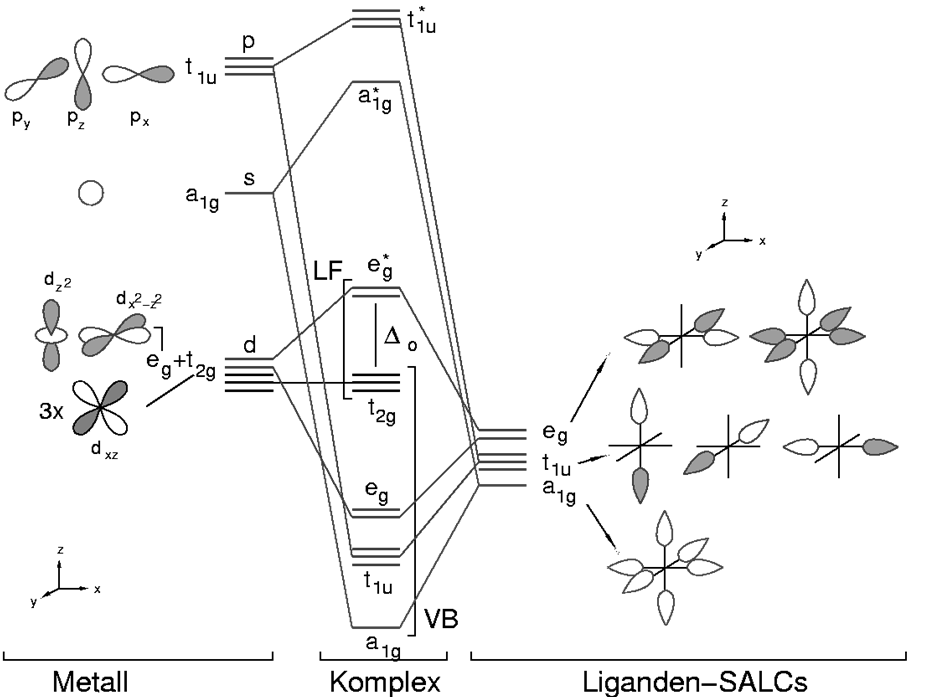
\includegraphics[width=\columnwidth]{EnergielevelKomplex.png}
	\caption{Die Molekülorbitale einer oktaedrischen Koordinationsverbindung \cite{Chemie_der_Metalle}}
	\label{Level}
\end{dsafigure}

Wie in Abbildung \ref{Level} sichtbar, gibt es sechs bindende und drei nicht bindende Orbitale. Die stärkste Bindung erhält man also, wenn diese neun Orbitale voll -- also mit 18 Elektronen -- besetzt sind. Damit lässt sich nun die 18-Elektronen-Regel begründen. 

Diese Regel gilt nun allerdings wie Abbildung \ref{Level}  nur für oktaedrische Komplexverbindungen. Bei anderen Koordinationsgeometrien unterscheidet sich das Molekülorbitalschema und dadurch kann eine andere Zahl an Valenzelektronen stabil sein.



\section{Fluoreszenz}
\authors{Ole Simmering, Ailin Sigel}

Fluoreszenz ist die Emission von Energie in Form von Licht kurz nach der Anregung eines Systems \cite{Atkins2001}. Dabei wird das gesamte System zuerst vertikal in einen höheren elektronischen Zustand angeregt (siehe Abbildung \ref{fig:Energiegraphen der elektronischen Zustände bei der Fluoreszenz}) und begibt sich dann zunächst strahlungslos in den Schwingungsgrundzustand des angeregten elektronischen Zustandes (siehe Abbildung \ref{fig:Energieniveaus der Fluoreszenz}). Nun fällt das System in den elektronischen Grundzustand zurück. Hierbei wird weniger Energie in Form von Licht frei, als vorher absorbiert wurde, um das System in den angeregten Zustand zu bringen.

\begin{dsafigure}
	\centering
	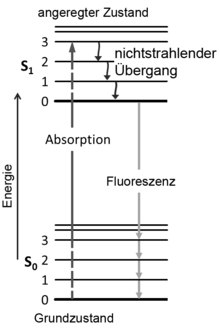
\includegraphics[width=4cm]{Fluoreszenz_Energieniveaus.png}
	\label{fig:Energieniveaus der Fluoreszenz}
	\caption{Energieniveauschema der Fluoreszenz \cite{wikiJablonskiDiagramm}.}
\end{dsafigure}

Es gilt für das Potential zweier gebundener Kerne: Bei sehr großer Nähe der Kerne läuft das Potential gen unendlich. Bei hinreichendem Abstand erreicht das Potential ein Minimum und nähert sich bei größerem Abstand einem Energiewert an (siehe Abbildung \ref{fig:Energiegraphen der elektronischen Zustände bei der Fluoreszenz}).

\begin{dsafigure}
	\centering
	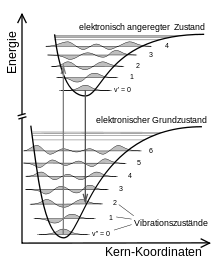
\includegraphics[width=5cm]{Fluoreszenz_Energie_Graph_elektronische_Zustaende.png}
	\label{fig:Energiegraphen der elektronischen Zustände bei der Fluoreszenz}
	\caption{Potentialkurven zweier elektronischer Zustände in Abhängigkeit des Kernabstandes in einem fluoreszierenden System \cite{wikiFranckCondonPrinzip}.}
\end{dsafigure}

Nach dem Franck-Condon-Prinzip gilt, dass der Übergang zwischen elektronischen Zuständen so verläuft, dass die Kernwellenfunktionen einen maximalen Überlapp haben. Zudem wird angenommen, dass die Anregung (und Bewegung der Elektronen) so schnell abläuft, dass die Kernbewegung ignoriert werden kann. Atomkerne sind rund 2000-mal schwerer als Elektronen und bewegen sich daher oft entsprechend langsamer. In Abbildung \ref{fig:Energiegraphen der elektronischen Zustände bei der Fluoreszenz} kann man sehen, dass die Pfeile als Darstellung für den Übergang vertikal verlaufen. Beschrieben wird dies durch die Franck-Condon-Näherung, die unter anderem besagt, dass die Wahrscheinlichkeit der Emission dort am höchsten ist, wo die Kernwellenfunkionen den größten Überlapp haben (siehe Abbildung \ref{fig:Energiegraphen der elektronischen Zustände bei der Fluoreszenz}).

%\section{Chemolumineszenz}

\section{Chemolumineszenz von Luminol -- Experiment}
\authors{Ailin Sigel, Jonas R. Stöckmann}

\subsubsection*{Chemikalien}

Destilliertes Wasser wird in diesem Versuch als Lösungsmittel verwendet.
\begin{enumerate}

\item Stammlösung L1
\begin{itemize}
\item 1 g Luminol ($C_8H_7N_3O_2$, 177,16$\frac{g}{mol}$)
\item 50 ml 10\%ige Natronlauge ($NaOH$, 39,997$\frac{g}{mol}$)
\item auf 500 ml aufgefüllt
\end{itemize}

\item Stammlösung L2
\begin{itemize}
\item 15 g Kaliumhexacyanoferrat(III) ($K_3[Fe(CN)_6]$, 329,26 $\frac{g}{mol})$)
\item auf 500 ml aufgefüllt 
\end{itemize}
\end{enumerate}

\subsubsection*{Durchführung} 

\begin{enumerate}

\item Grundlösung G1
\begin{itemize}
\item 30 ml L1 
\item auf 250 ml aufgefüllt
\end{itemize}

\item Grundlösung G2
\begin{itemize}
\item 30 ml L2 
\item 2 ml 30\%iges Wasserstoffperoxid ($H_2O_2$, 34,02$\frac{g}{mol}$)
\item auf 250 ml aufgefüllt 
\end{itemize}
\end{enumerate}

Mit den Stammlösungen L1 und L2 werden die Grundlösungen G1 und G2 nach der obigen Zusammensetzung hergestellt. Es entstehen somit je 250 ml von G1 und G2. 
In einem abgedunkelten Raum werden beide Grundlösungen gleichzeitig in ein Becherglas zusammengegeben. 

\subsubsection*{Beobachtungen}
Beim Zusammengeben von G1 und G2 und danach emittiert die entstandene Lösung blaues Licht. Die Lumineszenz nimmt mit der Zeit ab, es findet ein Farbwechsel von Neongrün zu Blau und anschließend zu dunkelblau statt. Zudem erscheint die Lösung nach Einschalten des Lichts klar. 

\subsubsection*{Hypothesen}
\begin{itemize}
\item Energie wird in Form von Licht freigesetzt
\item es findet eine Reaktion statt
\item Farbwechsel durch Sinken der Intensität
\item farbiger Anteil von G2 reagiert ab
\end{itemize}

Um die Hypothesen zu bestätigen oder zu widerlegen, werden acht Versuche durchgeführt, die sich unter anderem mit der Veränderung der Temperatur und der Konzentration der Edukte, sowie mit der Abnahme der Intensität mit der Zeit und der Rückreaktion beschäftigen.

Als Kamera wurde eine Canon70D verwendet mit einem ISO von $1000$, einer Blende von $4.0$ und einer Belichtungsdauer von $\frac{1}{20}$ s. Es wurden Bilder im Abstand von ca. 2 Sekunden gemacht. Das Becherglas und die Kamera hatten einen Abstand von ca. 46,5 cm.
%K_3 [Fe(CN)_6] 

\subsection{Konzentrationsveränderung von L1} 

Lynn Meeder, Selin Güler

\subsubsection{Versuchsbeschreibung}

Zunächst wird untersucht, wie sich eine Konzentrationsveränderung des Luminols und der Natronlauge (G1) auf den Reaktionsverlauf auswirkt. G2 bleibt während beider Varianten des Experimentes konstant. 

\subsubsection{Beobachtung}

Bei hoher Konzentration des Luminols und der Natronlauge ($G1^+$) ist eine sehr schnelle Reaktion zu beobachten. Auch ist direkt nach dem Zusammengeben von $G1^+$ mit der Lösung von G2 ist ein sehr starkes Leuchten zu sehen, das jedoch schnell an Intensität verliert. Die Intensität des emittierten Lichtes ist bereits nach 4 Sekunden so gering, dass die verwendete Kameraeinstellung aufgrund der schwachen Lumineszenz keine Bildaufnahme zulässt. Setzt man die Grundlösung aus der Stammlösung G1 mit halber Konzentration an, ergibt sich eine Grundlösung ($G1^-$), die bei der Reaktion mit G2 so wenig Licht emittiert, dass die Kamera bereits zu Beginn der Reaktion nicht auslöst.

\subsubsection{Auswertung}

Zusammenfassend kann gesagt werden, dass das Erhöhen der Konzentration von G1 die Reaktionsgeschwindigkeit ansteigen lässt und ein intensiveres Licht emittiert wird. Wenn die Konzentration von G1 herabgesetzt wird, tritt der gegenteilige Effekt ein.
\subsection{Konzentrationsänderung von Kaliumhexacyanoferrat(III)}
\authors{David Bürg, Patricia Mühren}

\subsubsection{Durchführung}

Um die Auswirkungen der Konzentration von $\mathrm{K}_3[\mathrm{Fe}(\mathrm{CN})_6]$ auf die Lumineszenz beschreiben zu können, wird die Grundlösung (G2) mit zwei verschiedenen Konzentrationen von $\mathrm{K}_3[\mathrm{Fe}(\mathrm{CN})_6]$ mit der gleichen Vorgehensweise in aufeinanderfolgenden Versuchen angereichert. Die erste Variation ist die G2-Lösung aus 15 ml L2 und 2 ml $\mathrm{H}_2\mathrm{O}_2$ ($\mathrm{G}2^-$), die andere eine G2-Lösung aus 60 mL L2 und 2 ml $\mathrm{H}_2\mathrm{O}_2$ ($\mathrm{G}2^+$). Zu den Grundlösungen wird dann demineralisiertes Wasser hinzugegeben, damit später wieder die 250-ml-Marke erreicht wird.
Dieser Versuch wird mit beiden Grundlösungen ($\mathrm{G}2^-$) und $\mathrm{G}2^+$), wie zuvor beschrieben, durchgeführt. Nach dem Zusammenschütten von G1 und G2 werden in konstanten Zeitintervallen Aufnahmen getätigt.
 
\subsubsection{Beobachtungen}

Bei der Zusammengabe von G1 und $\mathrm{G}2^-$ beobachtet man eine Emission von blauem beziehungsweise türkisem Licht.
Aus den Aufnahmen [Abb. \ref{dsafigure:beispiel1}] geht hervor, dass mit fortschreitender Zeit die Intensität des emittierten Lichtes abnimmt. Vergleicht man die vorher genannten Aufnahmen mit den Aufnahmen von $\mathrm{G}2^+$, so kann man feststellen, dass die Intensität des emittierten Lichtes bei $\mathrm{G}2^+$ höher ist als bei allen Aufnahmen von $\mathrm{G}2^-$. Diese Beobachtung wird auch mit technisch ermittelten  Werten durch ImageJ \cite{ImageJ}, siehe Tabelle \ref{dsatable:beispiel0}, belegt. Bei der Ermittlung der Intensität wird über den Grauwert entlang einer rechteckigen Fläche integriert.  

\begin{dsatable}
 \caption{Intensitätswerte des emittierten Lichtes für die einzelnen Aufnahmen von unterschiedlichen          Bechergläsern, einmal mit $\mathrm{G}2^+$ und das andere Mal mit $\mathrm{G}2^-$. Dabei entstehen beim Festhalten der Intensität der Lumineszenz mit der Grundlösung von 15 ml $\mathrm{K}_3[\mathrm{Fe}(\mathrm{CN})_6]$ vier Aufnahmen, mit der Grundlösung von 60 ml $\mathrm{K}_3[\mathrm{Fe}(\mathrm{CN})_6]$ eine Aufnahme.}
 \centering
 \begin{tabular}{lcr}
  \toprule
   Zeit            & Intensitätswert\\
  \midrule
   2 s			   & 58.013\\
   4 s		       & 47.016\\
   6 s		       & 36.886\\
   8 s		       & 28.978\\
  \midrule
   2 s		       & 72.5588\\
  \bottomrule
 \end{tabular}
 \label{dsatable:beispiel0}
\end{dsatable}

\begin{dsafigure}
 \centering
 \includegraphics[scale=0.05]{G2minusSeriemitSekunden.jpg}
 \caption{G1 und $\mathrm{G}2^-$ --> Aufnahme nach zwei, vier, sechs und acht Sekunden}
 \label{dsafigure:beispiel1}
\end{dsafigure} 

\subsection{Konzentrationsänderung des Wasserstoffperoxids $H_{2}O_{2}$}
Isabelle Schulte-Herbrüggen, Kristina Heuser
Der zu Beginn erläuterten Versuch wurde mit einer verdoppelten Menge an Wasserstoffperoxid durchgeführt.

Nach Zusammenführen der beiden Lösungen war eine Emission von blauem Licht zu erkennen, dessen Leuchten mit der Zeit abgenommen hat. Die Intensität der Farbe wurde nicht beeinflusst, jedoch war diese schon nach einer Aufnahme zu gering, um weitere Fotos zu machen. Dies weist auf eine höhere Reaktionsgeschwindigkeit als beom Ausgangsversuch hin. 
\subsection{Temperaturänderung während der Reaktion}
\authors{Ailin Sigel, Jonas R. Stöckmann}

Reaktionen nehmen häufig Energie in Form von Wärme auf oder geben Energie in Form von Wärme ab. Um die Hypothese der Reaktion zu untermauern, wird zunächst die Temperatur während der Reaktion gemessen. Diese beträgt 25 $^\circ$C. Es fand keine Temperaturänderung statt. Nach sechs Minuten war keine Lumineszenz mehr zu beobachten. 



\subsection{Temperaturabhängigkeit}
\authors{Johannes Wörsdörfer}
\subsubsection{Durchführung}
Für diesen Versuch werden die Gemische G1 und G2 auf 10$^\circ$ C abgekühlt. Anschließend werden sie, wie im allgemeinen Teil beschrieben, gemischt. Als Referenzwert werden beim zweiten Versuch die Gemische nicht abgekühlt, um eine Starttemperatur von ca. 20 $^\circ$C (Raumtemperatur) zu erreichen.

\subsubsection{Beobachtung}
Bei einer geringen Starttemperatur von ca. 10 $^\circ$C lässt sich eine schwächere Intensität des Lichtes als bei einer Starttemperatur von 20 $^\circ$C messen (siehe Tabelle \ref{table:Temperatur}). Allerdings bleibt die Lumineszenz in der kalten Lösung länger erhalten als in der Lösung bei Raumtemperatur. Genaue Werte dessen wurden jedoch nicht gemessen. Somit handelt es sich bei der Dauer der Lumineszenz um eine weitgehend subjektive Beobachtung.

\begin{dsatable}
 \caption{Messung der Intensität der Lumineszenz der Gemische bei 10 $^\circ$C und bei 20 $^\circ$C.}
 \centering
 \begin{tabular}{crr} 
  \toprule
  Zeit      &  10 $^\circ$C  &  20 $^\circ$C \\
  \midrule
   2s		& 10,09 	& 15,54 \\
   4s		& 8,55		& 9,76	\\
   6s		&  			& 6,76	\\
   8s		& 			& 4,82	\\
  \bottomrule
 \end{tabular}
 \label{table:Temperatur}
\end{dsatable}

\subsubsection{Auswertung}
Durch das Absenken der Temperatur wird die Bewegung der Teilchen verlangsamt. Somit treffen die Edukte seltener aufeinander. Dies verringert die Reaktionsgeschwindigkeit, sodass das Gemisch schwächer Licht emittiert. Außerdem dauert es länger, bis sich ein Reaktionsgleichgewicht einstellt, sodass die Lumineszenz länger erhalten bleibt. 

\subsection{Zeitabhängigkeit der Lumineszenz} 
\authors{Gala Gottschalg, Sophia Ivaschuk}

Im zuvor beschriebenen Versuch wurden alle zwei Sekunden Intervall-Aufnahmen aufgenommen. Dabei wurden die vier Photographien untereinander verglichen und die Intensität der Lumineszenz ermittelt. Die Ergebnisse sind in Tabelle \ref{dsatable:Zeitabhaengigkeit} angegeben.

\begin{dsatable}
 \caption{Zeitabhängigkeit der Lumineszenz.}
 \centering
 \begin{tabular}{lr} % zwei Spalten
  \toprule
  Zeit &  Intensitätswert\\
  \midrule
  2 Sekunden      & 84.8746\\
  4 Sekunden      & 52.4111\\
  6 Sekunden      & 35.0930\\
  8 Sekunden      & 24.4441\\
  \bottomrule
 \end{tabular}
 \label{dsatable:Zeitabhaengigkeit}
\end{dsatable}


Die rechte Spalte der Tabelle zeigt die relative Intensität der Lumineszenz im Versuchsverlauf. Wie man den Tabellenwerten entnehmen kann, ist der Verlauf der Intensitätskurve nicht linear. Stattdessen verringert sich die Intensität zunächst stärker, wobei anschließend die Abnahme von Bild zu Bild geringer wird, bis sie sich final einem Wert von null annähert und der Vorgang der Lumineszenz abgeschlossen ist.
Dies wird besonders in Abbildung \ref{fig:Intensitaet} deutlich, in der die Werte der Intensität dargestellt sind.

\begin{dsafigure}
 \centering
 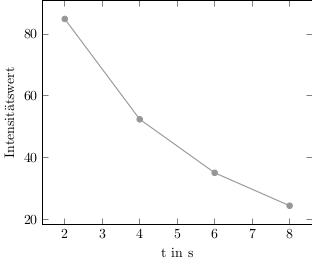
\includegraphics[width=\columnwidth]{Graph_Intensitaet}
 \caption{Verlauf der Intensitätswerte.}
 \label{fig:Intensitaet}
\end{dsafigure}



\subsection{Farbigkeit}

Ole Simmering, Lena Prahe 

Im siebten Teilexperiment wurden die Photographien des sechsten Versuches genutzt und auf die Farbe der Reaktion untersucht. Im Folgenden sind die RGB-Werte, also die Rot-, Grün- und Blauanteile und die entsprechenden HSL-Werte, also der Farbwert, der Sättigungswert und der Helligkeitswert dargestellt (siehe Tab. \ref{RGB-Werte_Tabelle} und Abb. \ref{Diagramm_H_ueber_t}). Der Farbwert wird als Farbwinkel H auf dem Farbkreis (etwa 0$^\circ$ für Rot, 120$^\circ$ für Grün, 240$^\circ$ für Blau) angegeben. So konnten wir mit dem Farbwert der Reaktion vergleichen, wie sich die Farbe über die Zeit verändert, ohne den Intensitätsverlauf zu berücksichtigen.

\begin{dsatable}
 \centering
 \caption{RGB-Werte und HSL-Werte der Bilder von der Reaktion.}
 \begin{tabular}{lcc} % vier Spalten
  \toprule
   Zeit  & RGB & HSL\\
  \midrule
   nach 2 s  & 2, 125, 124 &   180, 96.9\%, 24.9\%    \\
   nach 4 s  & 2, 83, 86   &   182, 95.5\%, 17.3\%    \\
   nach 6 s  & 1, 48, 58   &   191, 96.6\%, 11.6\%    \\
   nach 8 s  & 1, 31, 42   &   196, 95.3\%, 8.4\%     \\ 
  \bottomrule
 \end{tabular}
 \label{RGB-Werte_Tabelle}
 
\end{dsatable}

\begin{dsafigure}
	\centering
	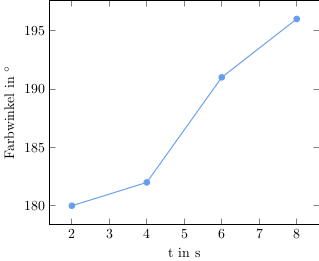
\includegraphics[width=7cm]{figure0.png}
	\label{Diagramm_H_ueber_t}
	\caption{Abhängigkeit des Farbwinkels im Farbkreis von der Zeit.}
\end{dsafigure}

Diese Werte ergaben sich aus einer Analyse der RGB-Werte eines fixen Bildpunktes in der Bilderserie der Reaktion mithilfe des Grafikeditors GIMP \cite{GIMP}. Die RGB-Werte wurden mittels des Online-Rechners RapidTables \cite{RapidTables} zu HSL umgerechnet. Es ist erkennbar, dass sich der Farbwinkel fast nicht ändert (siehe Abb. \ref{Diagramm_H_ueber_t}). Es ist vermutlich nur ein Stoff für die Farbgebung verantwortlich, da die Farbe des Lichtes fast konstant bleibt.

\subsection{Durchf\"uhrung}
Joes Biburger, Ali Serour

Nach dem Erl\"oschen der Lumineszenz wurde weitere Natronlauge hinzugegeben.
\subsubsection{Beobachtung und Deutung}
Nach der Zugabe von Natronlauge leuchtete die L\"osung kurzzeitig wieder schwach.
Daraus kann man schließen, dass durch die Zugabe von Natronlauge das System aus dem Gleichgewicht gebracht wurde, wodurch eine erneute Reaktion folgte.


\section{Chemolumineszenz}

%\authors{Jonas R. Stöckmann, Atousa Seyedian}
Bei der Chemolumineszenz handelt es sich um einen Prozess, der zur Lumineszenz führt. Hier sorgt ein Übergang in den elektronischen Grundzustand für die Emission von Licht. Im Gegensatz zu der Fluoreszenz oder Phosphoreszenz wird die Energie nicht durch externen Lichteinfall einer Lichtquelle aufgebracht, sondern durch eine chemische Reaktion.
Bei der Reaktion der Edukte entsteht das Produkt im angeregten Zustand. Zum Ende der Chemolumineszenz-Reaktion fällt das Produkt in den energetischen Grundzustand. 

\subsection{Das Licht der Chemolumineszenz}

Die Dauer des Leuchtens bei einer Chemolumineszenz ist vergleichbar mit der von Fluoreszenz. 
Die emittierten Lichtwellen befinden sich meist im sichtbaren Bereich des Spektrums und weisen Wellenlängen zwischen 400 und 700 nm auf. Aber auch in den Wellenlängenbereichen der Farben Ultraviolett und Infrarot kann nicht-sichtbares Licht emittiert werden. \cite{Doerfler}

\subsection{Energie der Chemolumineszenz}

Bei einer Chemolumineszenz wird hauptsächlich chemische Energie in Form von Licht und nicht nur (wie oftmals bei chemischen Reaktionen) in Form von thermischer Schwingungsenergie emittiert. Dabei wird vorausgesetzt, dass diese Energiefreisetzung auf einmal, das heißt nicht zwangsweise in mehreren Stufen erfolgt. Chandross und Sonntags Postulat von 1964 zum Thema Chemolumineszenz \cite{Chandross} besagt, dass die Reaktionsenthalpie (Energieumsetzung) in einem einzigen Reaktionsschritt, in geringer Zeit und in möglichst kleinem Volumen freigesetzt werden sollte.
Dennoch ist es möglich, dass ein Teil der Energie auch durch Schwingung abgegeben wird. 

\subsection{Ablauf der Reaktion}

Eines der bekanntesten Beispiele für Chemolumineszenz-Reaktionen ist die durch Kaliumhexacyanoferrat(III) katalysierte Oxidation von Luminol mit alkalischem Wasserstoffperoxid. 

\begin{dsafigure}
 \centering
 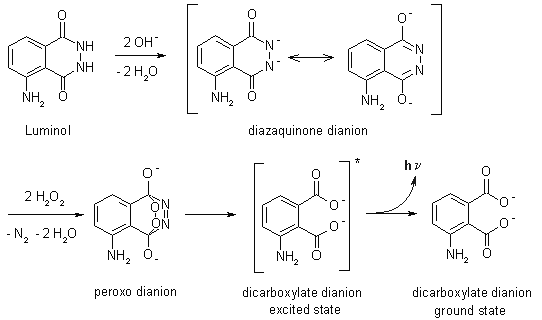
\includegraphics[width=8cm]{Chemolumineszenz_Reaktion_Luminol.png}
 \caption{Chemoluminszenz-Reaktion von Luminol. \cite{Cartus}}
 \label{dsafigure:Chemolumineszenz}
\end{dsafigure}

Das Luminol reagiert in alkalischem Milieu durch Angriff von Hydroxid-Anionen zum Dianion. Das Luminol agiert dabei als Broensted-Säure und reagiert mit den $ OH^{-} $-Ionen unter Abspaltung von $ H^{+} $-Ionen. Das so entstandene Dianion ist mesomeriestabilisiert. 
Bei der folgenden Oxidationsreaktion des Dianions mit Wasserstoffperoxid wird Stickstoff freigesetzt. Es entsteht ein angeregtes Zwischenprodukt, das 3-Amino-Phtalsäure-dianion. Dieses instabile Intermediat geht zuletzt unter Lichtemission in den energetischen Grundzustand über.  

\section{Phosphoreszenz}
\authors{Selin Güler, Joes Biburger}

Mit Phosphoreszenz wird die Emission von Licht bezeichnet, die auf einen Übergang von einem angeregten Triplett- in einen Singulett-Grundzustand zurückzuführen ist. 

Der Phosphoreszenzvorgang beginnt mit der Absorption eines Photons mit spezifischer Wellenlänge durch ein Molekül. Letzteres wird vom Grundzustand in einen angeregten Singulettzustand $(S_1)$, in dem alle Elektronen mit entgegengesetztem Spin gepaart sind, angeregt. Nun erfolgt der als Intersystem Crossing bezeichnete Übergang in einen angeregten Triplettzustand $(T_1)$. In diesem gibt es zwei ungepaarte Elektronen mit gleichem Spin. Der angeregte Triplettzustand $(T_1)$ ist energieärmer und somit stabiler als der angeregte Singulettzustand $(S_1)$. Aufgrund der Tatsache, dass die für den Übergang in den Grundzustand $(S_0)$ notwendige Spinumkehr spinverboten und somit unwahrscheinlich ist, können mehrere Stunden vergehen, bevor das Molekül in den Grundzustand zurückfällt. Bei einem solchen Übergang wird Energie in Form von Licht abgegeben. Das emittierte Licht ist immer langwelliger als das bei der Anregung aufgenommene. Das rührt daher, dass bei der Phosphoreszenz, ähnlich wie bei der Fluoreszenz, verschiedene Schwingungszustände innerhalb des Grund- $(S_0)$ sowie angeregten Triplettzustandes $(T_1)$ existieren. Das Molekül gibt beim Übergehen in den energieärmsten Schwingungszustand Energie strahlungsfrei an weitere Translations-, Rotations-, Schwingungsmoden ab, weshalb nur ein Teil der Energie des absorbierten Lichtes in Form von Licht wieder emittiert wird. 
\cite{Phosphoreszenz1}, \cite{Phosphoreszenz2}, \cite{Phosphoreszenz3}



\section*{Literaturverzeichnis}
\bibliographystyle{jcpsty_deutsch}
%\bibliographystyle{unsrtdin}
\bibliography{lit2}

\end{document}
